\label{3.5 C7S Answer Key}
\subsection{Answer Key}
\tiny
\renewcommand{\insertclass}{- Class 7}
\renewcommand{\insertsubject}{ - Science}

\begin{frame}[shrink=0.1,label=QPC7QC7S01 - DT - Q7]{Q6 [1. Nutrition in Plants]}
\vspace{-0.2cm}
\mcqimgleftFourOne{
  questionnumber={6}, 
  questionTag={C7S01 – DT – Q7},
  questiontext={The given plant comes under the category of \rule{80pt}{0.1pt}.},
  imgtabletikz = { {\adjustbox{scale=\scalefactor}{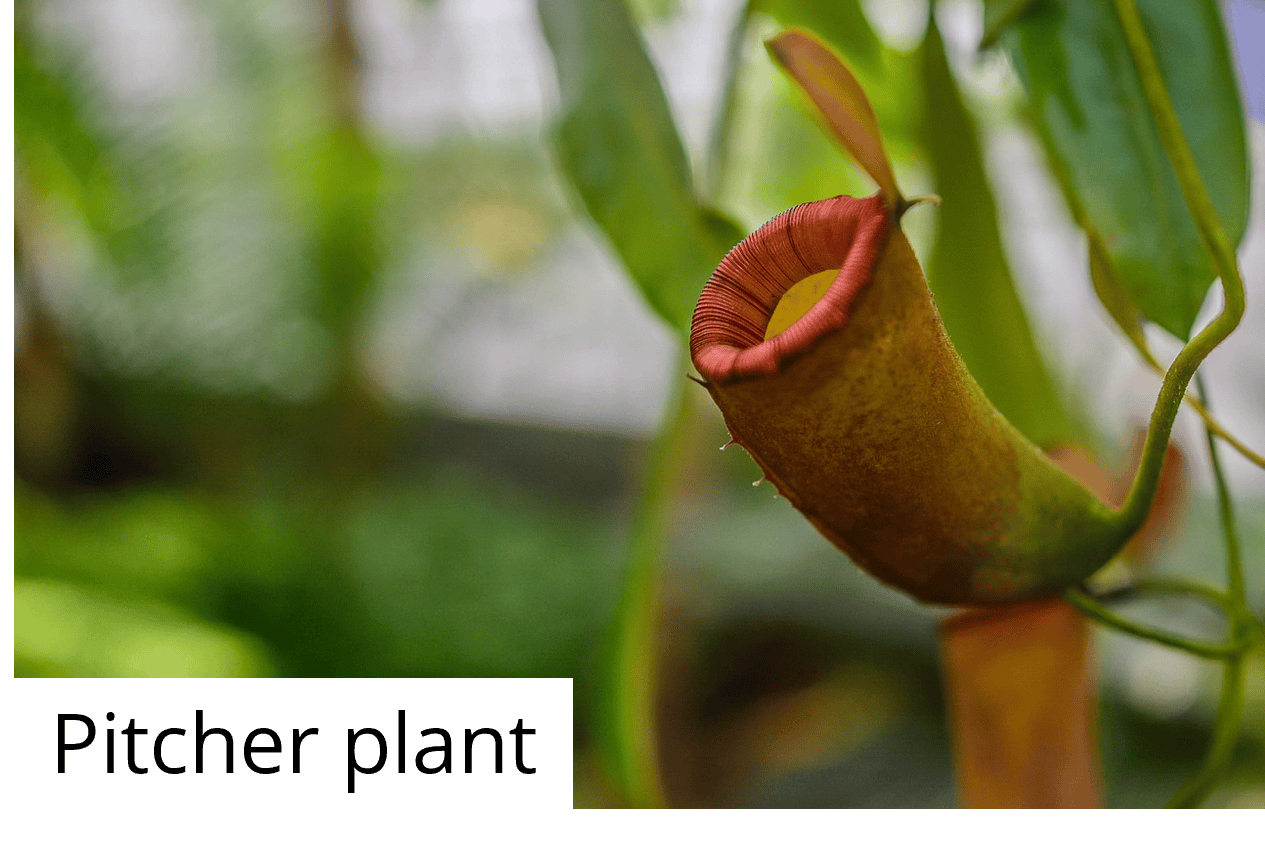
\includegraphics[width=3.75cm,height=2.7cm]{C7S01 – DT – Q7.png}}}  },
  optionA={Parasitic plants},
  optionB={Insectivorous plants},
  optionC={Saprotrophs},
  optionD={Symbiotic},
  correctoption={B},
  leftmini={0.5},
  rightmini={0.4},
}

\begin{minipage}{\linewidth}
\hspace{1cm}
\centering
\tiny
\renewcommand{\arraystretch}{1.25}
\begin{tabular}{|M{1.2cm}|M{0.8cm}|M{0.8cm}|M{0.8cm}|M{0.8cm}|M{0.8cm}|}
\hline
Option & A (\ding{55}) & \cellcolor{cellgreen} B (\ding{51}) & C (\ding{55}) & D (\ding{55}) & E \\ 
\hline
7 A & \highno{38\%} & \highno{63\%} & \highno{0\%} & \highno{0\%} & \highno{0\%} \\ 
 \hline 
7 B & \highno{43\%} & \highno{43\%} & \highno{7\%} & \highno{7\%} & \highno{0\%} \\ \hline
\end{tabular}
\end{minipage}

\end{frame}
% \input{4. PPT/6. My Answer/Science/C7/117_C7S - Q6}


\begin{frame}[shrink=0.1,label=QPC7QC7S01 - DT - Q11]{Q50 [1. Nutrition in Plants]}
\vspace{-0.2cm}

\matextbottomTwoTwo{
myanswerquestion={Fill in the blanks based on autotroph and heterotroph},
myanswercontent={\begin{enumerate}
    \item Organisms that can make their food using sunlight, water, and carbon dioxide are called \rule{100pt}{0.5pt}.
    \item Organisms that cannot make their food and rely on other organisms for energy are called \rule{100pt}{0.5pt}.
\end{enumerate}
},
questionnumber={50}, 
  questionTag={C7S01 - DT - Q11}, 
  questiontext={Identify the autotroph and heterotroph in the given picture.\\ \hspace{2cm}
\begin{tikzpicture}[x=0.75pt,y=0.75pt,yscale=-1,xscale=1]
\tikzset{every picture/.style={line width=0.75pt,scale=\scalefactor}}
\draw (327.33,67.83) node  {\adjustbox{scale=\scalefactor}{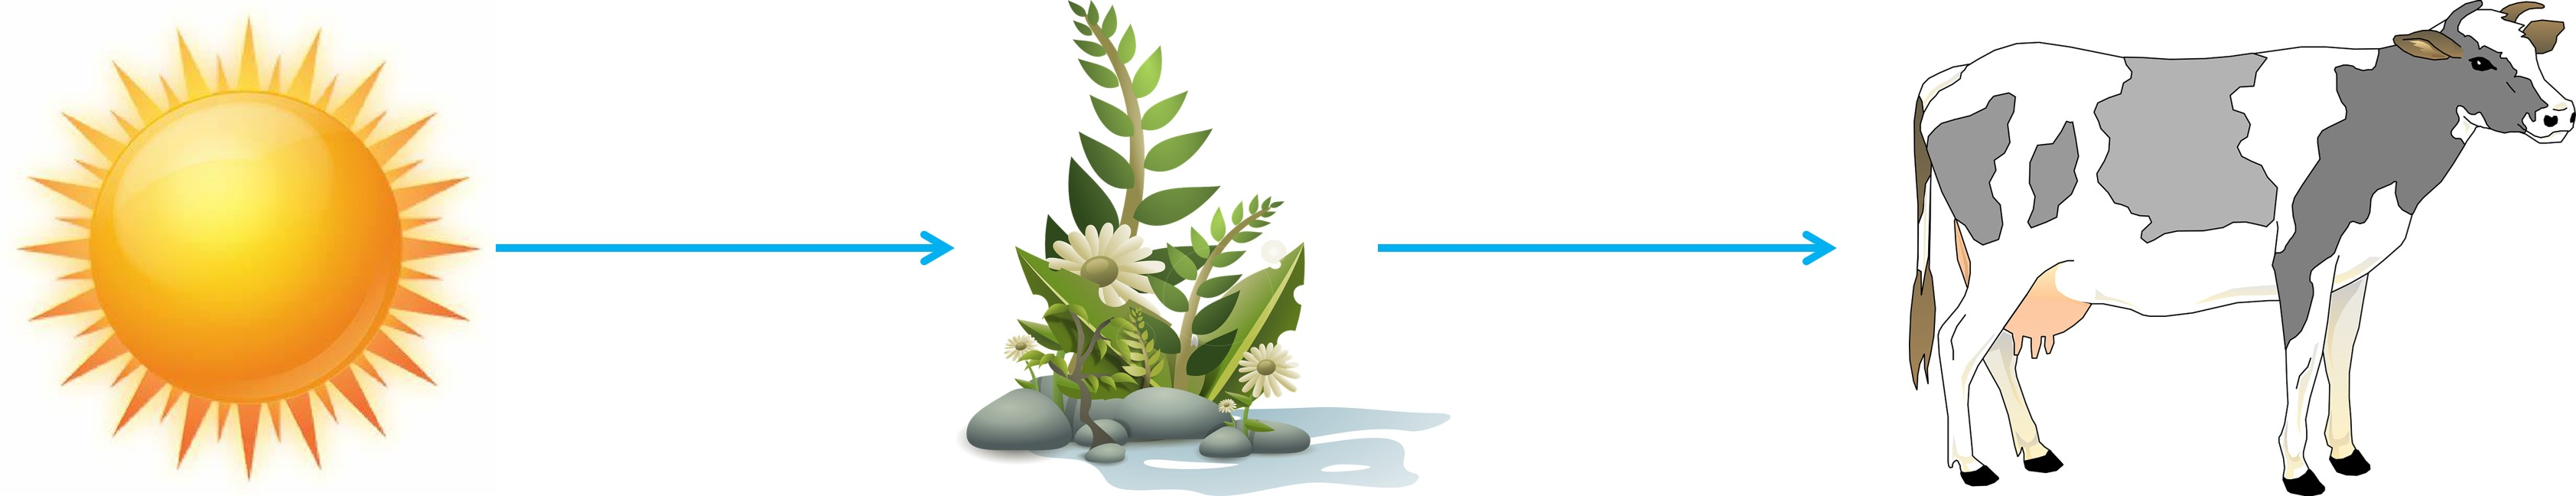
\includegraphics[width=336pt,height=55.75pt]{C7S01 – DT – Q2 .jpg}}};
\draw (160.75,100) node [anchor=north west][inner sep=0.75pt]   [align=left] {Sun};
\draw (300.25,100) node [anchor=north west][inner sep=0.75pt]   [align=left] {Plant};
\draw (460.25,100) node [anchor=north west][inner sep=0.75pt]   [align=left] {Cow};
\end{tikzpicture}
},
  optionA={Plant – Autotroph, Cow - Heterotroph},
  optionB={Plant – Heterotroph, Cow - Autotroph},
  optionC={Sun – Autotroph, Cow – Heterotroph },
  optionD={Both plant and sun are heterotrophs},
  correctoption={A},
}


\begin{minipage}{\linewidth}
\hspace{1cm}
\centering
\tiny
\renewcommand{\arraystretch}{1.25}
\begin{tabular}{|M{1.2cm}|M{0.8cm}|M{0.8cm}|M{0.8cm}|M{0.8cm}|M{0.8cm}|}
\hline
Option & \cellcolor{cellgreen} A (\ding{51}) & B (\ding{55}) & C (\ding{55}) & D (\ding{55}) & E \\ 
\hline
7 A & \highno{75\%} & \highno{13\%} & \highno{6\%} & \highno{6\%} & \highno{0\%} \\ 
 \hline 
7 B & \highgreen{86\%} & \highno{7\%} & \highno{0\%} & \highno{7\%} & \highno{0\%} \\ \hline
\end{tabular}
\end{minipage}

\end{frame}
\begin{frame}{Q50 - My Answer Responses}
    \vspace{-0.6cm}
    \begin{multicols}{2}

    % Image: Q50_D117185_Science.png - Scaled height: 2.29mm
    \begin{minipage}{\linewidth}
    \RaggedRight\textbf{\tiny \highred{Sujay Kumar N [C]}} \\ 
    \vspace{4.00pt}\fcolorbox{blue}{white}{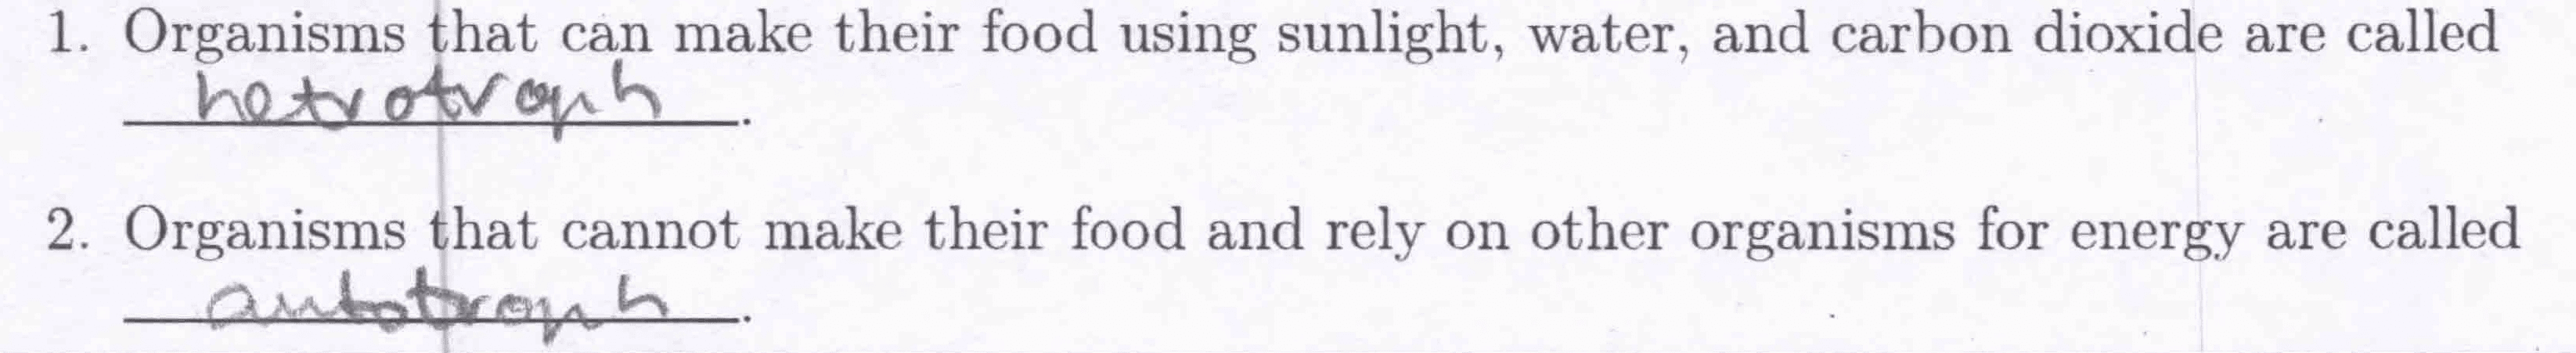
\includegraphics[width=6cm]{Q50_D117185_Science.png}}
    \end{minipage}
    \vspace{10pt}

    % Image: Q50_D117186_Science.png - Scaled height: 2.27mm
    \begin{minipage}{\linewidth}
    \RaggedRight\textbf{\tiny \highgreen{Yashwanth M [A]}} \\ 
    \vspace{4.00pt}\fcolorbox{blue}{white}{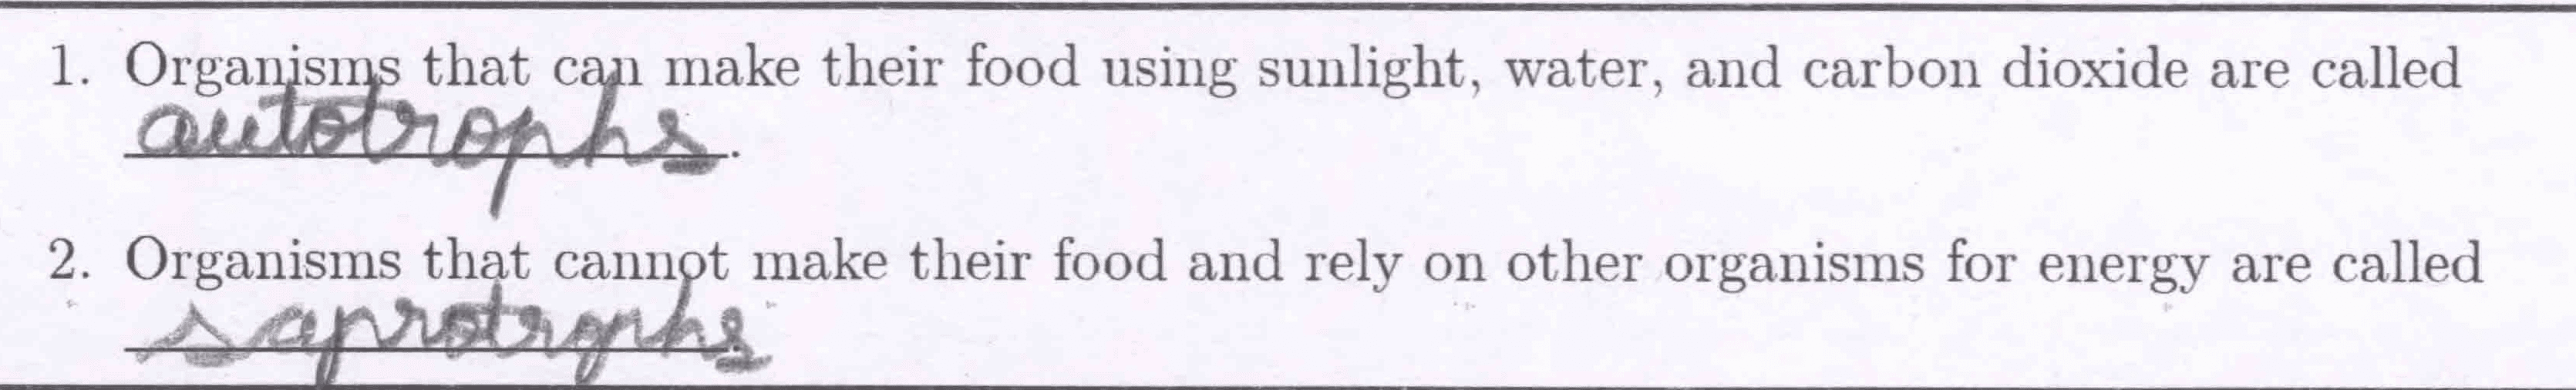
\includegraphics[width=6cm]{Q50_D117186_Science.png}}
    \end{minipage}
    \vspace{10pt}

    % Image: Q50_D117188_Science.png - Scaled height: 2.44mm
    \begin{minipage}{\linewidth}
    \RaggedRight\textbf{\tiny \highgreen{Anjali Mishra [A]}} \\ 
    \vspace{4.00pt}\fcolorbox{blue}{white}{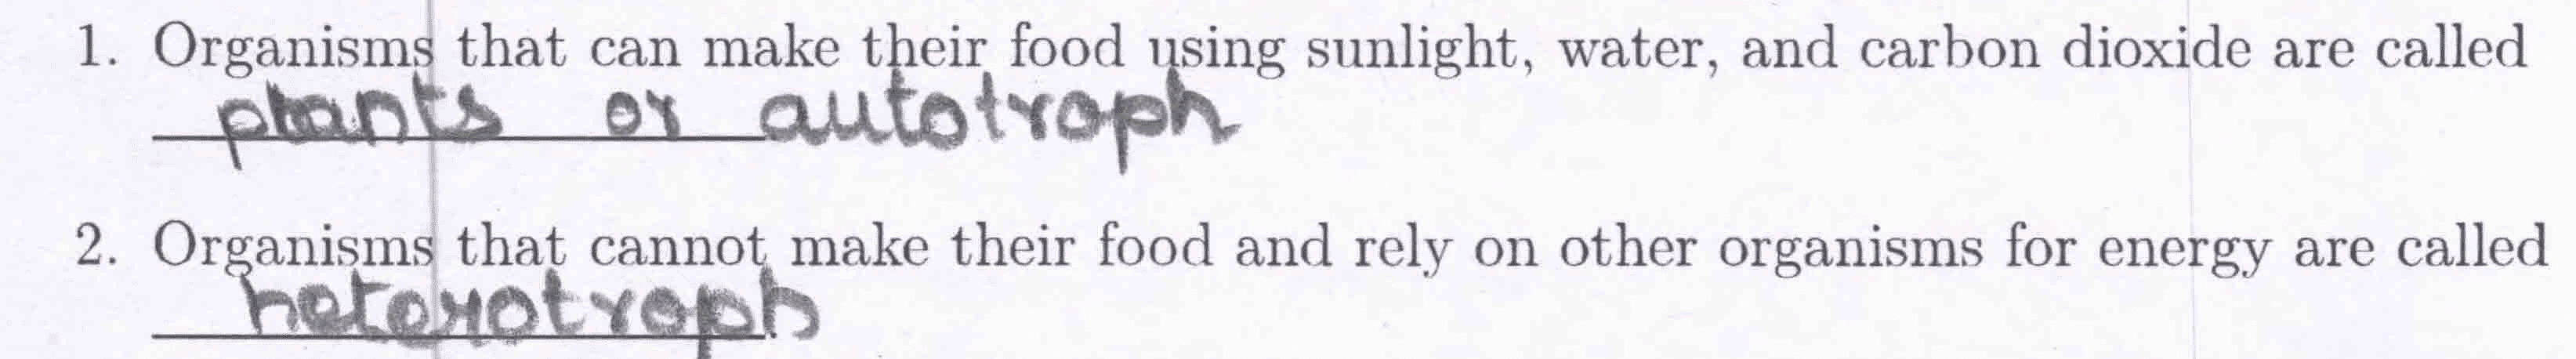
\includegraphics[width=6cm]{Q50_D117188_Science.png}}
    \end{minipage}
    \vspace{10pt}

    % Image: Q50_D117190_Science.png - Scaled height: 2.36mm
    \begin{minipage}{\linewidth}
    \RaggedRight\textbf{\tiny \highgreen{Mithra J R [A]}} \\ 
    \vspace{4.00pt}\fcolorbox{blue}{white}{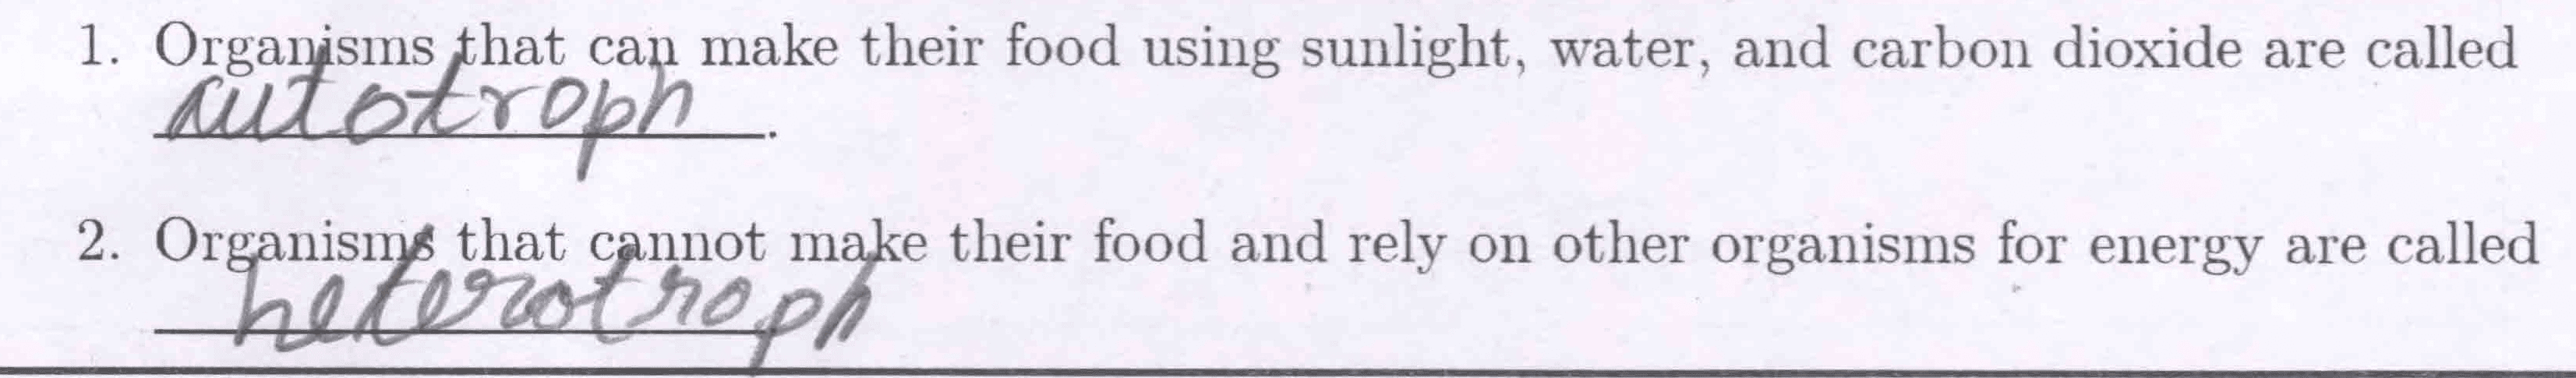
\includegraphics[width=6cm]{Q50_D117190_Science.png}}
    \end{minipage}
    \vspace{10pt}

    % Image: Q50_D117192_Science.png - Scaled height: 2.35mm
    \begin{minipage}{\linewidth}
    \RaggedRight\textbf{\tiny \highgreen{Shri Yashini P [A]}} \\ 
    \vspace{4.00pt}\fcolorbox{blue}{white}{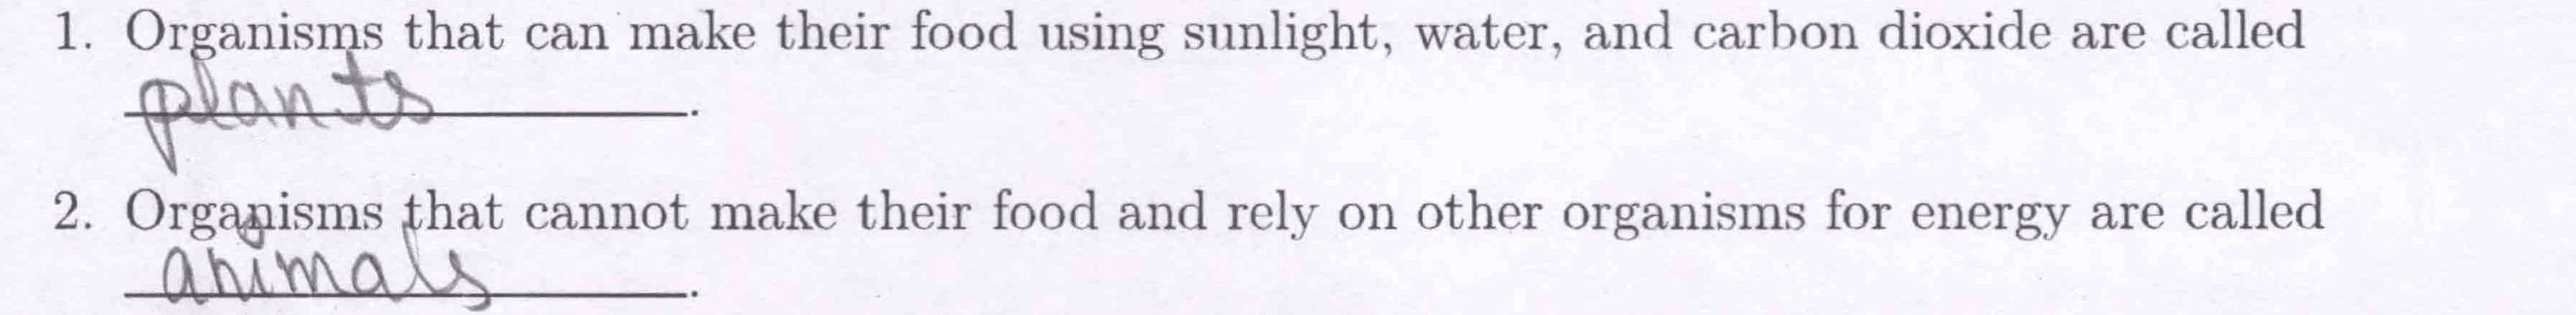
\includegraphics[width=6cm]{Q50_D117192_Science.png}}
    \end{minipage}
    \vspace{10pt}

   % Image: Q50_D117212_Science.png - Scaled height: 2.35mm
    \begin{minipage}{\linewidth}
    \RaggedRight\textbf{\tiny \highgreen{Tanvisha V [A]}} \\ 
    \vspace{4.00pt}\fcolorbox{blue}{white}{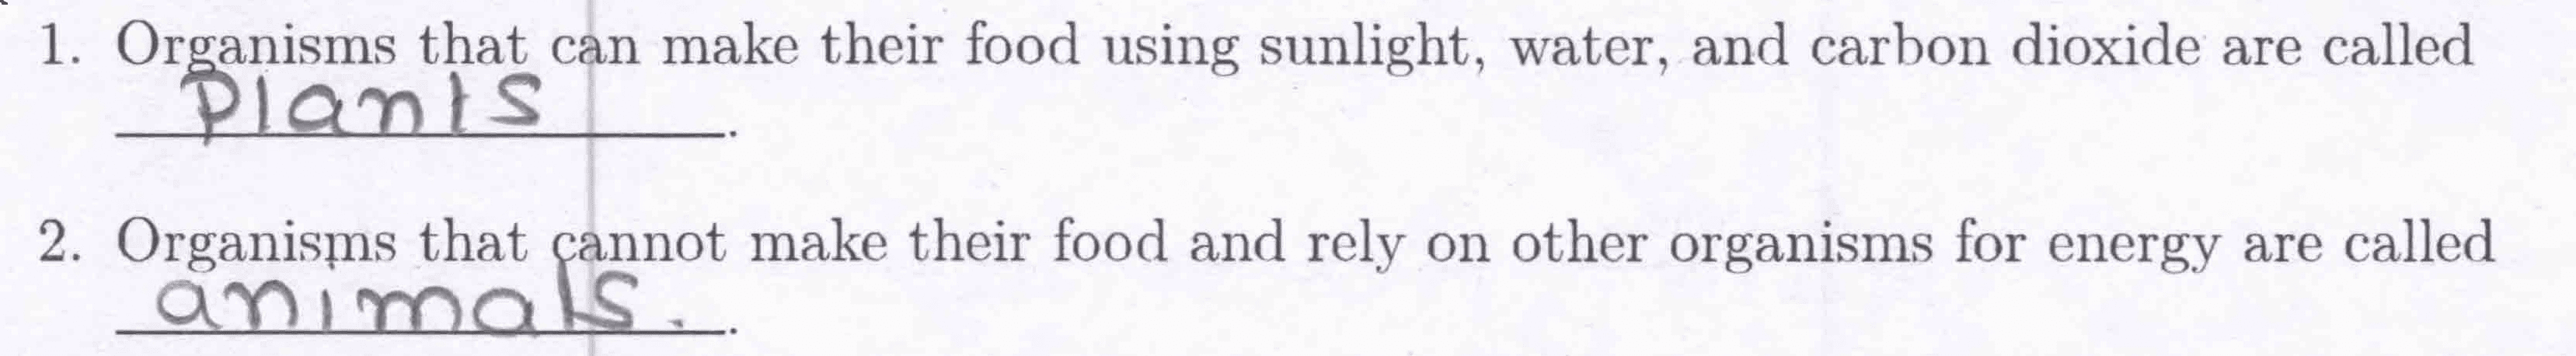
\includegraphics[width=6cm]{Q50_D117212_Science.png}}
    \end{minipage}
    \vspace{10pt}

    \end{multicols}
\end{frame}

\begin{frame}{Q50 - My Answer Responses}
    \vspace{-0.6cm}
    \begin{multicols}{2}

  % Image: Q50_D117194_Science.png - Scaled height: 2.41mm
    \begin{minipage}{\linewidth}
    \RaggedRight\textbf{\tiny \highgreen{Tharsika S [A]}} \\ 
    \vspace{4.00pt}\fcolorbox{blue}{white}{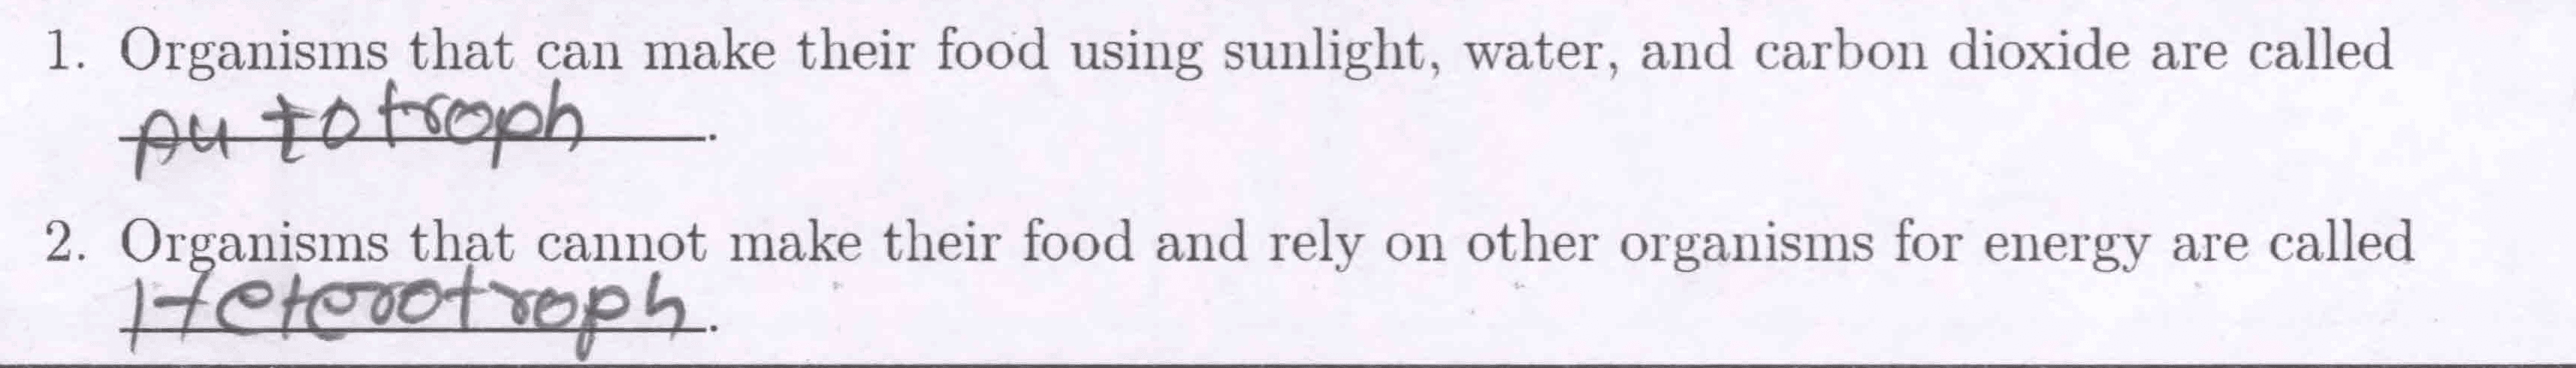
\includegraphics[width=6cm]{Q50_D117194_Science.png}}
    \end{minipage}
    \vspace{10pt}

    % Image: Q50_D117197_Science.png - Scaled height: 2.49mm
    \begin{minipage}{\linewidth}
    \RaggedRight\textbf{\tiny \highred{Dharshan K [B]}} \\ 
    \vspace{4.00pt}\fcolorbox{blue}{white}{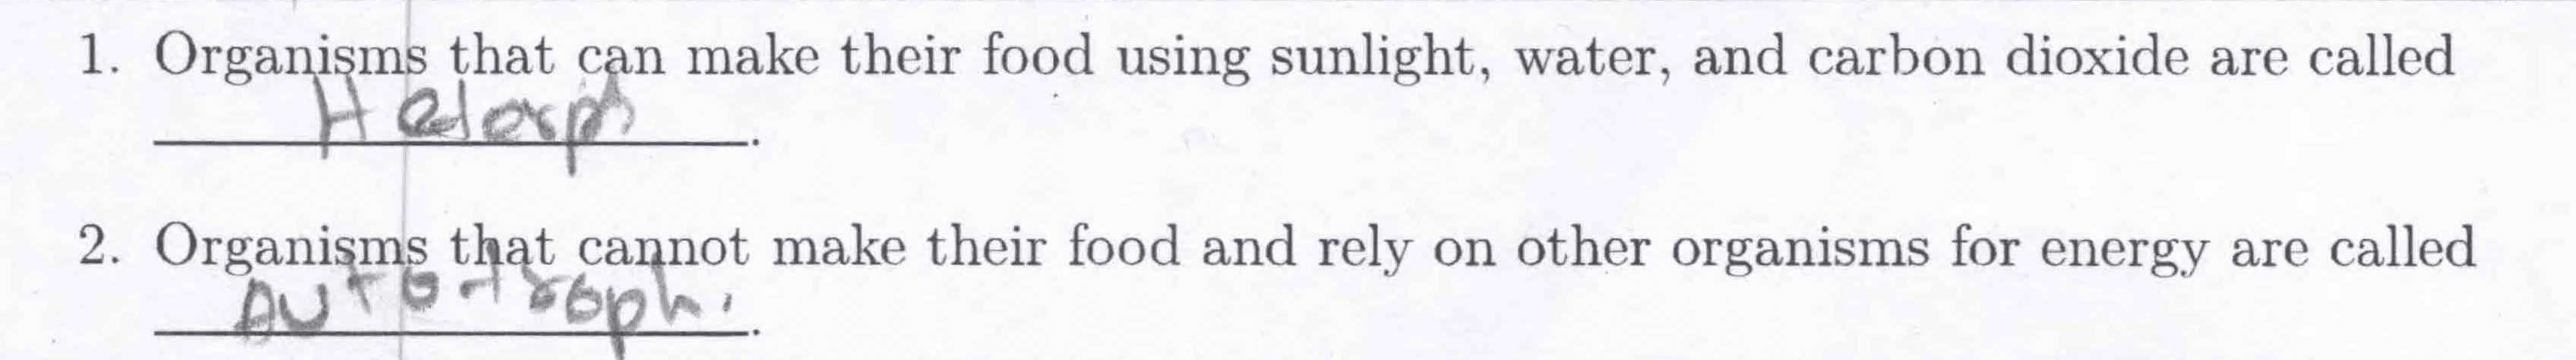
\includegraphics[width=6cm]{Q50_D117197_Science.png}}
    \end{minipage}
    \vspace{10pt}

    % Image: Q50_D117198_Science.png - Scaled height: 2.23mm
    \begin{minipage}{\linewidth}
    \RaggedRight\textbf{\tiny \highgreen{Eniyan E [A]}} \\ 
    \vspace{4.00pt}\fcolorbox{blue}{white}{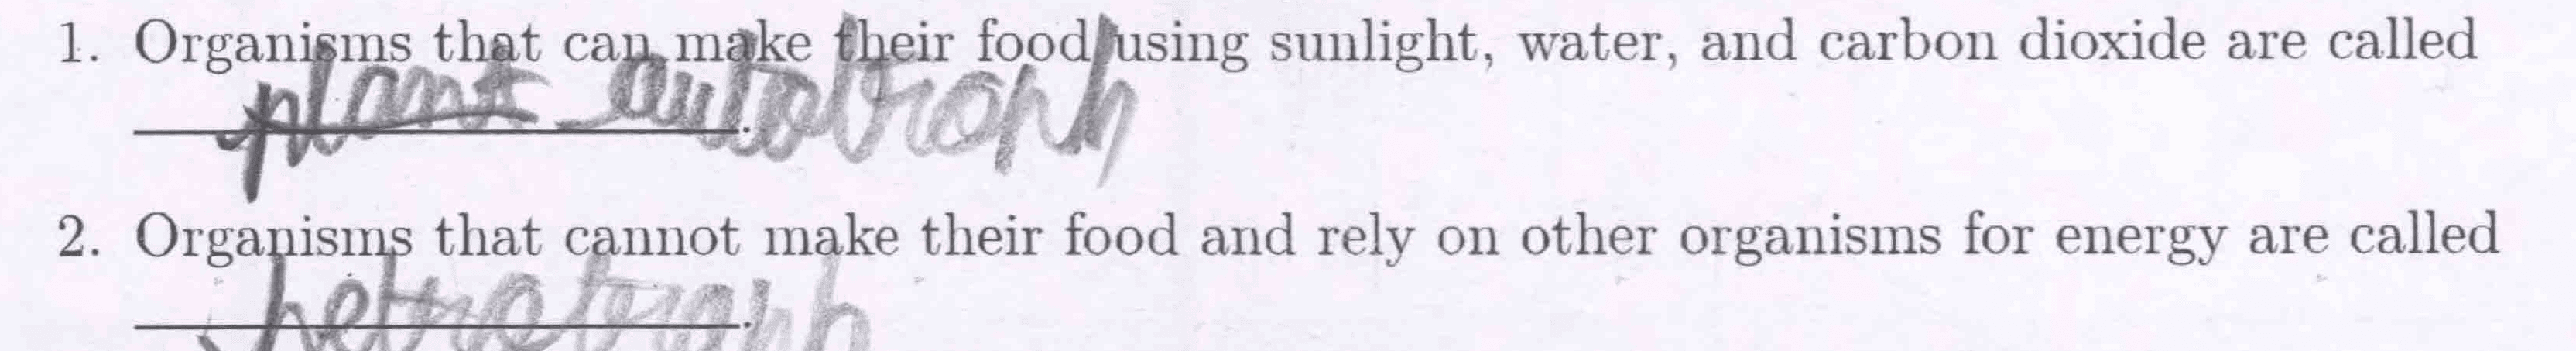
\includegraphics[width=6cm]{Q50_D117198_Science.png}}
    \end{minipage}
    \vspace{10pt}

    % Image: Q50_D117209_Science.png - Scaled height: 2.45mm
    \begin{minipage}{\linewidth}
    \RaggedRight\textbf{\tiny \highgreen{Mahaswetha S [A]}} \\ 
    \vspace{4.00pt}\fcolorbox{blue}{white}{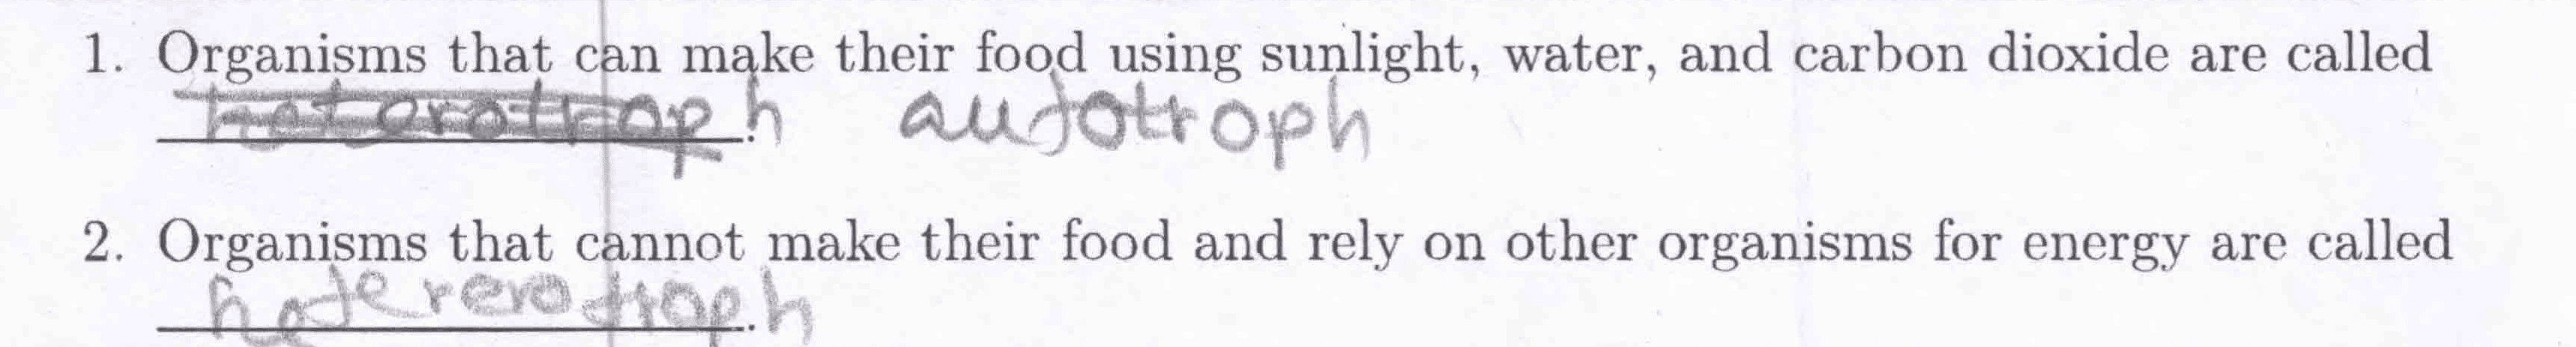
\includegraphics[width=6cm]{Q50_D117209_Science.png}}
    \end{minipage}
    \vspace{10pt}

   
 \end{multicols}
\end{frame}


\begin{frame}[shrink=30,label=QPC7QC7S01 - DT - Q12]{Q57 [1. Nutrition in Plants]}
\vspace{-0.2cm}

\matextbottomTwoTwo{
myanswerquestion={Complete the photosynthesis process based on the given hints.},
myanswercontent={
\tikzset{every picture/.style={line width=0.75pt,scale=\scalefactor}} %set default line width to 0.75pt        

\begin{tikzpicture}[x=0.75pt,y=0.75pt,yscale=-1,xscale=1]
\draw (365.32,149.95) node  {\adjustbox{scale=\scalefactor}{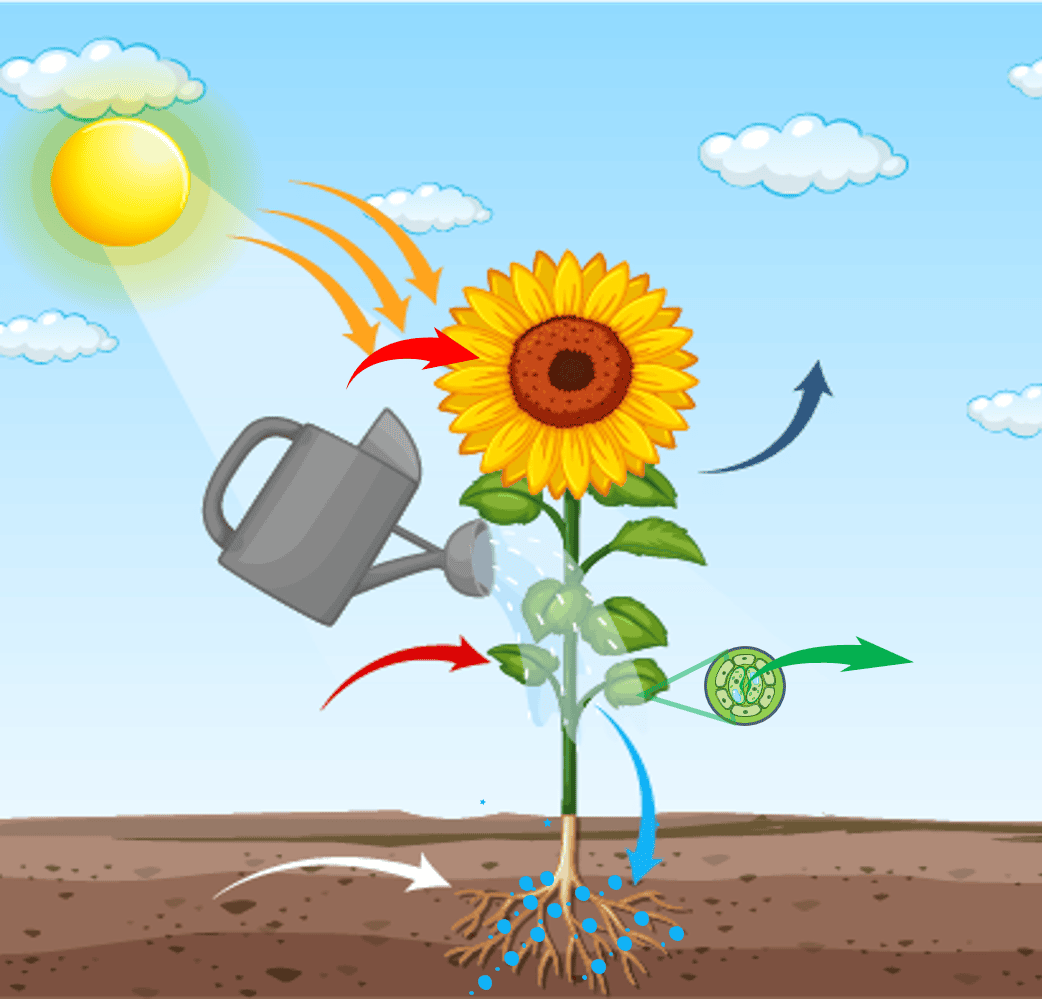
\includegraphics[width=196.5pt,height=188.25pt]{C7S01 - DT - Q12.png}}};
% Text Node
\draw (270,44) node [anchor=north west][inner sep=0.75pt]   [align=left] {Energy source: \rule{100pt}{0.5pt}};
% Text Node
\draw (135,95) node [anchor=north west][inner sep=0.75pt]   [align=left] {End product: Stores energy \\as \rule{100pt}{0.5pt}};
% Text Node
\draw (447,110) node [anchor=north west][inner sep=0.75pt]   [align=left] {Gas released: : \rule{100pt}{0.5pt}};
% Text Node
\draw (75,195) node [anchor=north west][inner sep=0.75pt]   [align=left] {Gas absorbed: \rule{100pt}{0.5pt}};
% Text Node
\draw (471,183) node [anchor=north west][inner sep=0.75pt]   [align=left] {Green pigment \\in leaves: : \rule{100pt}{0.5pt}};
% Text Node
\draw (61,247) node [anchor=north west][inner sep=0.75pt]   [align=left] {Root absorbs: \rule{100pt}{0.5pt}};
\end{tikzpicture}\\
},
questionnumber={57}, 
questionTag={C7S01 - DT - Q12}, 
questiontext={Complete the equation of photosynthesis.\\
\[
\text{Carbon dioxide} + \text{Water} \xrightarrow[\hspace{1cm}\text{?}\hspace{1cm}]{\hspace{1cm}\text{?}\hspace{1cm}} \text{Carbohydrate} + \text{Oxygen}
\] 
},
optionA={Sunlight and stomata},
optionB={Sunlight and chlorophyll},
optionC={Stomata and guard cells},
optionD={Glucose and chlorophyll},
correctoption={B},
}




\begin{minipage}{\linewidth}
\hspace{1cm}
\centering
\tiny
\renewcommand{\arraystretch}{1.25}
\begin{tabular}{|M{1.2cm}|M{0.8cm}|M{0.8cm}|M{0.8cm}|M{0.8cm}|M{0.8cm}|}
\hline
Option & A (\ding{55}) & \cellcolor{cellgreen} B (\ding{51}) & C (\ding{55}) & D (\ding{55}) & E \\ 
\hline
7 A & \highno{25\%} & \highno{56\%} & \highno{19\%} & \highno{0\%} & \highno{0\%} \\ 
 \hline 
7 B & \highno{21\%} & \highno{64\%} & \highno{0\%} & \highno{14\%} & \highno{0\%} \\ \hline
\end{tabular}
\end{minipage}

\end{frame}
\begin{frame}{Q57 - My Answer Responses}
    \vspace{-0.6cm}
    \begin{multicols}{3}

    % Image: Q57_D117187_Science.png - Scaled height: 7.21mm
    \begin{minipage}{\linewidth}
    \RaggedRight\textbf{\tiny \highred{Aadhana S S [A]}} \\ 
    \vspace{4.00pt}\fcolorbox{blue}{white}{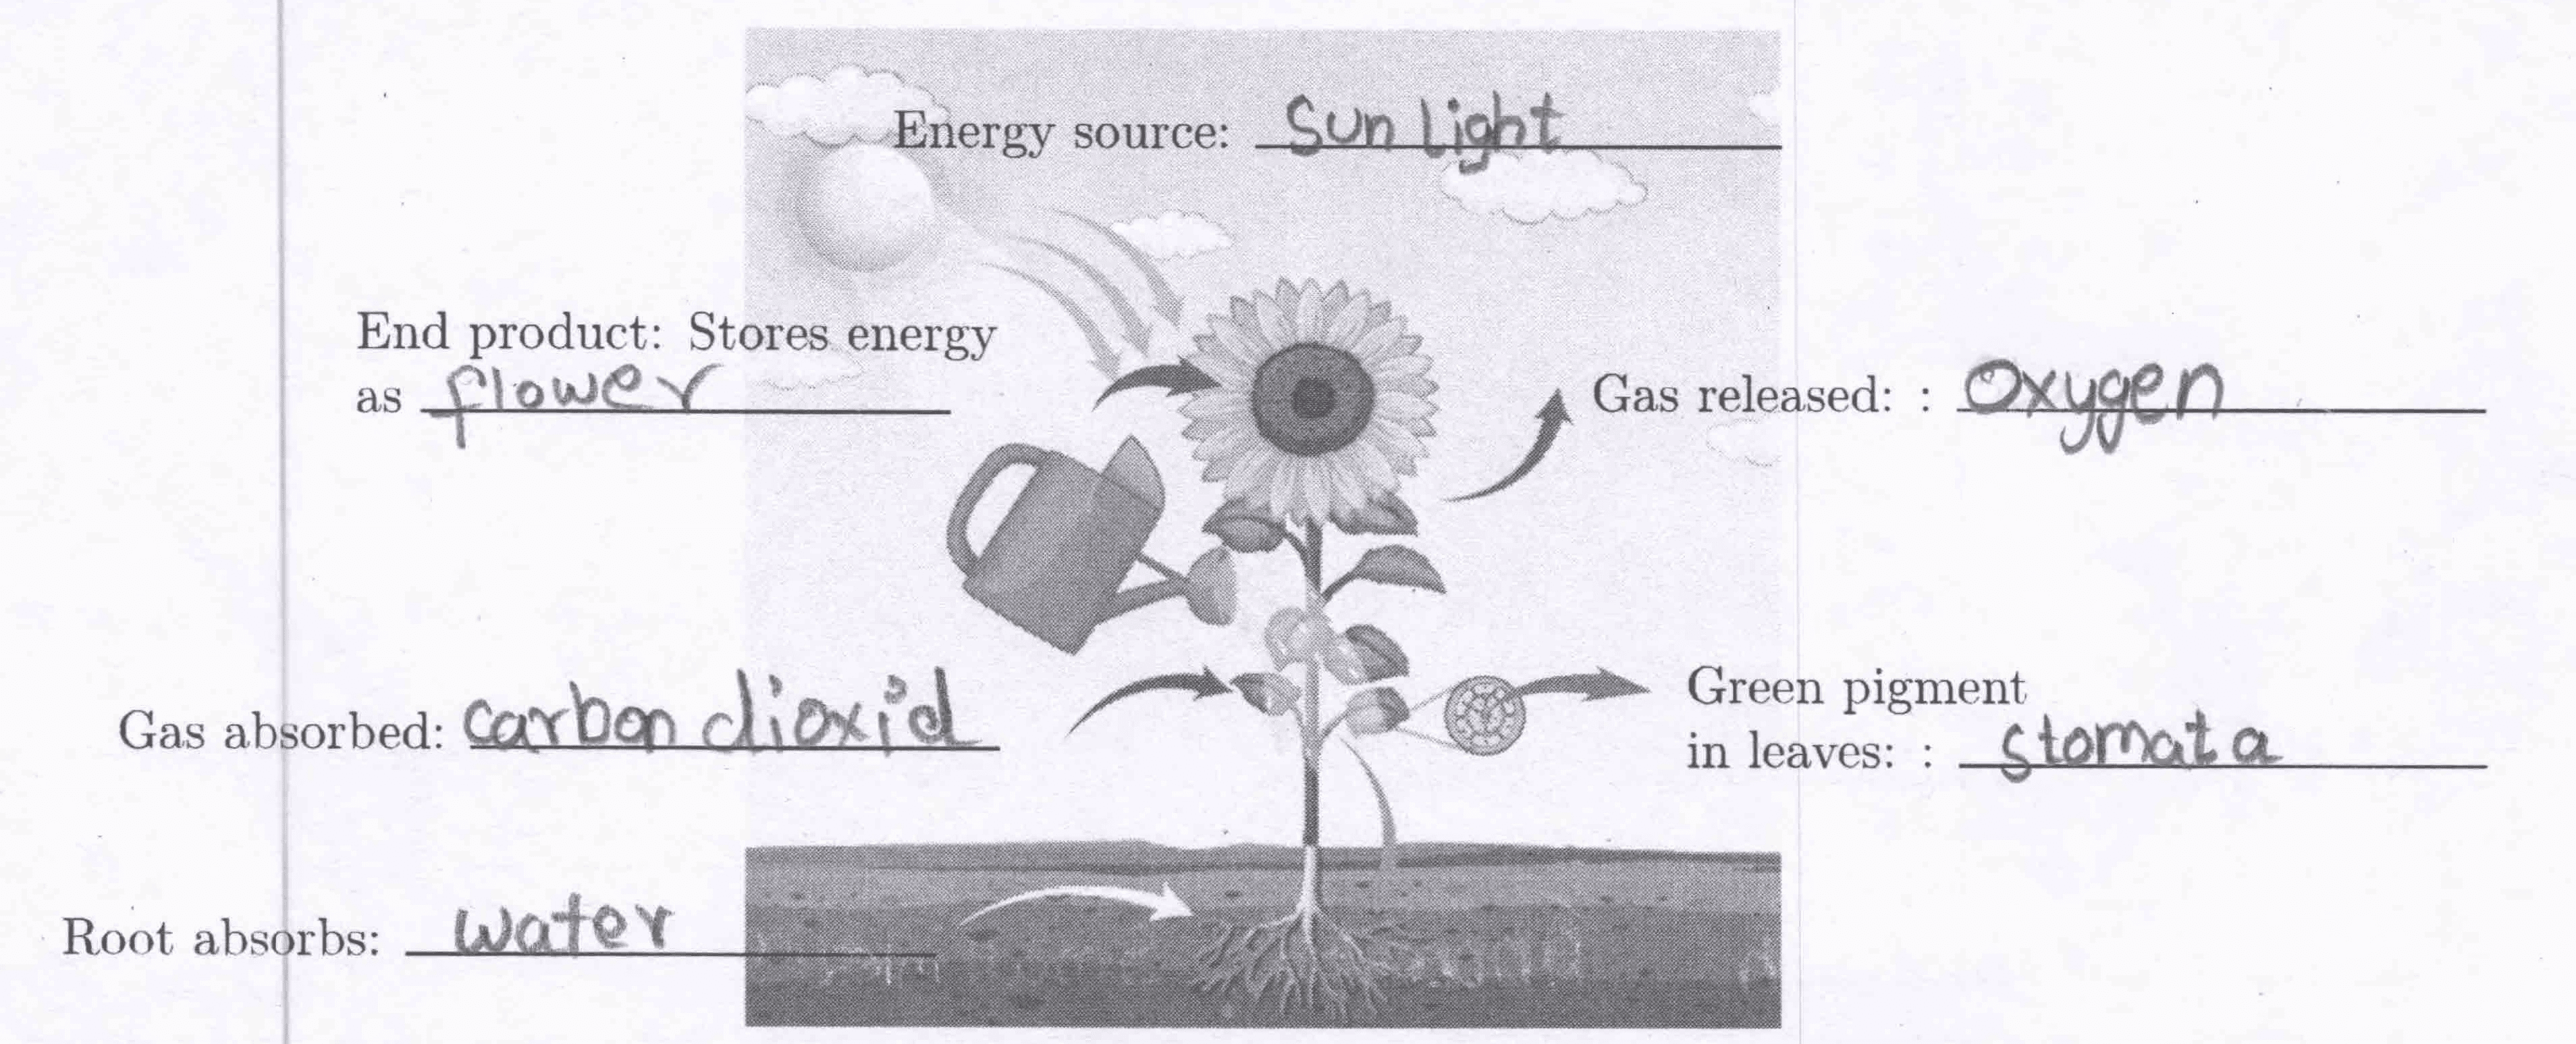
\includegraphics[width=4cm]{Q57_D117187_Science.png}}
    \end{minipage}
    \vspace{10pt}

    % Image: Q57_D117189_Science.png - Scaled height: 6.57mm
    \begin{minipage}{\linewidth}
    \RaggedRight\textbf{\tiny \highgreen{Geetha Deetshana A V [B]}} \\ 
    \vspace{4.00pt}\fcolorbox{blue}{white}{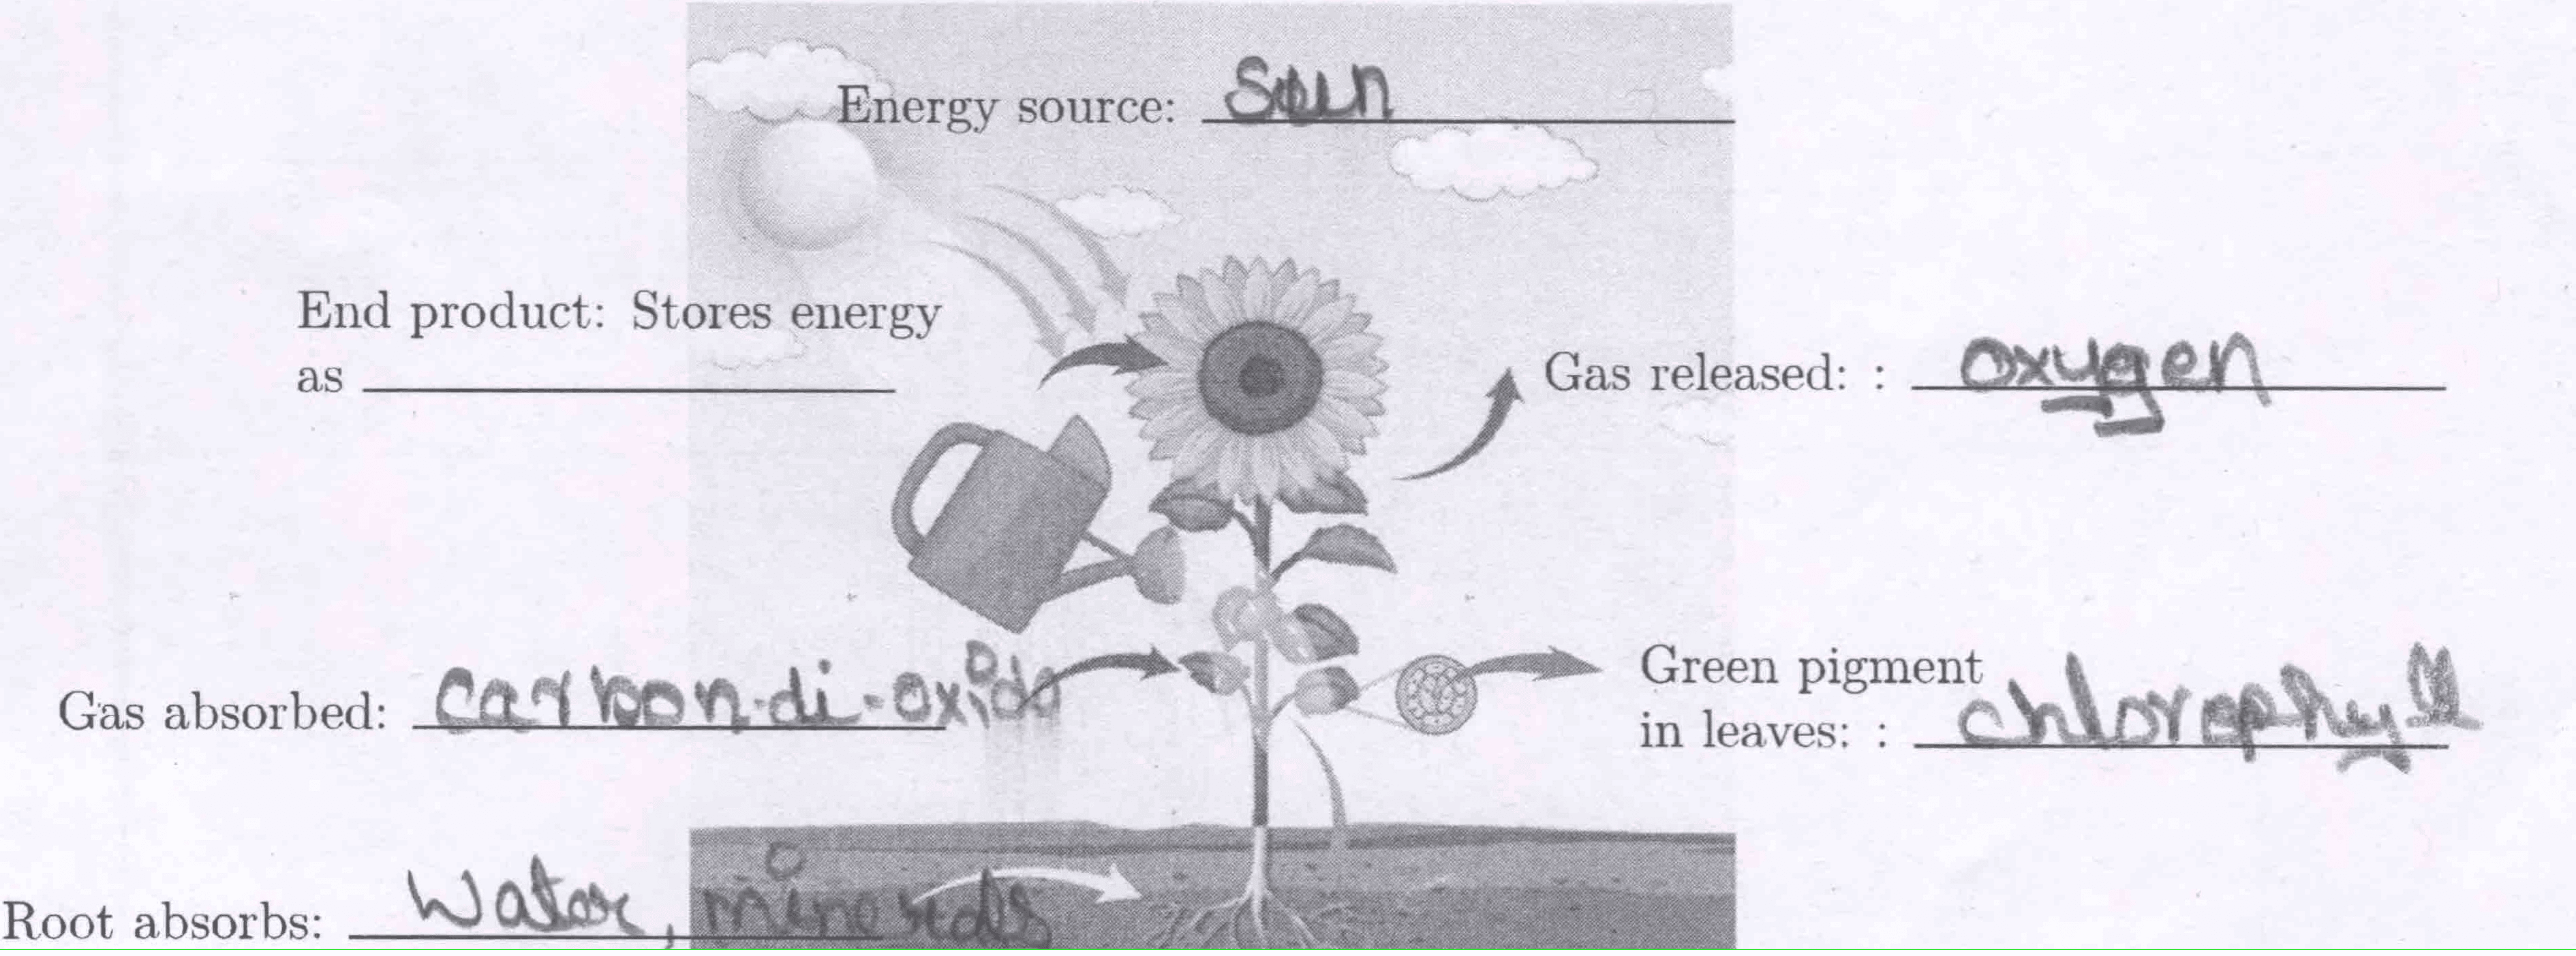
\includegraphics[width=4cm]{Q57_D117189_Science.png}}
    \end{minipage}
    \vspace{10pt}

    % Image: Q57_D117191_Science.png - Scaled height: 7.25mm
    \begin{minipage}{\linewidth}
    \RaggedRight\textbf{\tiny \highgreen{Sharlin Maria T [B]}} \\ 
    \vspace{4.00pt}\fcolorbox{blue}{white}{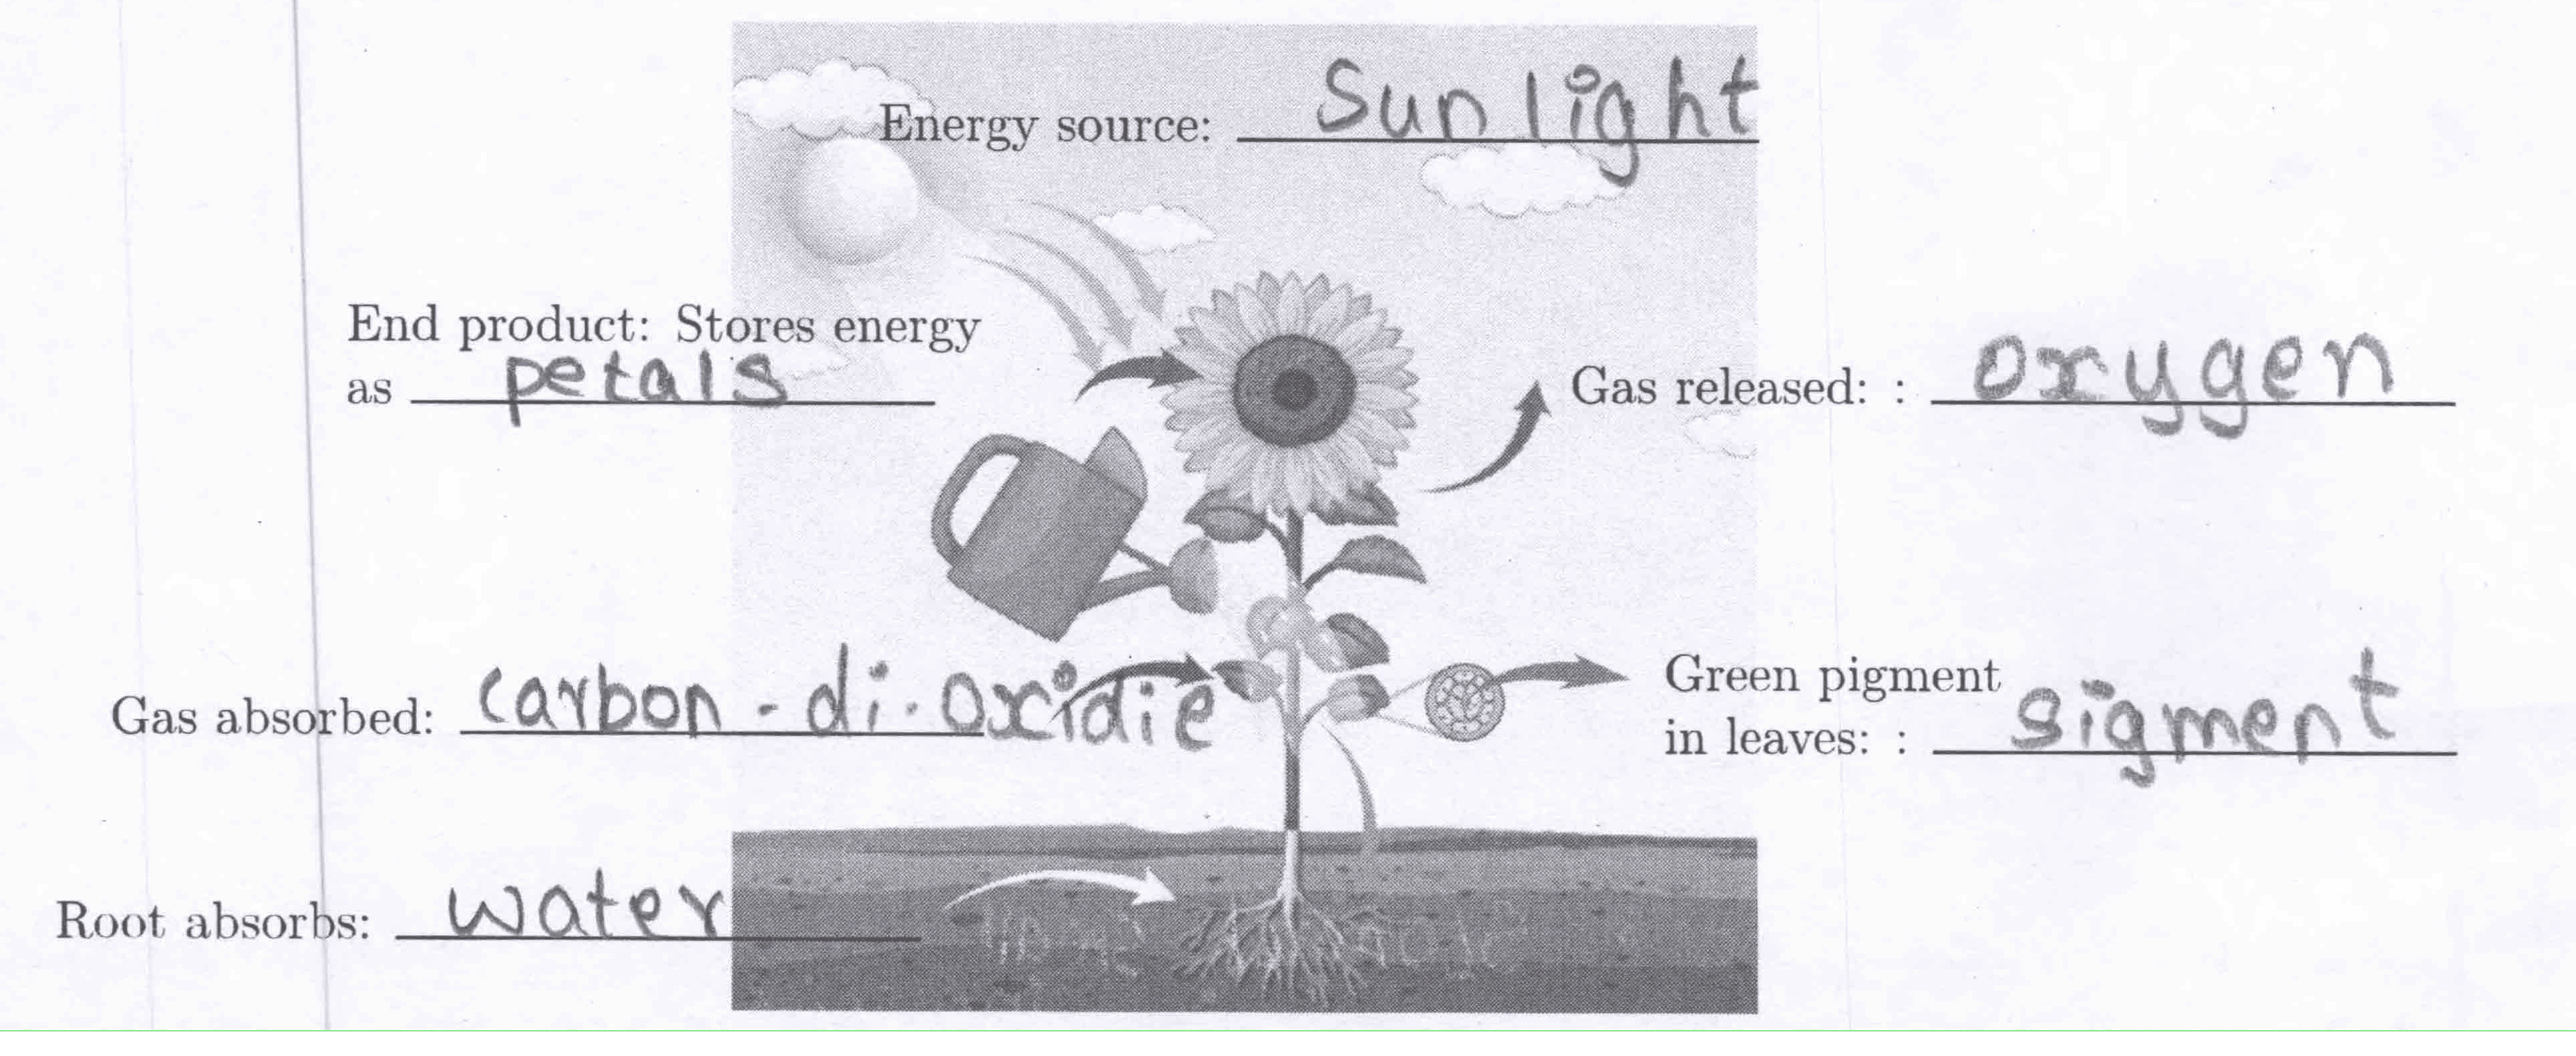
\includegraphics[width=4cm]{Q57_D117191_Science.png}}
    \end{minipage}
    \vspace{10pt}

    % Image: Q57_D117194_Science.png - Scaled height: 6.94mm
    \begin{minipage}{\linewidth}
    \RaggedRight\textbf{\tiny \highred{Tharsika S [C]}} \\ 
    \vspace{4.00pt}\fcolorbox{blue}{white}{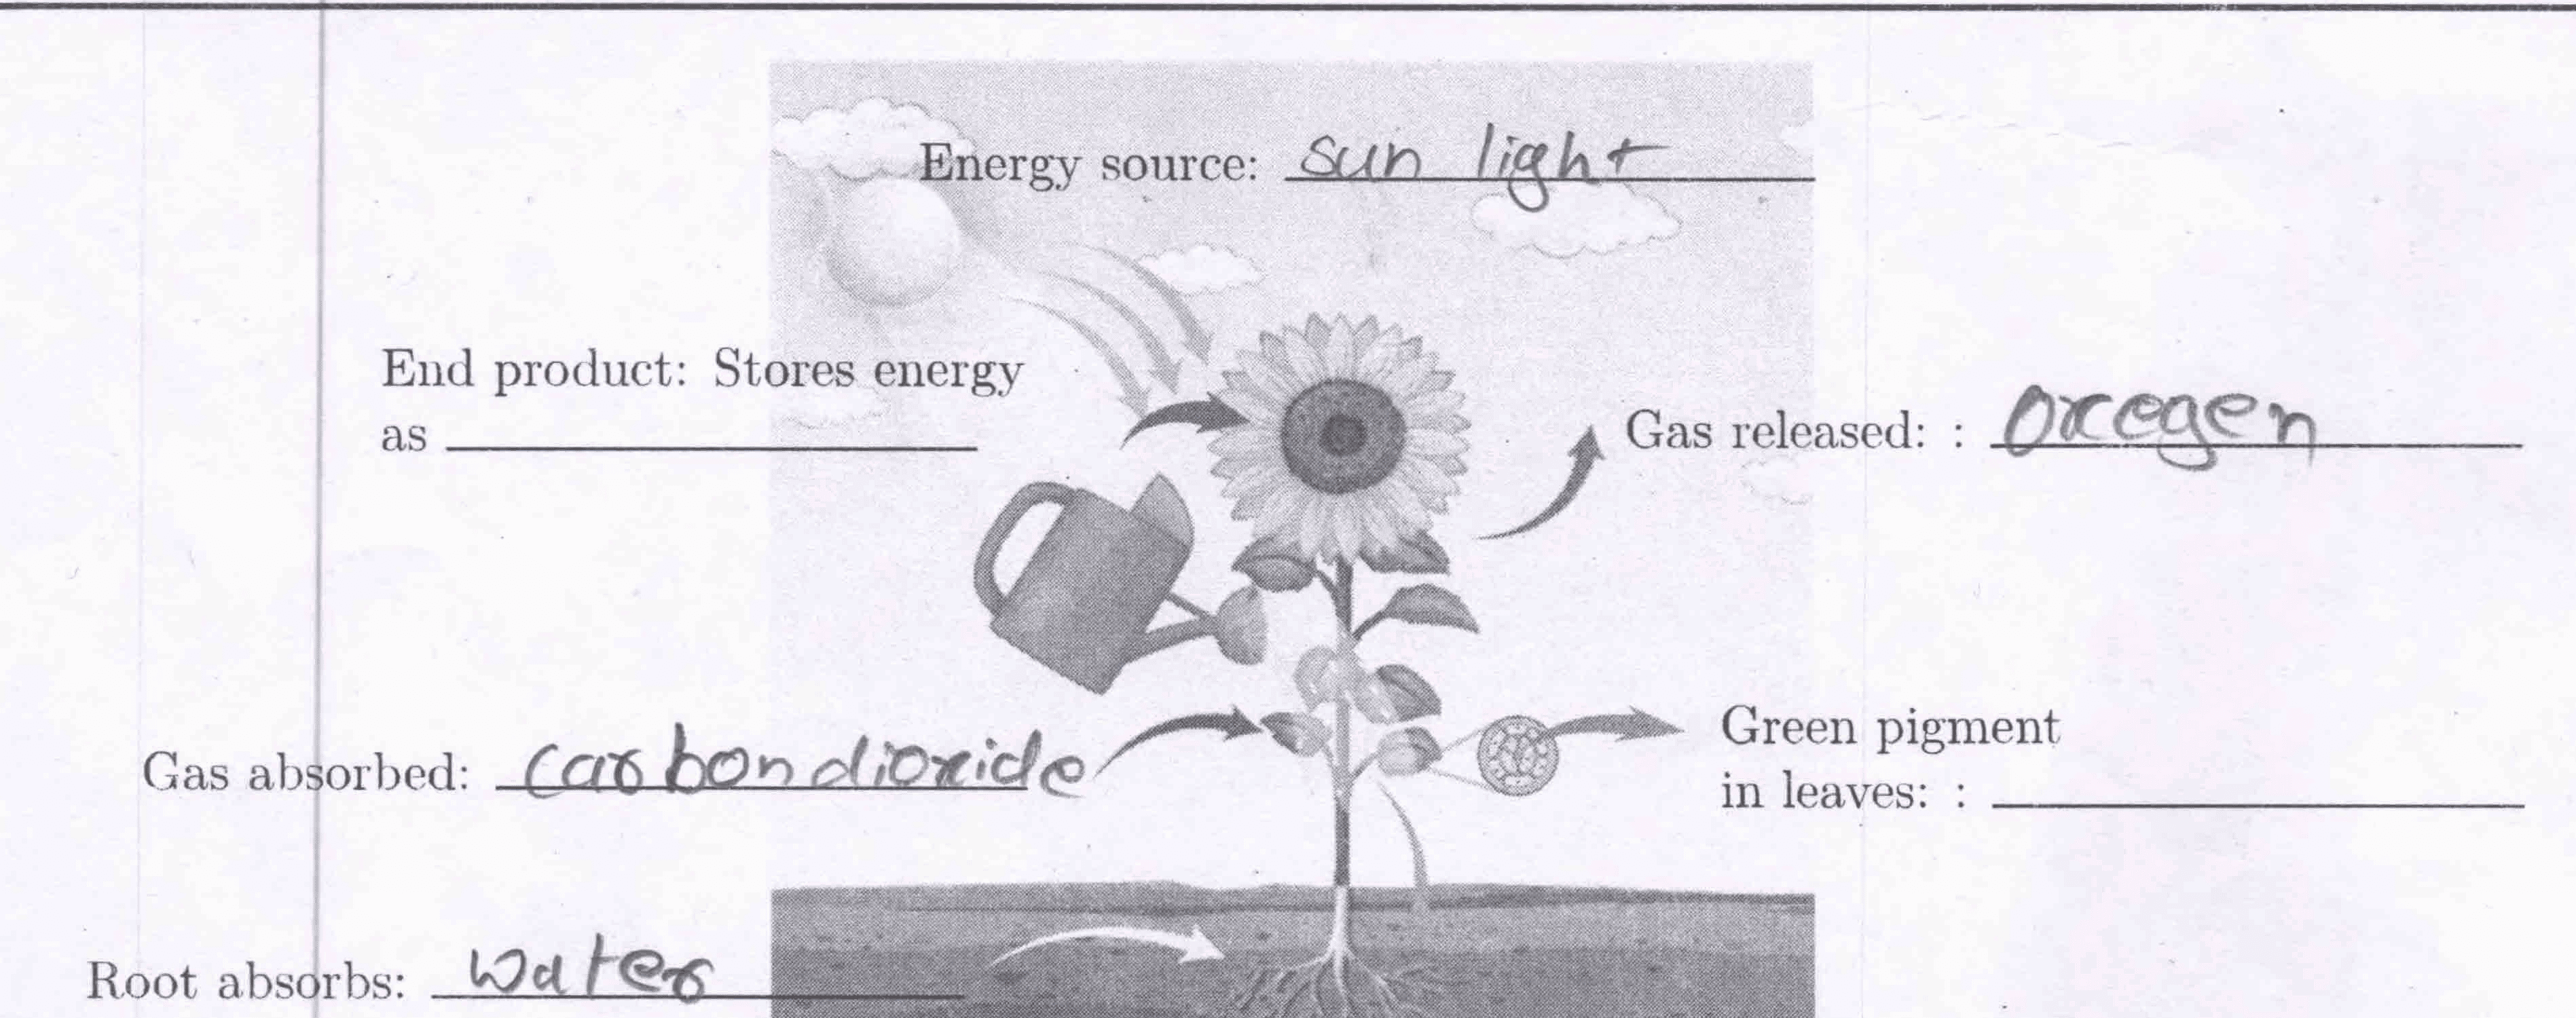
\includegraphics[width=4cm]{Q57_D117194_Science.png}}
    \end{minipage}
    \vspace{10pt}

 
    % Image: Q57_D117203_Science.png - Scaled height: 7.22mm
    \begin{minipage}{\linewidth}
    \RaggedRight\textbf{\tiny \highgreen{Vibin A [B]}} \\ 
    \vspace{4.00pt}\fcolorbox{blue}{white}{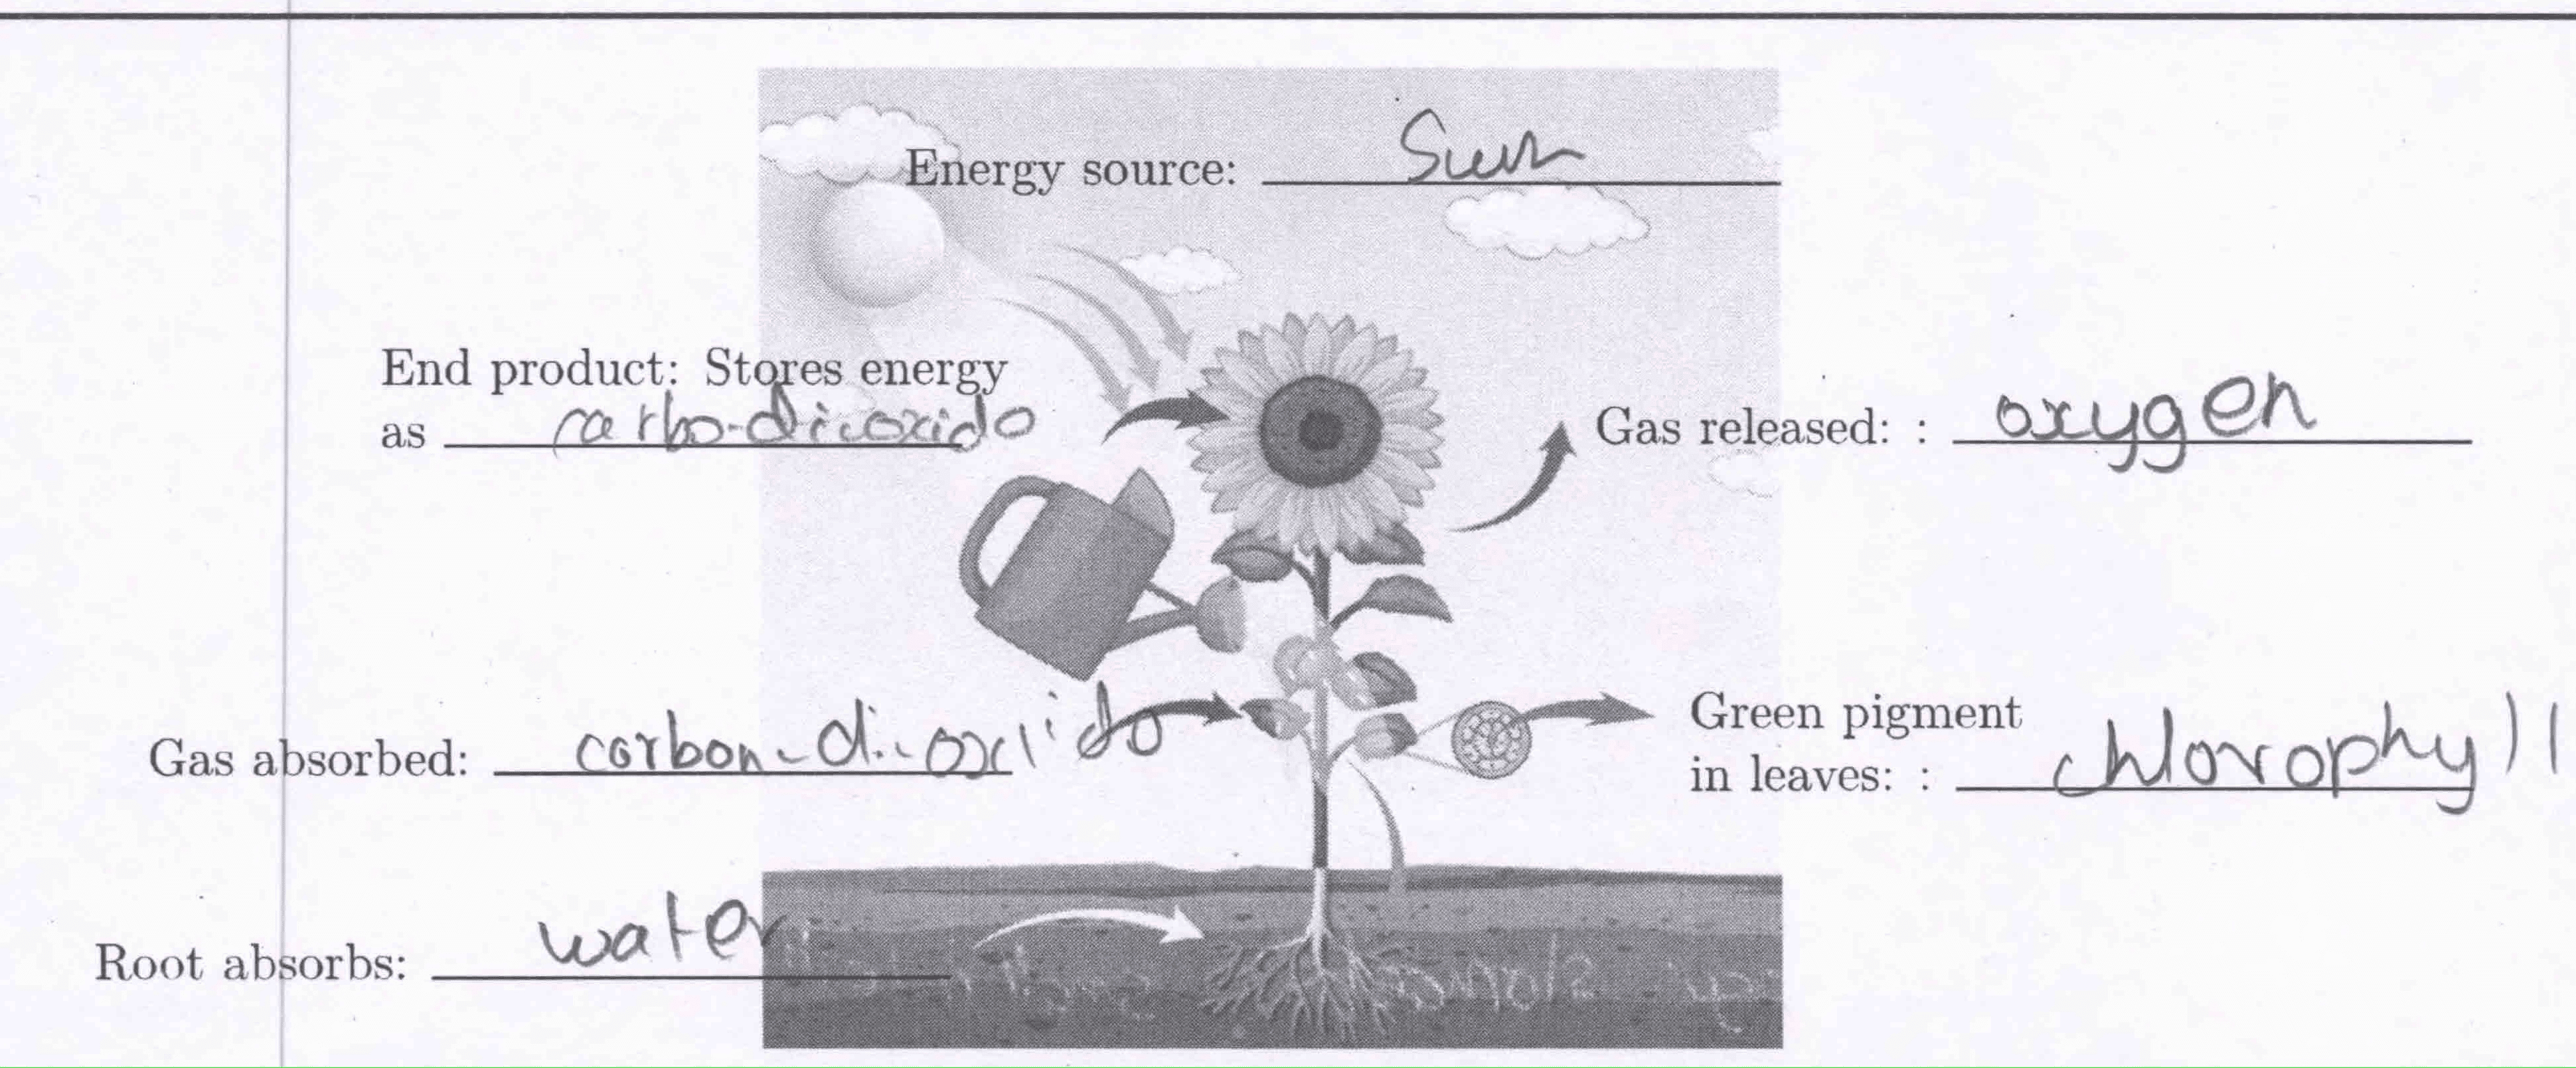
\includegraphics[width=4cm]{Q57_D117203_Science.png}}
    \end{minipage}
    \vspace{10pt}

    % Image: Q57_D117211_Science.png - Scaled height: 7.12mm
    \begin{minipage}{\linewidth}
    \RaggedRight\textbf{\tiny \highgreen{Tanu Shree R S [B]}} \\ 
    \vspace{4.00pt}\fcolorbox{blue}{white}{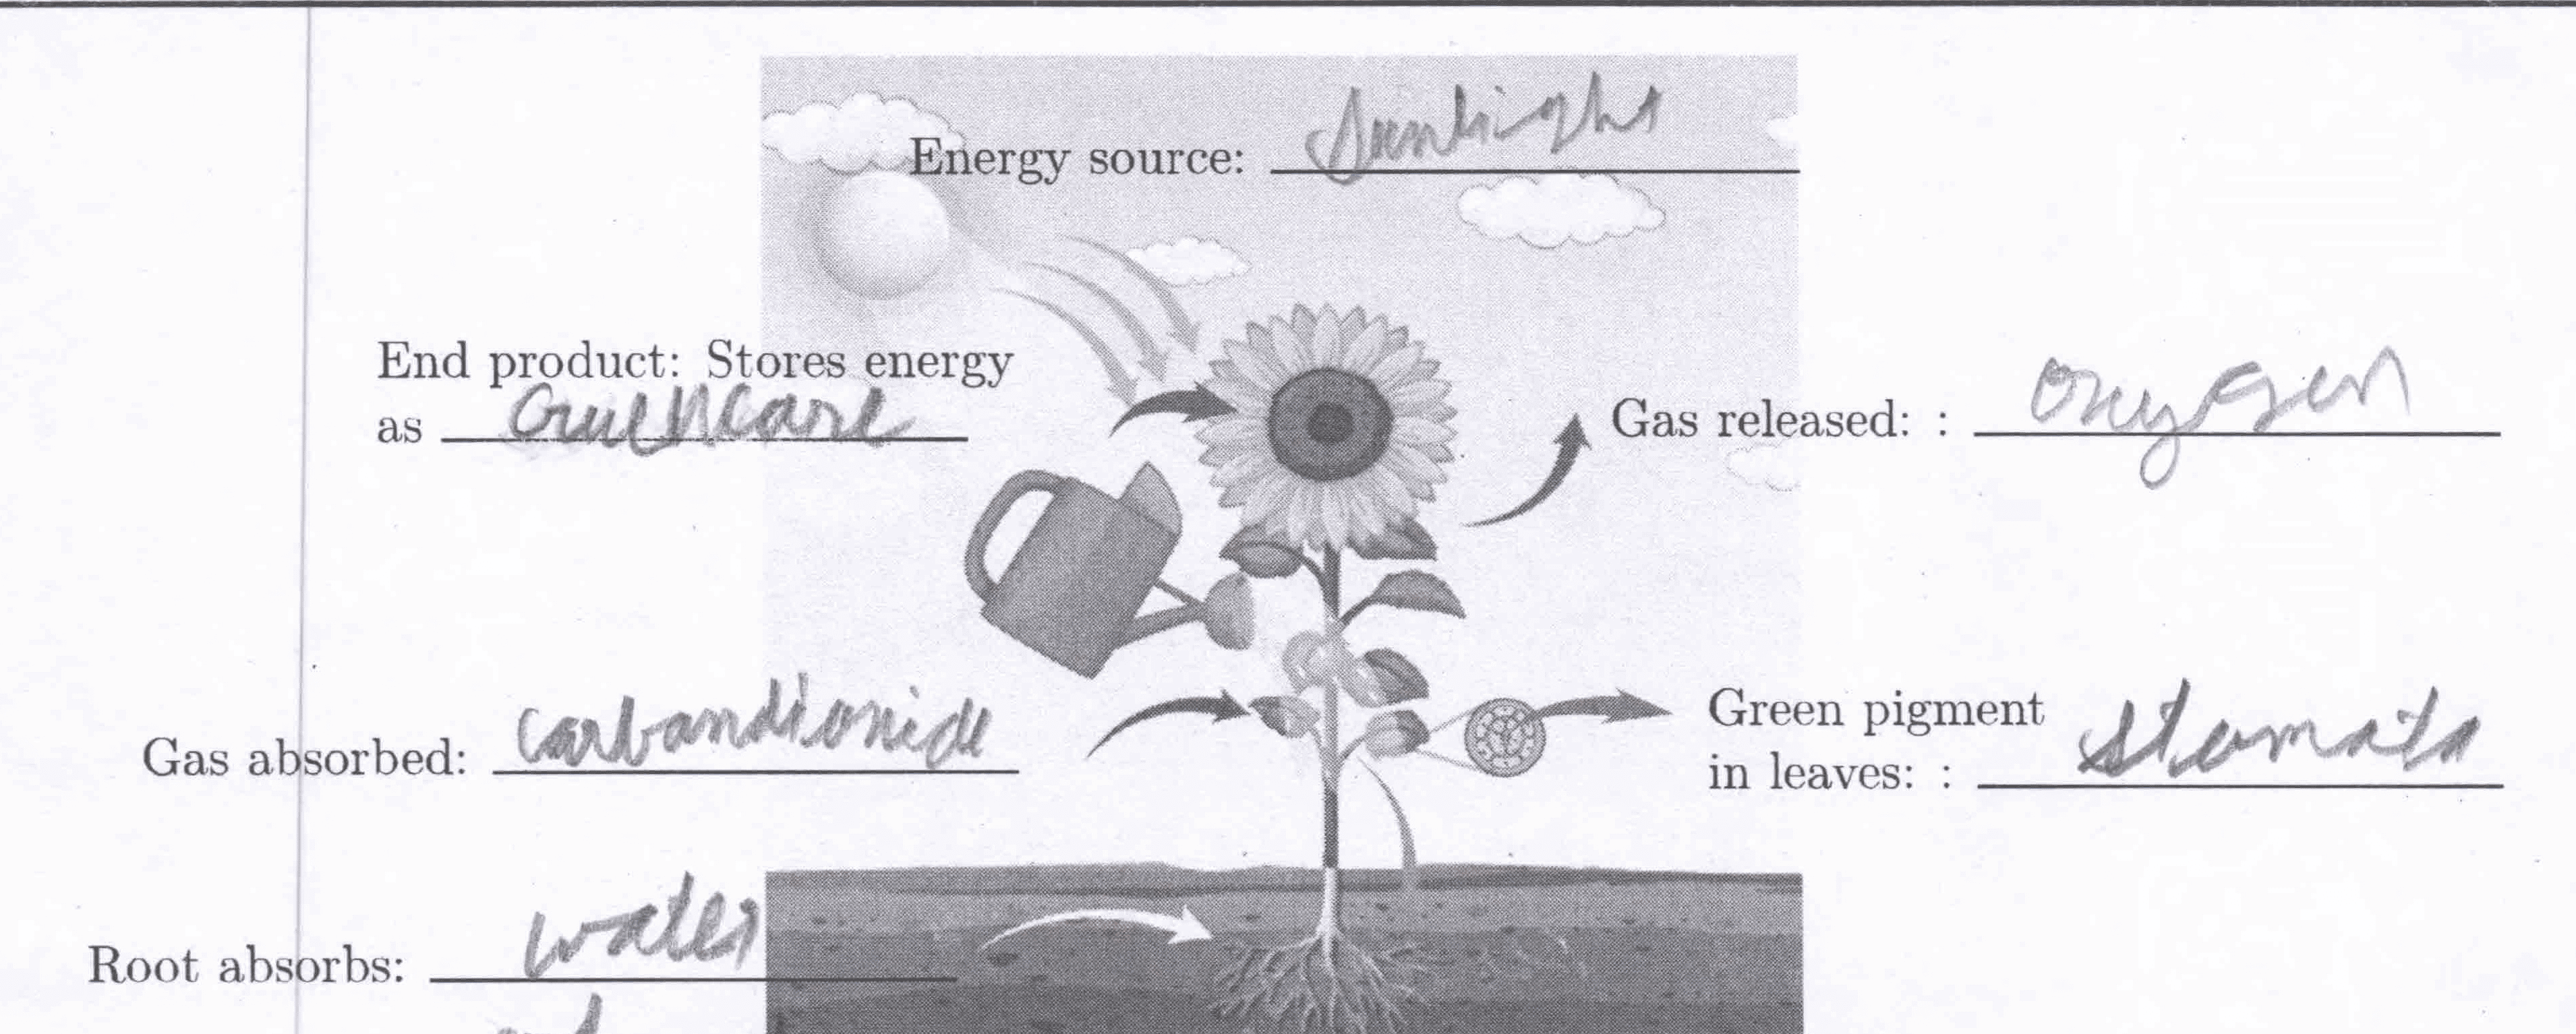
\includegraphics[width=4cm]{Q57_D117211_Science.png}}
    \end{minipage}
    \vspace{10pt}

    \end{multicols}
\end{frame}

\begin{frame}{Q57 - My Answer Responses}
    \vspace{-0.6cm}
    \begin{multicols}{2}

   % Image: Q57_D117197_Science.png - Scaled height: 6.55mm
    \begin{minipage}{\linewidth}
    \RaggedRight\textbf{\tiny \highred{Dharshan K [D]}} \\ 
    \vspace{4.00pt}\fcolorbox{blue}{white}{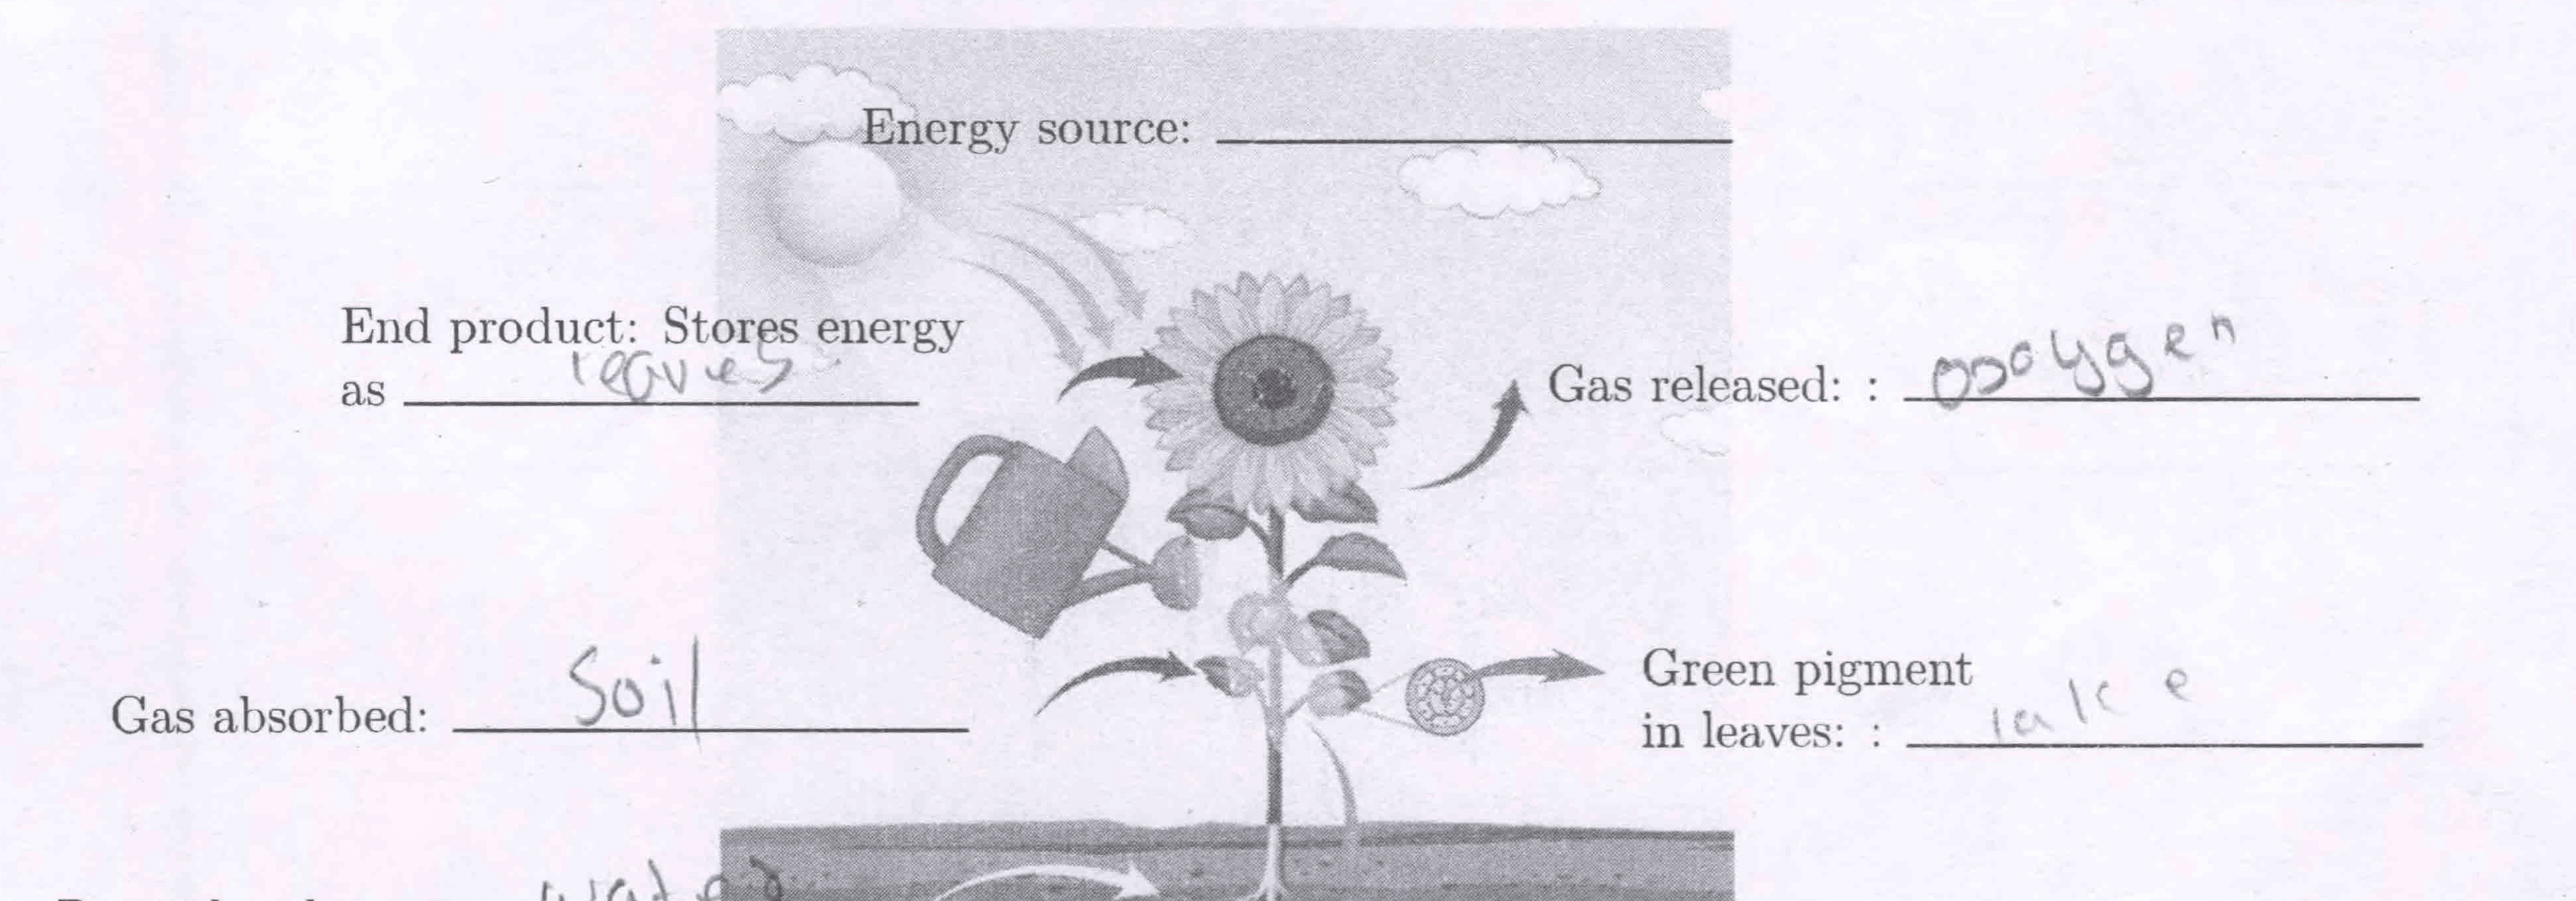
\includegraphics[width=4cm]{Q57_D117197_Science.png}}
    \end{minipage}
    \vspace{10pt}

    % Image: Q57_D117198_Science.png - Scaled height: 7.12mm
    \begin{minipage}{\linewidth}
    \RaggedRight\textbf{\tiny \highgreen{Eniyan E [B]}} \\ 
    \vspace{4.00pt}\fcolorbox{blue}{white}{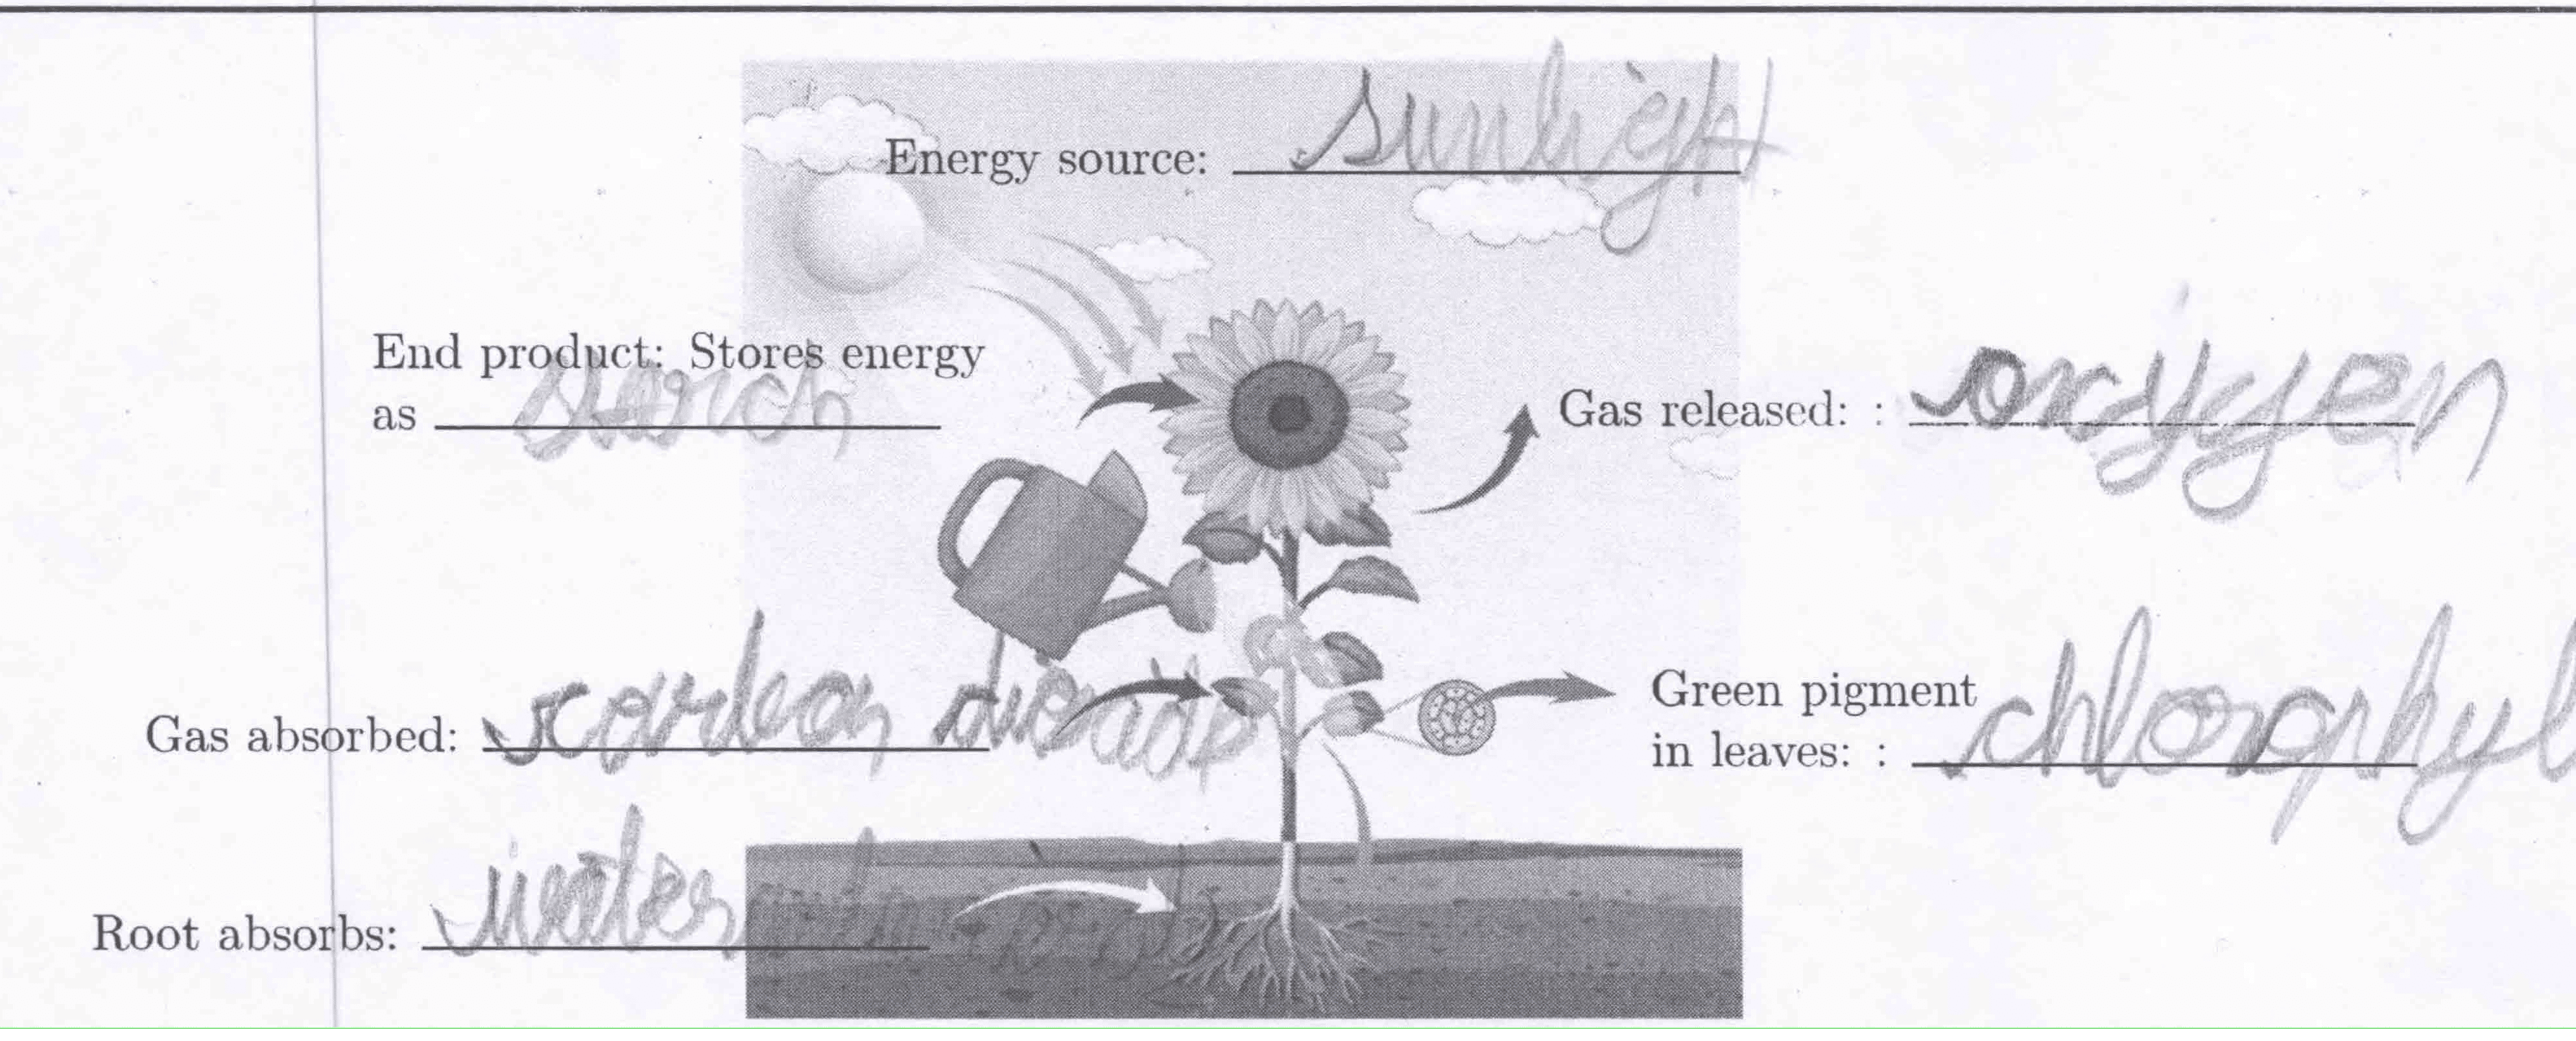
\includegraphics[width=4cm]{Q57_D117198_Science.png}}
    \end{minipage}
    \vspace{10pt}

    % Image: Q57_D117199_Science.png - Scaled height: 7.00mm
    \begin{minipage}{\linewidth}
    \RaggedRight\textbf{\tiny \highgreen{Karthick V [B]}} \\ 
    \vspace{4.00pt}\fcolorbox{blue}{white}{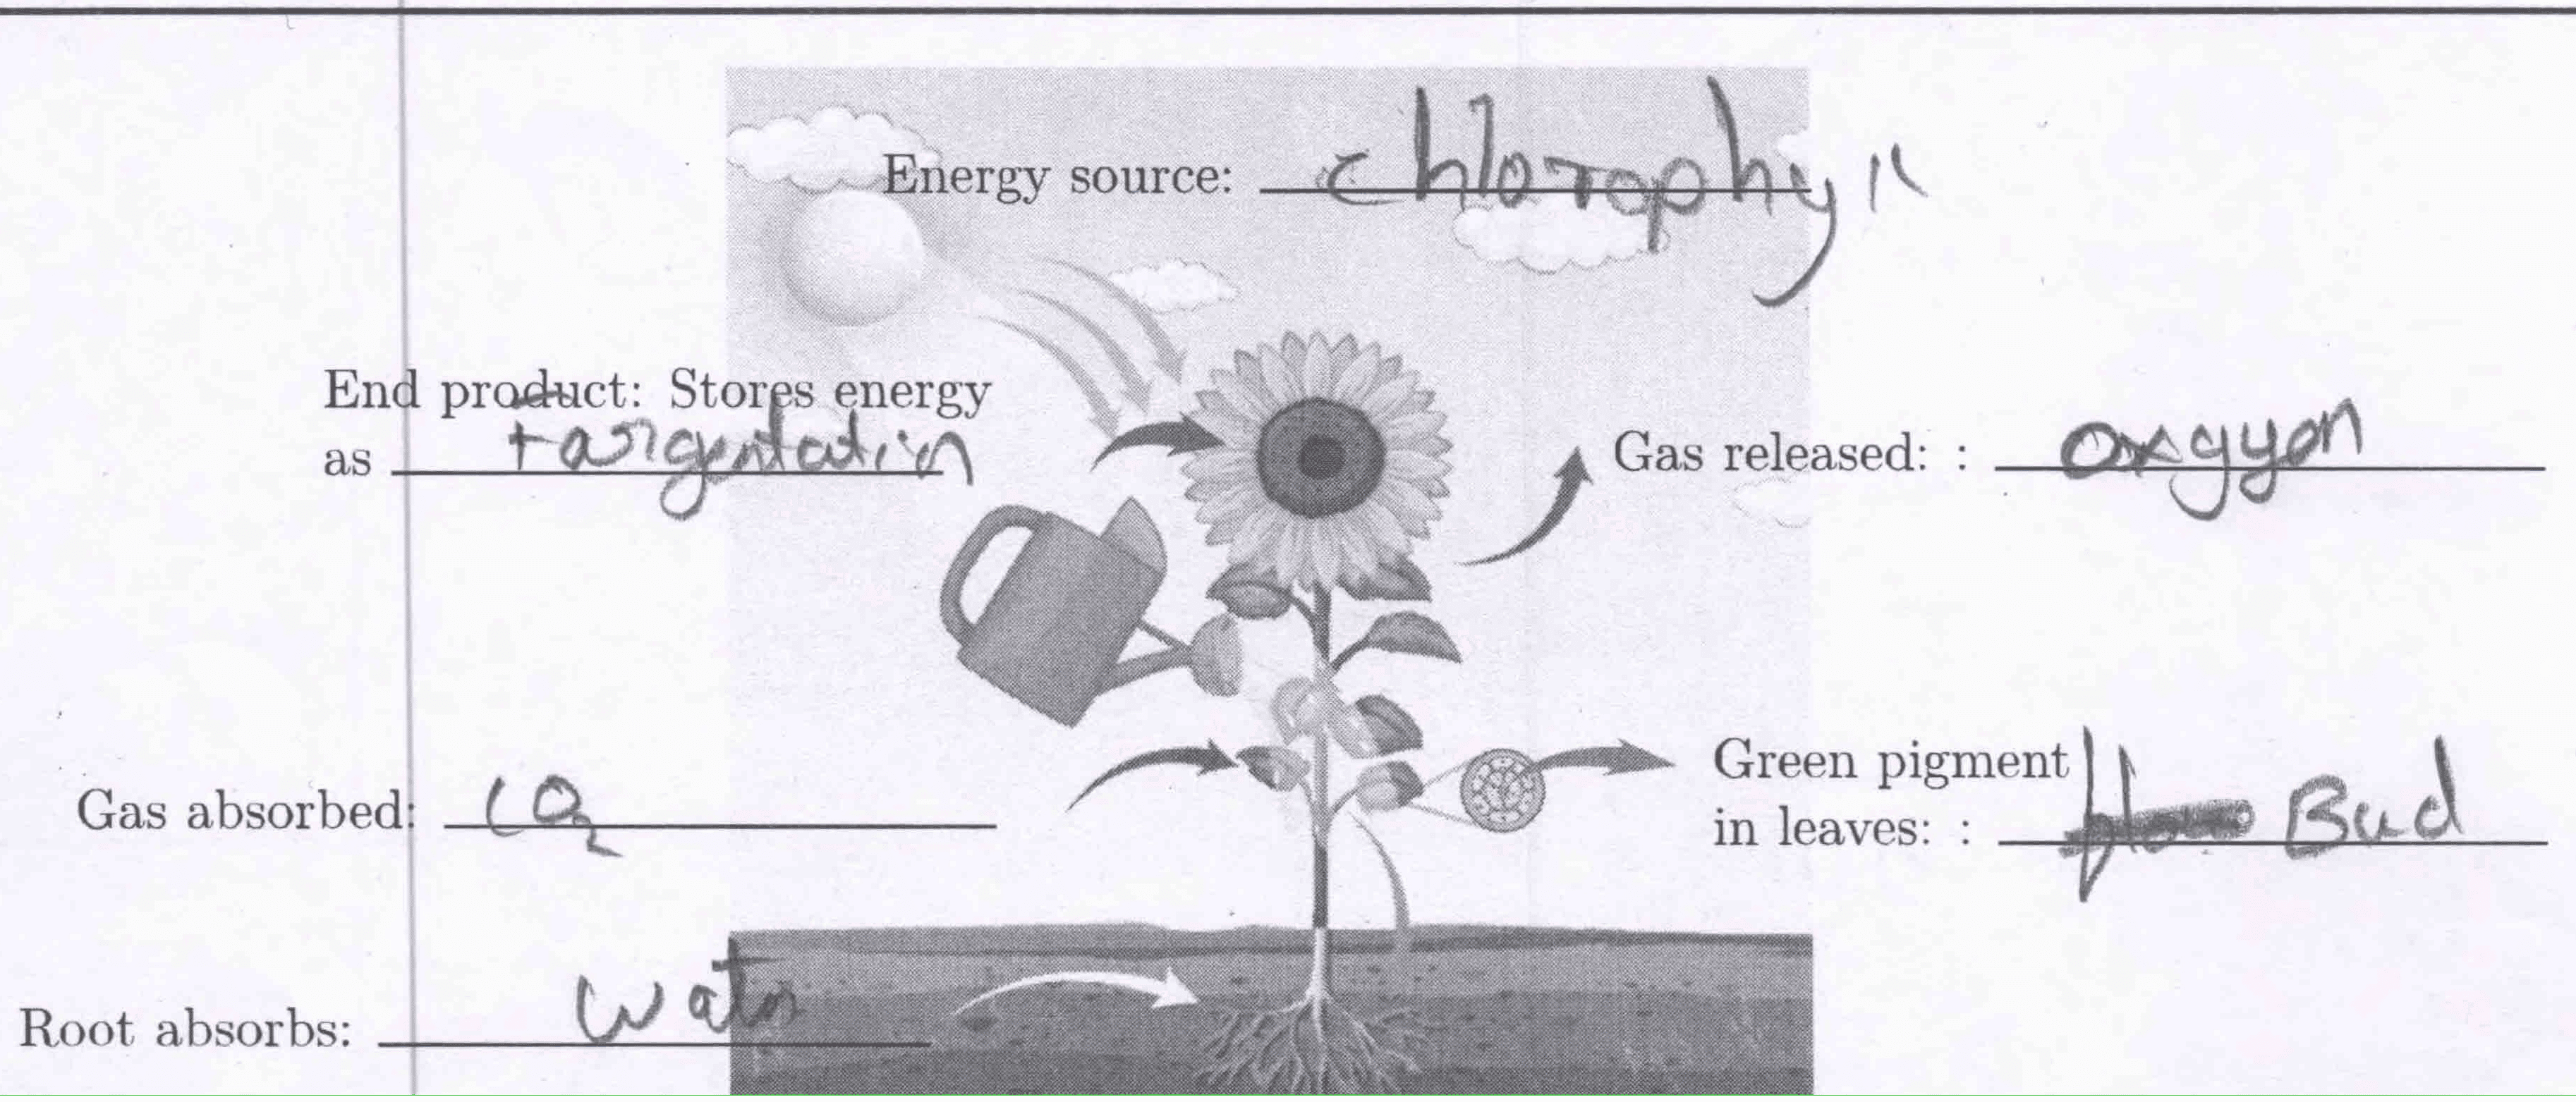
\includegraphics[width=4cm]{Q57_D117199_Science.png}}
    \end{minipage}
    \vspace{10pt}

    % Image: Q57_D117202_Science.png - Scaled height: 7.05mm
    \begin{minipage}{\linewidth}
    \RaggedRight\textbf{\tiny \highgreen{Sashaanth S K [B]}} \\ 
    \vspace{4.00pt}\fcolorbox{blue}{white}{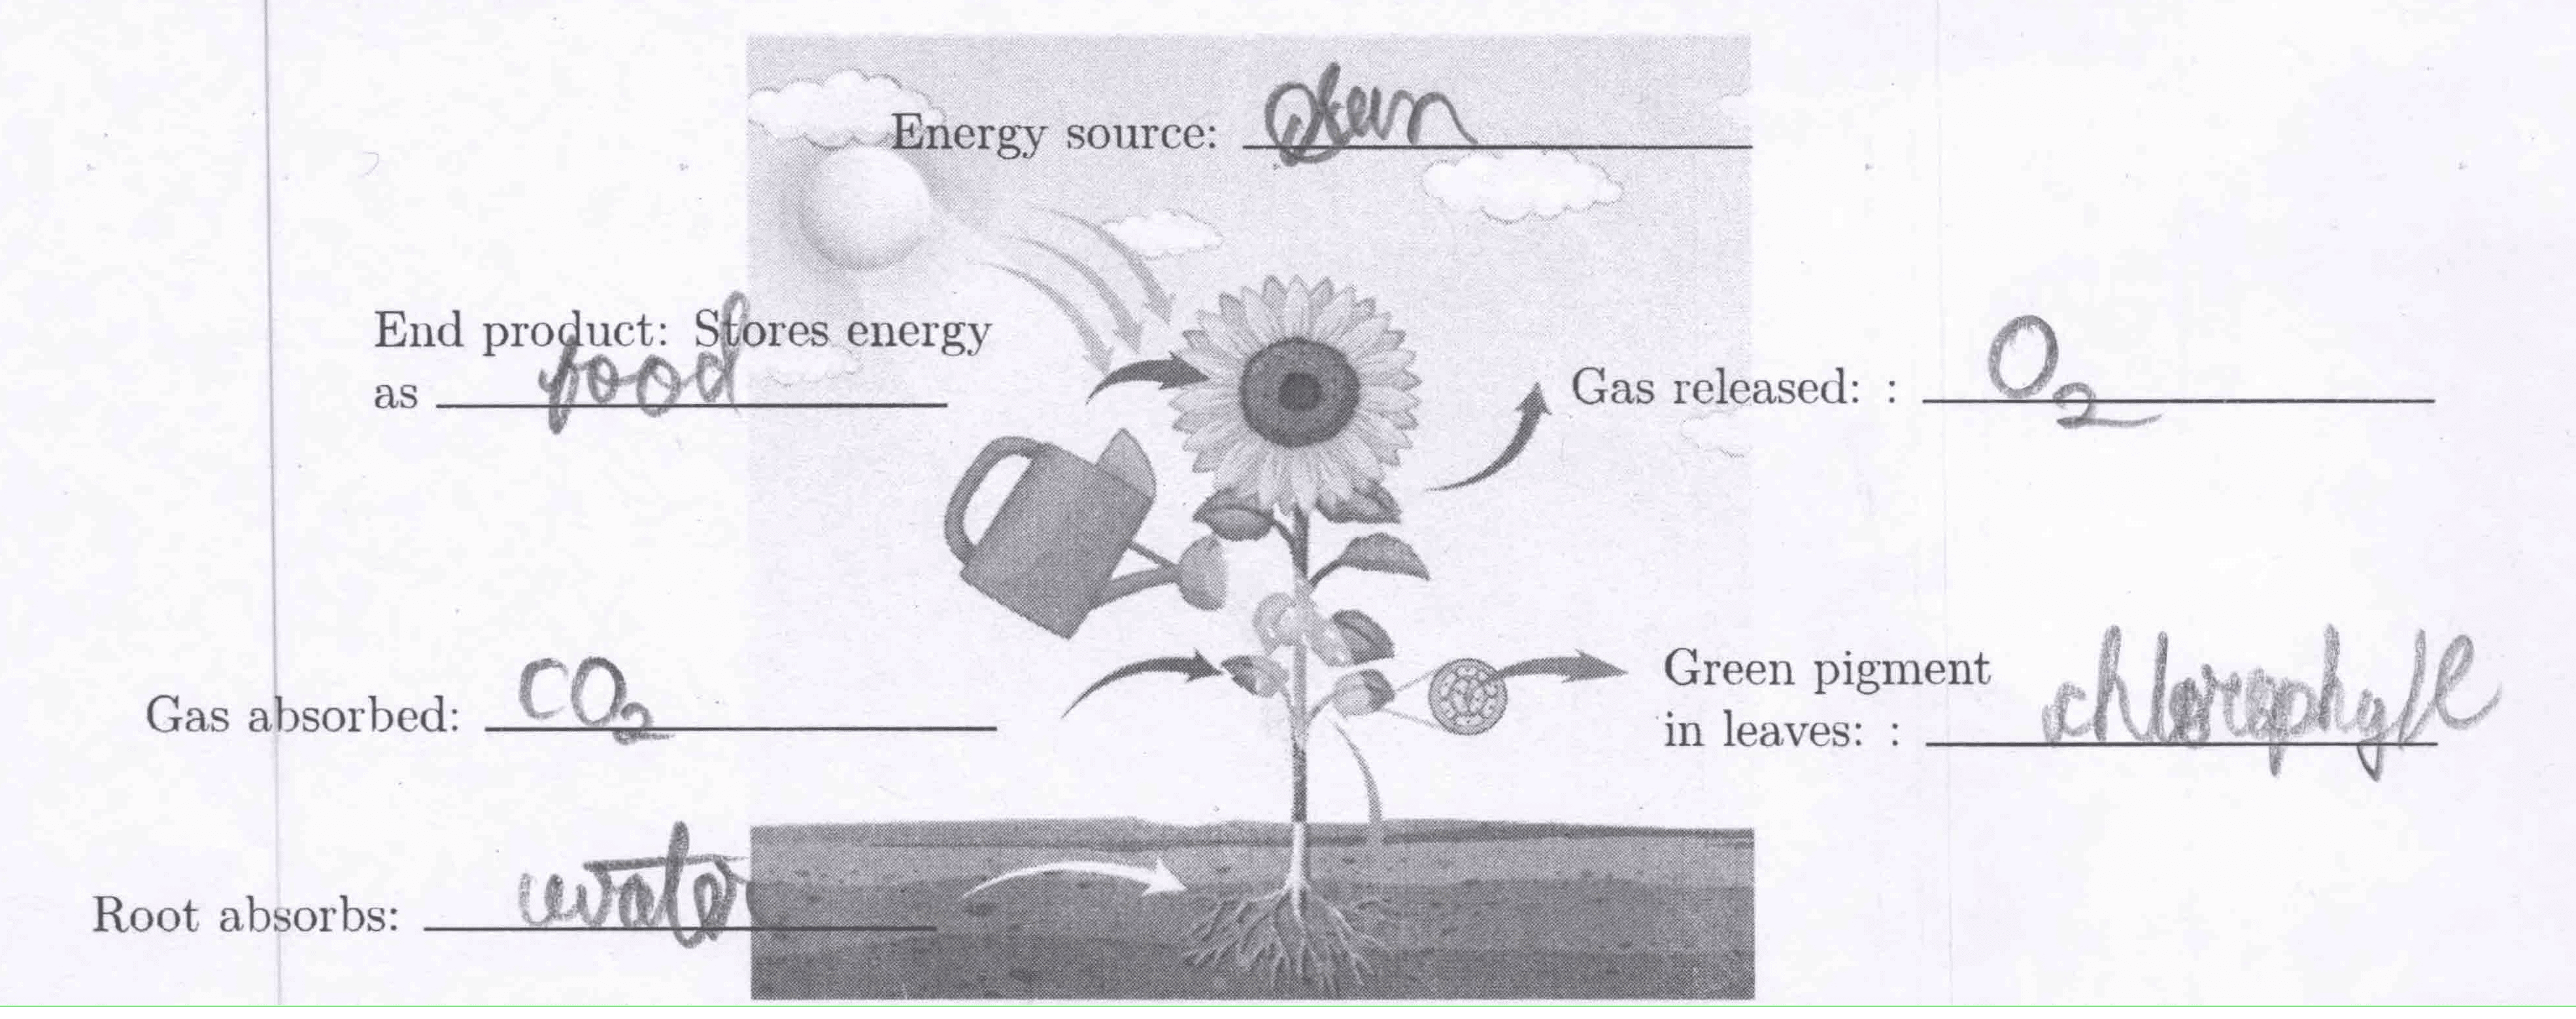
\includegraphics[width=4cm]{Q57_D117202_Science.png}}
    \end{minipage}
    \vspace{10pt}

 \end{multicols}
\end{frame}


\begin{frame}[shrink=0.1,label=QPC7QC7S02 - DT - Q2]{Q8 [2. Nutrition in Animals]}
\vspace{-0.2cm}
\mcqtextbottomOneFour{
  questionnumber={8}, 
  questionTag={C7S02 – DT – Q2}, 
  questiontext={The process of breaking down food from complex substances into simpler substances is called \rule{80pt}{0.1pt}.},
  optionA={Nutrition },
  optionB={Respiration},
  optionC={Digestion},
  optionD={Inhalation},
  correctoption={C},
}

\begin{minipage}{\linewidth}
\hspace{1cm}
\centering
\tiny
\renewcommand{\arraystretch}{1.25}
\begin{tabular}{|M{1.2cm}|M{0.8cm}|M{0.8cm}|M{0.8cm}|M{0.8cm}|M{0.8cm}|}
\hline
Option & A (\ding{55}) & B (\ding{55}) & \cellcolor{cellgreen} C (\ding{51}) & D (\ding{55}) & E \\ 
\hline
7 A & \highno{13\%} & \highno{25\%} & \highno{63\%} & \highno{0\%} & \highno{0\%} \\ 
 \hline 
7 B & \highno{0\%} & \highno{36\%} & \highno{64\%} & \highno{0\%} & \highno{0\%} \\ \hline
\end{tabular}
\end{minipage}

\end{frame}
% \input{4. PPT/6. My Answer/Science/C7/117_C7S - Q8}


\begin{frame}[shrink=0.1,label=QPC7QC7S02 - DT - Q3]{Q10 [2. Nutrition in Animals]}
\vspace{-0.2cm}
\mcqtextbottomTwoTwo{
  questionnumber={10}, 
  questionTag={C7S02 – DT – Q3}, 
  questiontext={Find the incorrect function of the organ found in the buccal cavity or mouth.},
  optionA={Tongue – Identifies the taste of the food. },
  optionB={Teeth – Chew the food.},
  optionC={Saliva – Converts starch into sugar.  },
  optionD={Oesophagus – Secretes saliva. },
  correctoption={D},
}

\begin{minipage}{\linewidth}
\hspace{1cm}
\centering
\tiny
\renewcommand{\arraystretch}{1.25}
\begin{tabular}{|M{1.2cm}|M{0.8cm}|M{0.8cm}|M{0.8cm}|M{0.8cm}|M{0.8cm}|}
\hline
Option & A (\ding{55}) & B (\ding{55}) & C (\ding{55}) & \cellcolor{cellgreen} D (\ding{51}) & E \\ 
\hline
7 A & \highno{6\%} & \highno{19\%} & \highno{6\%} & \highno{69\%} & \highno{0\%} \\ 
 \hline 
7 B & \highno{14\%} & \highno{14\%} & \highno{21\%} & \highno{50\%} & \highno{0\%} \\ \hline
\end{tabular}
\end{minipage}

\end{frame}
% \input{4. PPT/6. My Answer/Science/C7/117_C7S - Q10}


\begin{frame}[shrink=0.1,label=QPC7QC7S02 - DT - Q10]{Q16 [2. Nutrition in Animals]}
\vspace{-0.2cm}
\mcqtextbottomOneFour{
  questionnumber={16}, 
  questionTag={C7S02 – DT – Q10}, 
  questiontext={Pick the organ that helps in capturing the food in the amoeba.},
  optionA={Nucleus},
  optionB={Pseudopodia},
  optionC={Food vacuole},
  optionD={Cytoplasm},
  correctoption={B},
}

\begin{minipage}{\linewidth}
\hspace{1cm}
\centering
\tiny
\renewcommand{\arraystretch}{1.25}
\begin{tabular}{|M{1.2cm}|M{0.8cm}|M{0.8cm}|M{0.8cm}|M{0.8cm}|M{0.8cm}|}
\hline
Option & A (\ding{55}) & \cellcolor{cellgreen} B (\ding{51}) & C (\ding{55}) & D (\ding{55}) & E \\ 
\hline
7 A & \highno{0\%} & \highred{19\%} & \highno{75\%} & \highno{6\%} & \highno{0\%} \\ 
 \hline 
7 B & \highno{0\%} & \highred{0\%} & \highno{93\%} & \highno{7\%} & \highno{0\%} \\ \hline
\end{tabular}
\end{minipage}

\end{frame}
% \input{4. PPT/6. My Answer/Science/C7/117_C7S - Q16}


\begin{frame}[shrink=0.1,label=QPC7QC7S02 - DT - Q11]{Q60 [2. Nutrition in Animals]}
\vspace{-0.2cm}

\maimgleftFourOne{
myanswerquestion={Arrange the following parts of the digestive system in the correct sequence as food travels through the body, from ingestion to egestion.},
myanswercontent={\renewcommand{\arraystretch}{1.25}
\begin{tabular}{|cccccc|}
\hline
Stomach & Large Intestine & Oesophagus & Mouth & Small Intestine & Anus \\
\hline
\end{tabular} \\
\vspace{0.5cm}
\rule{50pt}{0.5pt} $\rightarrow$ 
\rule{50pt}{0.5pt} $\rightarrow$ 
\rule{50pt}{0.5pt} $\rightarrow$ 
\rule{50pt}{0.5pt}  $\rightarrow$ 
\underline{\textbf{Large intestine}} $\rightarrow$ 
\rule{50pt}{0.5pt}
\\},
questionnumber={60}, 
questionTag={C7S02 - DT - Q11},
questiontext={Look at the image and identify the part of the digestive system where egestion occurs.},
imgtabletikz= {
\tikzset{every picture/.style={line width=0.75pt,scale=\scalefactor}} %set default line width to 0.75pt        
\begin{tikzpicture}[x=0.75pt,y=0.75pt,yscale=-1,xscale=1]
%uncomment if require: \path (0,300); %set diagram left start at 0, and has height of 300
%Image [id:dp9152420065645179] 
\draw (101.67,93.96) node  {\adjustbox{scale=\scalefactor}{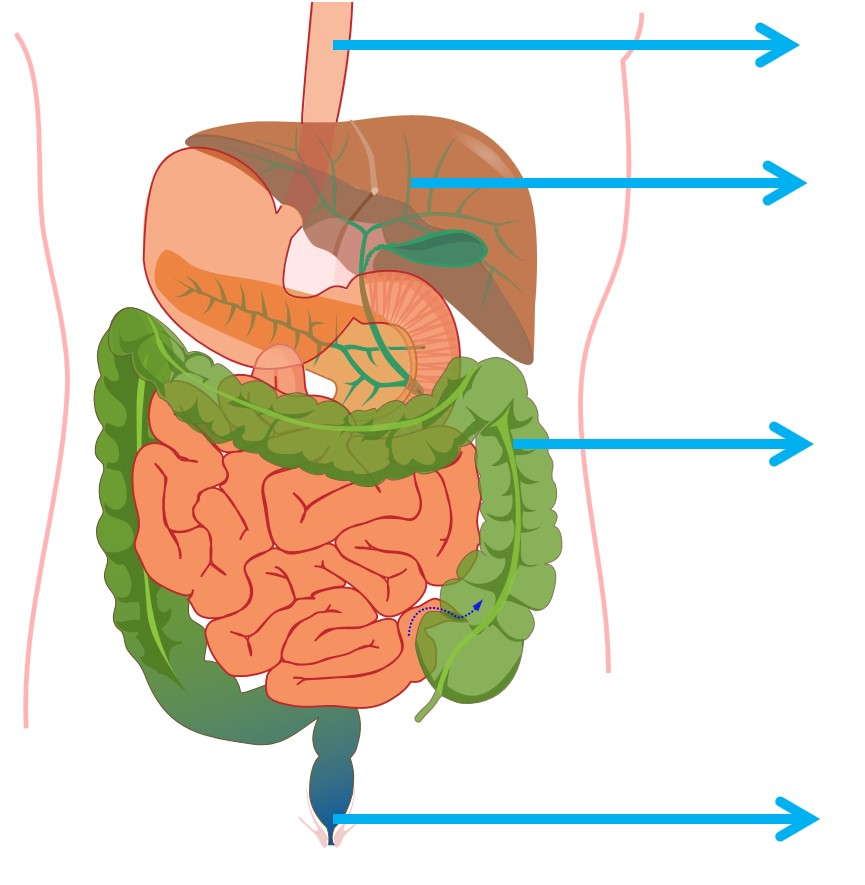
\includegraphics[width=86.5pt,height=100.07pt]{C7S02 – DT – Q9.jpg}}};
% Text Node
\draw (155.19,24.99) node [anchor=north west][inner sep=0.75pt]   [align=left] {a};
% Text Node
\draw (155.19,47.33) node [anchor=north west][inner sep=0.75pt]   [align=left] {b};
% Text Node
\draw (155.4,85.42) node [anchor=north west][inner sep=0.75pt]   [align=left] {c};
% Text Node
\draw (154.76,140.96) node [anchor=north west][inner sep=0.75pt]   [align=left] {d};
\end{tikzpicture}
},
  optionA={a},
  optionB={b},
  optionC={c},
  optionD={d},
  correctoption={D},
  leftmini={0.5},
  rightmini={0.4},
}




\begin{minipage}{\linewidth}
\hspace{1cm}
\centering
\tiny
\renewcommand{\arraystretch}{1.25}
\begin{tabular}{|M{1.2cm}|M{0.8cm}|M{0.8cm}|M{0.8cm}|M{0.8cm}|M{0.8cm}|}
\hline
Option & A (\ding{55}) & B (\ding{55}) & C (\ding{55}) & \cellcolor{cellgreen} D (\ding{51}) & E \\ 
\hline
7 A & \highno{0\%} & \highno{31\%} & \highno{38\%} & \highred{31\%} & \highno{0\%} \\ 
 \hline 
7 B & \highno{7\%} & \highno{0\%} & \highno{43\%} & \highno{50\%} & \highno{0\%} \\ \hline
\end{tabular}
\end{minipage}

\end{frame}
\begin{frame}{Q60 - My Answer Responses}
    \vspace{-0.6cm}
    \begin{multicols}{2}

    % Image: Q60_D117191_Science.png - Scaled height: 2.17mm
    \begin{minipage}{\linewidth}
    \RaggedRight\textbf{\tiny \highgreen{Sharlin Maria T [D]}} \\ 
    \vspace{4.00pt}\fcolorbox{blue}{white}{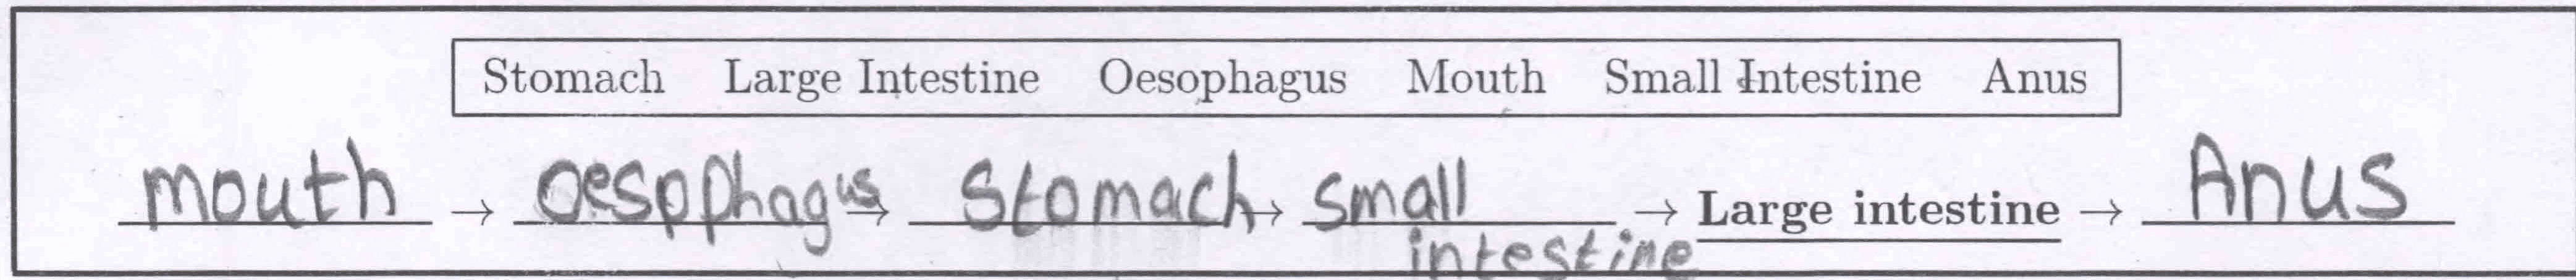
\includegraphics[width=5cm]{Q60_D117191_Science.png}}
    \end{minipage}
    \vspace{10pt}

  

    % Image: Q60_D117197_Science.png - Scaled height: 2.00mm
    \begin{minipage}{\linewidth}
    \RaggedRight\textbf{\tiny \highred{Dharshan K [C]}} \\ 
    \vspace{4.00pt}\fcolorbox{blue}{white}{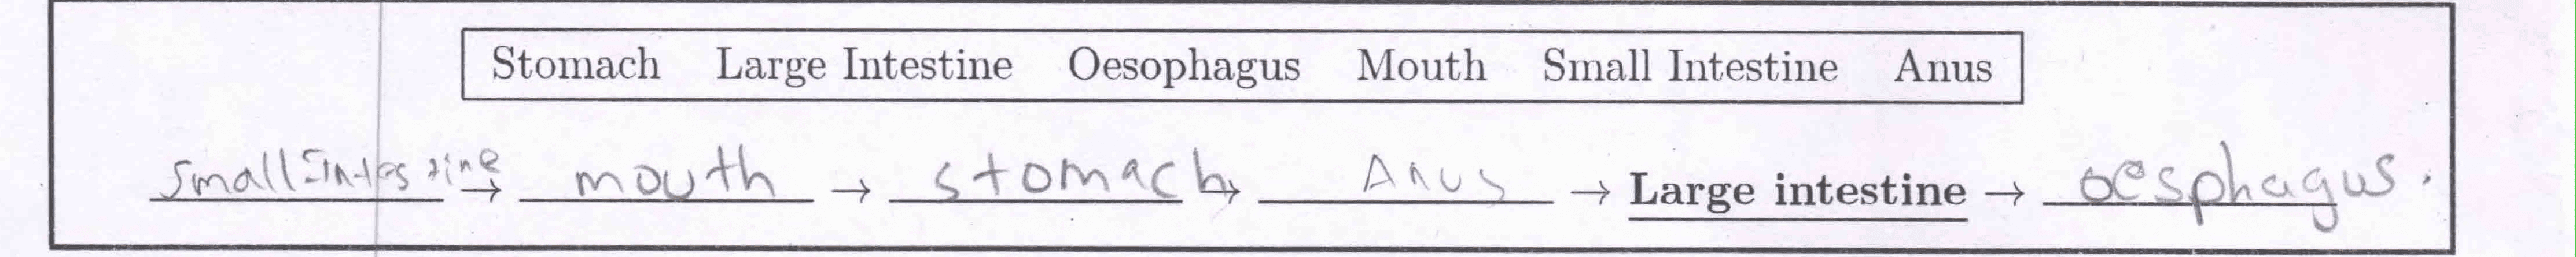
\includegraphics[width=5cm]{Q60_D117197_Science.png}}
    \end{minipage}
    \vspace{10pt}

    % Image: Q60_D117199_Science.png - Scaled height: 1.99mm
    \begin{minipage}{\linewidth}
    \RaggedRight\textbf{\tiny \highred{Karthick V [C]}} \\ 
    \vspace{4.00pt}\fcolorbox{blue}{white}{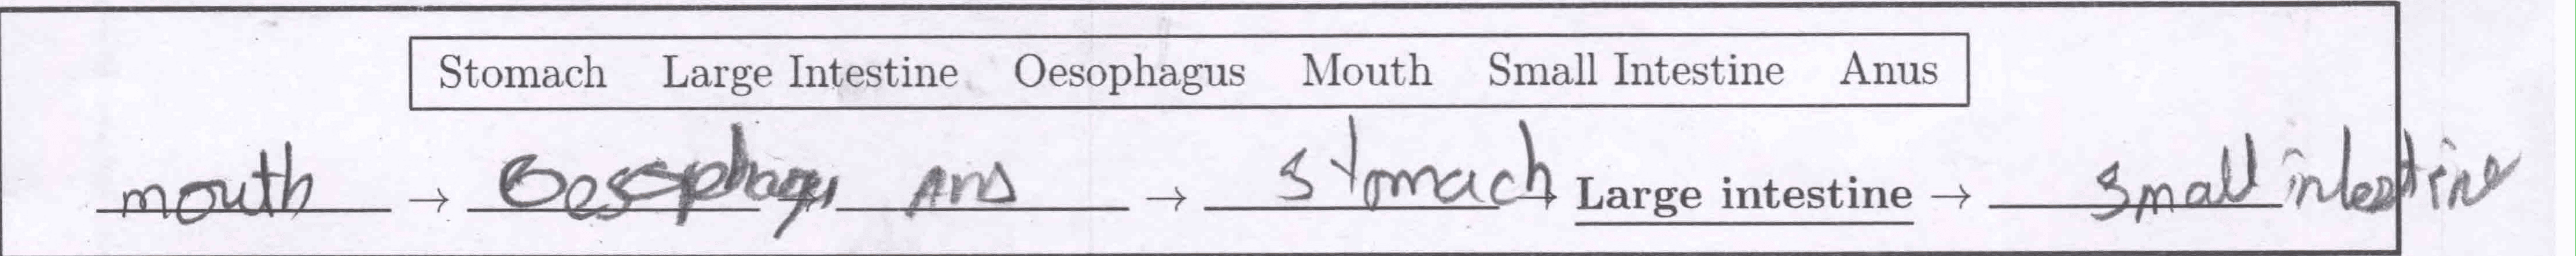
\includegraphics[width=5cm]{Q60_D117199_Science.png}}
    \end{minipage}
    \vspace{10pt}

    % Image: Q60_D117205_Science.png - Scaled height: 1.98mm
    \begin{minipage}{\linewidth}
    \RaggedRight\textbf{\tiny \highgreen{Divya Dharshini R J [D]}} \\ 
    \vspace{4.00pt}\fcolorbox{blue}{white}{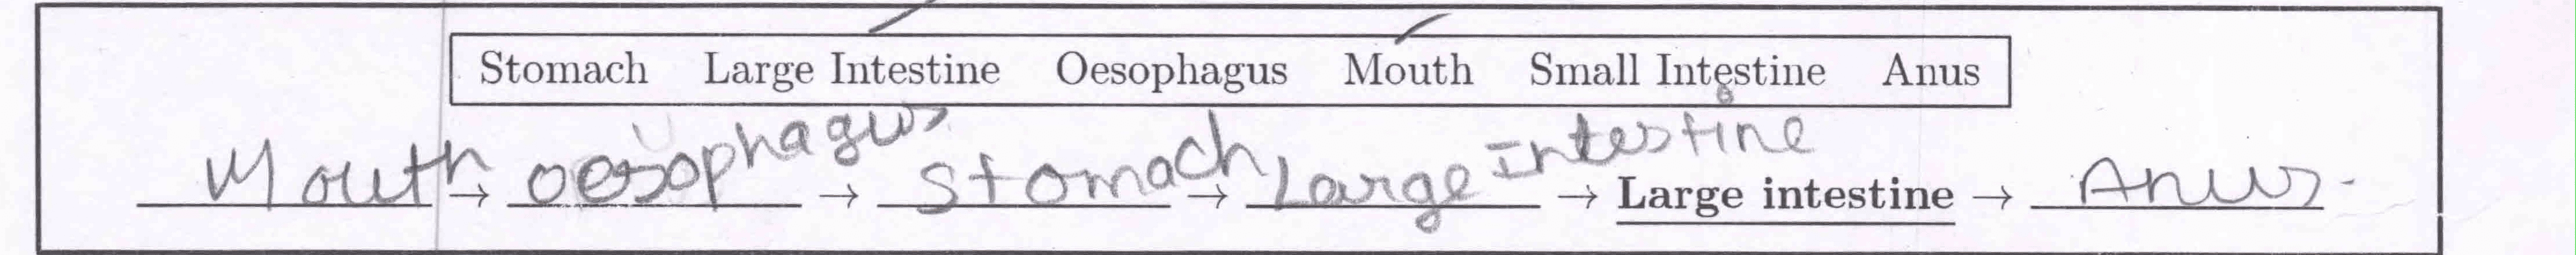
\includegraphics[width=5cm]{Q60_D117205_Science.png}}
    \end{minipage}
    \vspace{10pt}

    % Image: Q60_D117206_Science.png - Scaled height: 6.77mm
    \begin{minipage}{\linewidth}
    \RaggedRight\textbf{\tiny \highred{Hansika S R [C]}} \\ 
    \vspace{4.00pt}\fcolorbox{blue}{white}{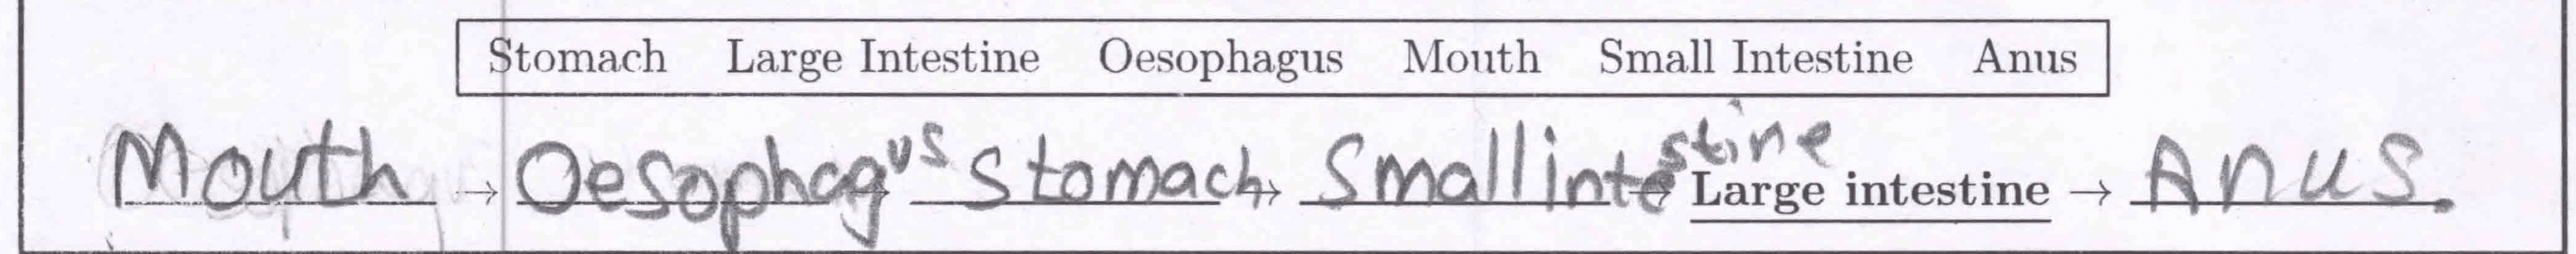
\includegraphics[width=5cm]{Q60_D117206_Science.png}}
    \end{minipage}
    \vspace{10pt}

    % Image: Q60_D117209_Science.png - Scaled height: 2.00mm
    \begin{minipage}{\linewidth}
    \RaggedRight\textbf{\tiny \highgreen{Mahaswetha S [D]}} \\ 
    \vspace{4.00pt}\fcolorbox{blue}{white}{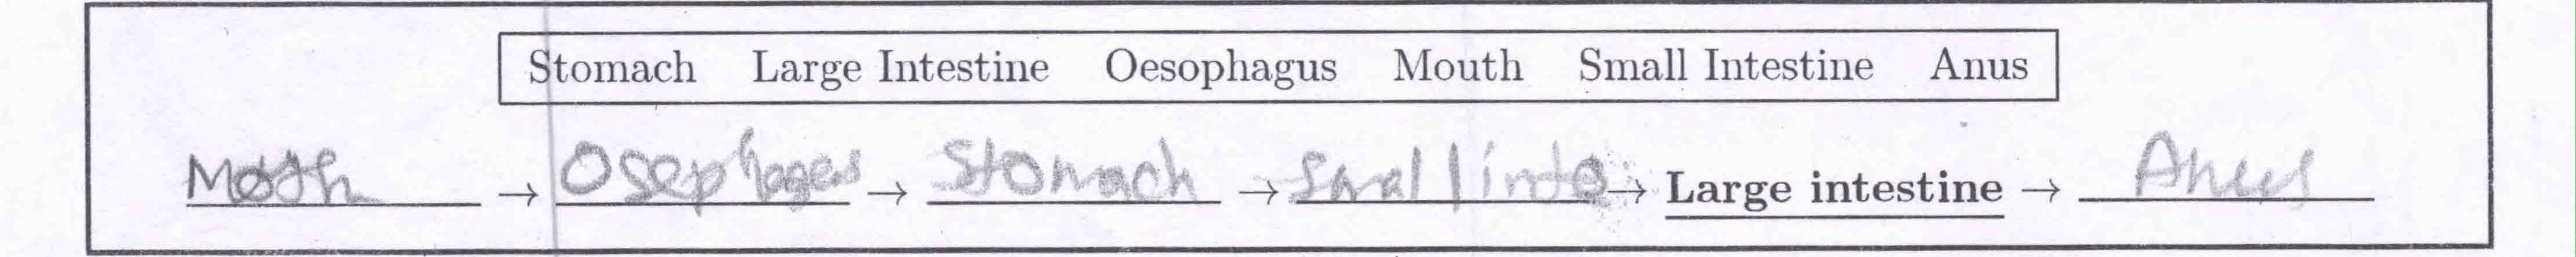
\includegraphics[width=5cm]{Q60_D117209_Science.png}}
    \end{minipage}
    \vspace{10pt}

    % Image: Q60_D117210_Science.png - Scaled height: 1.92mm
    \begin{minipage}{\linewidth}
    \RaggedRight\textbf{\tiny \highgreen{Swathi Sree K M [D]}} \\ 
    \vspace{4.00pt}\fcolorbox{blue}{white}{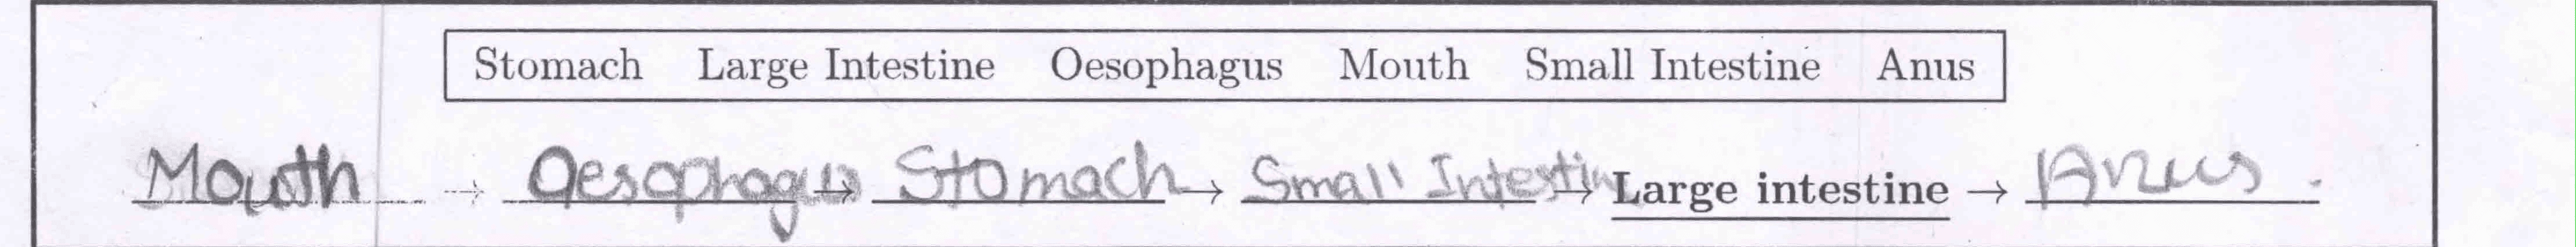
\includegraphics[width=5cm]{Q60_D117210_Science.png}}
    \end{minipage}
    \vspace{10pt}

    % Image: Q60_D117211_Science.png - Scaled height: 2.01mm
    \begin{minipage}{\linewidth}
    \RaggedRight\textbf{\tiny \highred{Tanu Shree R S [C]}} \\ 
    \vspace{4.00pt}\fcolorbox{blue}{white}{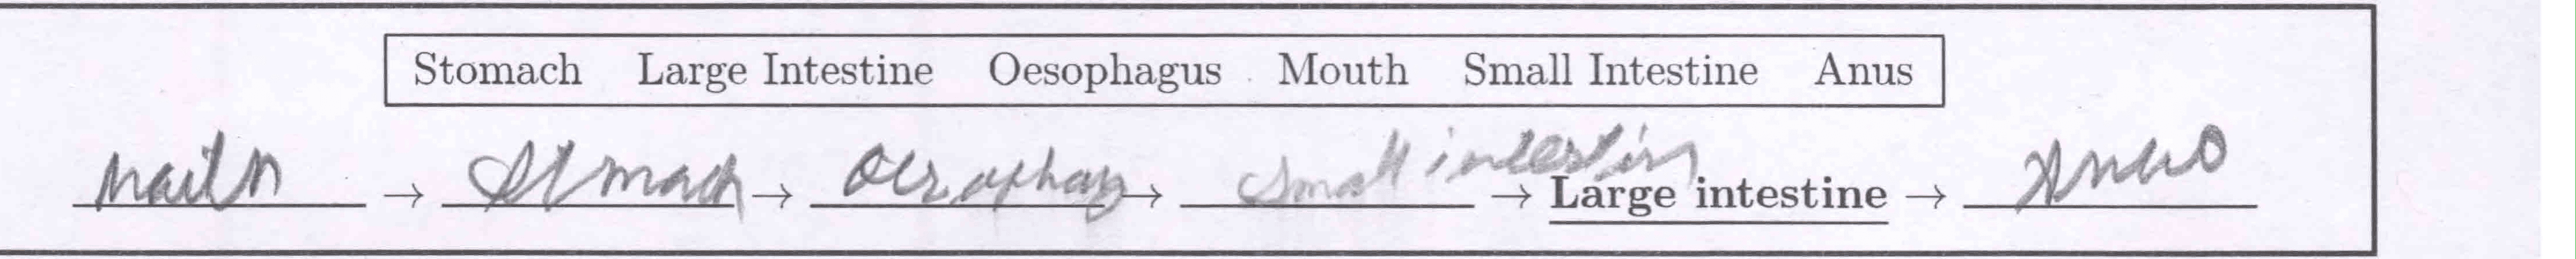
\includegraphics[width=5cm]{Q60_D117211_Science.png}}
    \end{minipage}
    \vspace{10pt}

    \end{multicols}
\end{frame}




\begin{frame}[shrink=0.1,label=QPC7QC7S04 - DT - Q1]{Q15 [3. Heat]}
\vspace{-0.2cm}
\mcqimgleftFourOne{
  questionnumber={15}, 
  questionTag={C7S04 – DT – Q1},
  questiontext={Identify the temperature in the given clinical thermometer.},
  imgtabletikz = { {\adjustbox{scale=\scalefactor}{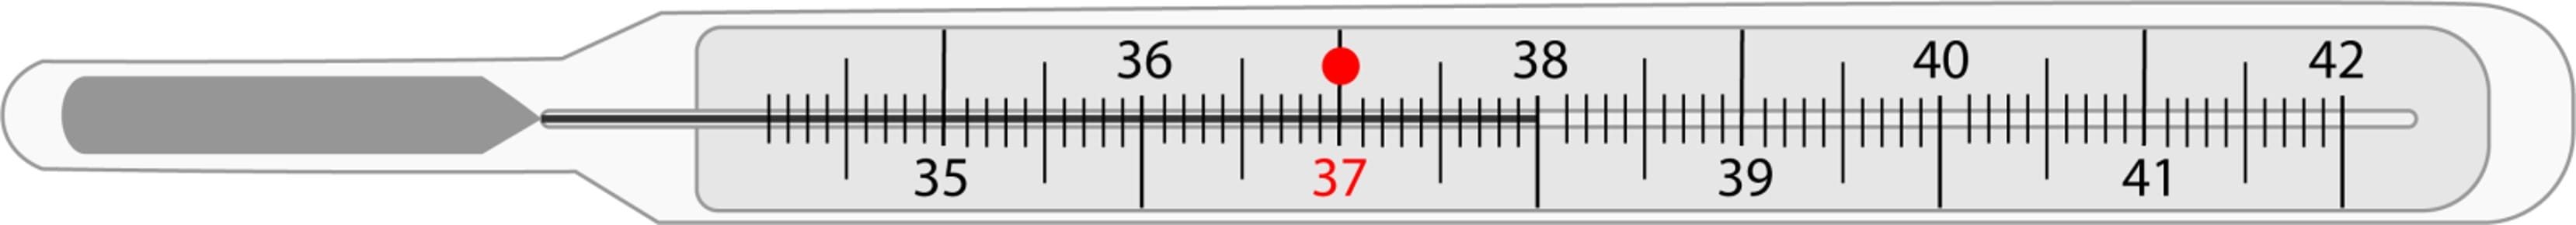
\includegraphics[width=15cm,height=1.5cm]{C7S04 – DT – Q1 .jpg}}} },
  optionA={37°C},
  optionB={36°C},
  optionC={38°C},
  optionD={42°C},
  correctoption={C},
  leftmini={0.8},
  rightmini={0.1},
}

\begin{minipage}{\linewidth}
\hspace{1cm}
\centering
\tiny
\renewcommand{\arraystretch}{1.25}
\begin{tabular}{|M{1.2cm}|M{0.8cm}|M{0.8cm}|M{0.8cm}|M{0.8cm}|M{0.8cm}|}
\hline
Option & A (\ding{55}) & B (\ding{55}) & \cellcolor{cellgreen} C (\ding{51}) & D (\ding{55}) & E \\ 
\hline
7 A & \highno{44\%} & \highno{6\%} & \highred{38\%} & \highno{13\%} & \highno{0\%} \\ 
 \hline 
7 B & \highno{29\%} & \highno{7\%} & \highno{64\%} & \highno{0\%} & \highno{0\%} \\ \hline
\end{tabular}
\end{minipage}

\end{frame}
% \input{4. PPT/6. My Answer/Science/C7/117_C7S - Q15}


\begin{frame}[shrink=0.1,label=QPC7QC7S04 - DT - Q10]{Q19 [3. Heat]}
\vspace{-0.2cm}
\mcqtextbottomTwoTwo{
  questionnumber={19}, 
  questionTag={C7S04 – DT – Q10}, 
  questiontext={Digital thermometer is used to measure the body temperature.\\Maximum-minimum thermometer helps us in giving the \rule{80pt}{0.1pt}.},
  optionA={Exact temperature of the object },
  optionB={Weather report},
  optionC={Rainfall},
  optionD={Pressure difference},
  correctoption={B},}

\begin{minipage}{\linewidth}
\hspace{1cm}
\centering
\tiny
\renewcommand{\arraystretch}{1.25}
\begin{tabular}{|M{1.2cm}|M{0.8cm}|M{0.8cm}|M{0.8cm}|M{0.8cm}|M{0.8cm}|}
\hline
Option & A (\ding{55}) & \cellcolor{cellgreen} B (\ding{51}) & C (\ding{55}) & D (\ding{55}) & E \\ 
\hline
7 A & \highno{44\%} & \highred{31\%} & \highno{0\%} & \highno{25\%} & \highno{0\%} \\ 
 \hline 
7 B & \highno{14\%} & \highno{57\%} & \highno{7\%} & \highno{21\%} & \highno{0\%} \\ \hline
\end{tabular}
\end{minipage}

\end{frame}
% \input{4. PPT/6. My Answer/Science/C7/117_C7S - Q19}


\begin{frame}[shrink=0.1,label=QPC7QC7S04 - DT - Q6]{Q25 [3. Heat]}
\vspace{-0.2cm}
\mcqtextbottomOneFour{
  questionnumber={25}, 
  questionTag={C7S04 – DT – Q6}, 
  questiontext={The heat from the sun is directly absorbed by our body through a process called  \rule{50pt}{0.1pt}.},
  optionA={Convection},
  optionB={Insulation},
  optionC={Reflection},
  optionD={Radiation},
  correctoption={D},
}

\begin{minipage}{\linewidth}
\hspace{1cm}
\centering
\tiny
\renewcommand{\arraystretch}{1.25}
\begin{tabular}{|M{1.2cm}|M{0.8cm}|M{0.8cm}|M{0.8cm}|M{0.8cm}|M{0.8cm}|}
\hline
Option & A (\ding{55}) & B (\ding{55}) & C (\ding{55}) & \cellcolor{cellgreen} D (\ding{51}) & E \\ 
\hline
7 A & \highno{0\%} & \highno{0\%} & \highno{0\%} & \highgreen{100\%} & \highno{0\%} \\ 
 \hline 
7 B & \highno{14\%} & \highno{0\%} & \highno{14\%} & \highno{71\%} & \highno{0\%} \\ \hline
\end{tabular}
\end{minipage}

\end{frame}
% \input{4. PPT/6. My Answer/Science/C7/117_C7S - Q25}


\begin{frame}[shrink=0.1,label=QPC7QC7S04 - DT - Q26]{Q27 [3. Heat]}
\vspace{-0.2cm}

\mcqtextbottomFourOne{
  questionnumber={27}, 
  questionTag={C7S04 – DT – Q26}, 
  questiontext={Why do you think kink is an important part in a clinical thermometer?},
  optionA={It helps in the free flow of mercury, so that the change in temperature can be noted.},
  optionB={It protects thermometer bulb from blast as the temperature increases. },
  optionC={It holds mercury level which helps to note the reading in the thermometer.},
  optionD={It acts as a cell and gives electrical energy to note the reading in the thermometer. },
  correctoption={C},
}

\begin{minipage}{\linewidth}
\hspace{1cm}
\centering
\tiny
\renewcommand{\arraystretch}{1.25}
\begin{tabular}{|M{1.2cm}|M{0.8cm}|M{0.8cm}|M{0.8cm}|M{0.8cm}|M{0.8cm}|}
\hline
Option & A (\ding{55}) & B (\ding{55}) & \cellcolor{cellgreen} C (\ding{51}) & D (\ding{55}) & E \\ 
\hline
7 A & \highno{25\%} & \highno{13\%} & \highno{50\%} & \highno{13\%} & \highno{0\%} \\ 
 \hline 
7 B & \highno{29\%} & \highno{21\%} & \highno{50\%} & \highno{0\%} & \highno{0\%} \\ \hline
\end{tabular}
\end{minipage}

\end{frame}
% \input{4. PPT/6. My Answer/Science/C7/117_C7S - Q27}


\begin{frame}[shrink=0.1,label=QPC7QC7S04 - DT - Q16]{Q33 [3. Heat]}
\vspace{-0.2cm}

\mcqtextbottomTwoTwo{
  questionnumber={33}, 
  questionTag={C7S04 – DT – Q16}, 
  questiontext={Which among the following is a necessary condition for heat transfer by conduction?},
  optionA={Objects should maintain zero temperature},
  optionB={Direct contact between objects},
  optionC={Objects should be made of metals},
  optionD={Medium of objects should be liquids},
  correctoption={B},
}

\begin{minipage}{\linewidth}
\hspace{1cm}
\centering
\tiny
\renewcommand{\arraystretch}{1.25}
\begin{tabular}{|M{1.2cm}|M{0.8cm}|M{0.8cm}|M{0.8cm}|M{0.8cm}|M{0.8cm}|}
\hline
Option & A (\ding{55}) & \cellcolor{cellgreen} B (\ding{51}) & C (\ding{55}) & D (\ding{55}) & E \\ 
\hline
7 A & \highno{13\%} & \highred{13\%} & \highno{25\%} & \highno{44\%} & \highno{6\%} \\ 
 \hline 
7 B & \highno{7\%} & \highred{29\%} & \highno{50\%} & \highno{14\%} & \highno{0\%} \\ \hline
\end{tabular}
\end{minipage}

\end{frame}
% \input{4. PPT/6. My Answer/Science/C7/117_C7S - Q33}


\begin{frame}[shrink=0.1,label=QPC7QC7S04 - DT - Q27]{Q54 [3. Heat]}
\vspace{-0.2cm}

\matextbottomOneFour{
myanswerquestion={Fill in the blanks based on materials conducting property},
myanswercontent={
\begin{enumerate}
    \item Materials that allow electricity and heat to pass through them easily are called \rule{100pt}{0.5pt}(Conductor/Insulator)
    \item Materials that do not allow heat and electricity to pass through them are called \rule{100pt}{0.5pt}(Conductor/Insulator)
\end{enumerate}
},
questionnumber={54}, 
questionTag={C7S04 - DT - Q27}, 
questiontext={Which material acts as a very good conductor of heat in cooking?},
optionA={
\tikzset{every picture/.style={line width=0.75pt,scale=\scalefactor}} 
\begin{tikzpicture}[x=0.75pt,y=0.75pt,yscale=-1,xscale=1]
\draw (91.5,99.3) node  {\adjustbox{scale=\scalefactor}{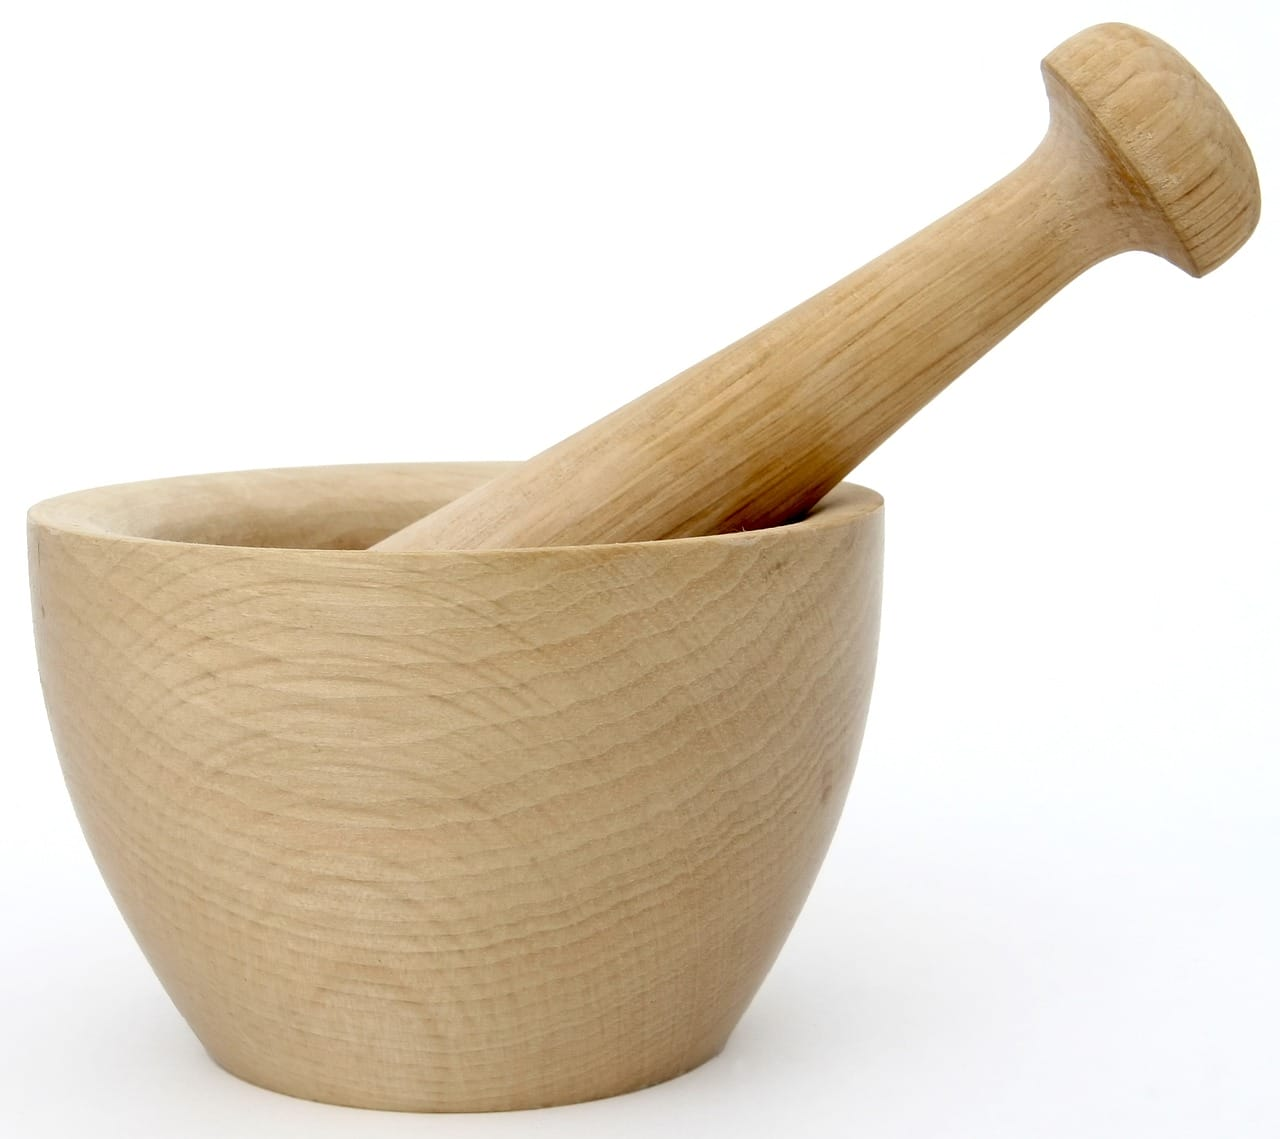
\includegraphics[width=50pt,height=50pt]{C7S04 – DT – Q13i.png}}};
\draw (46,150.2) node [anchor=north west][inner sep=0.75pt]   [align=left] {Wood crusher};
\end{tikzpicture}
},
optionB={
\tikzset{every picture/.style={line width=0.75pt,scale=\scalefactor}} 
\begin{tikzpicture}[x=0.75pt,y=0.75pt,yscale=-1,xscale=1]
\draw (84.5,96.3) node  {\adjustbox{scale=\scalefactor}{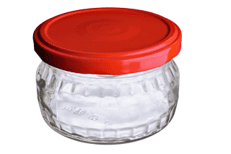
\includegraphics[width=50pt,height=50pt]{C7S04 – DT – Q13ii.png}}};
\draw (39,152) node [anchor=north west][inner sep=0.75pt]   [align=left] {Glass jar};
\end{tikzpicture}
},
optionC={
\tikzset{every picture/.style={line width=0.75pt,scale=\scalefactor}}     
\begin{tikzpicture}[x=0.75pt,y=0.75pt,yscale=-1,xscale=1]
\draw (87.2,160.3) node  {\adjustbox{scale=\scalefactor}{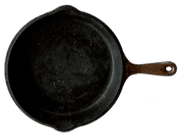
\includegraphics[width=50pt,height=50pt]{C7S04 – DT – Q13iii.png}}};
\draw (42,213) node [anchor=north west][inner sep=0.75pt]   [align=left] {Iron pan};
\end{tikzpicture}
},
optionD={
\tikzset{every picture/.style={line width=0.75pt,scale=\scalefactor}} 
\begin{tikzpicture}[x=0.75pt,y=0.75pt,yscale=-1,xscale=1]
\draw (78.2,108.8) node  {\adjustbox{scale=\scalefactor}{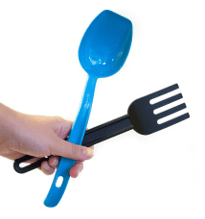
\includegraphics[width=50pt,height=50pt]{C7S04 – DT – Q13iv.png}}};
\draw (34,162) node [anchor=north west][inner sep=0.75pt]   [align=left] {Plastic spoons};
\end{tikzpicture}
},
correctoption={C},
}




\begin{minipage}{\linewidth}
\hspace{1cm}
\centering
\tiny
\renewcommand{\arraystretch}{1.25}
\begin{tabular}{|M{1.2cm}|M{0.8cm}|M{0.8cm}|M{0.8cm}|M{0.8cm}|M{0.8cm}|}
\hline
Option & A (\ding{55}) & B (\ding{55}) & \cellcolor{cellgreen} C (\ding{51}) & D (\ding{55}) & E \\ 
\hline
7 A & \highno{0\%} & \highno{6\%} & \highgreen{88\%} & \highno{0\%} & \highno{6\%} \\ 
 \hline 
7 B & \highno{7\%} & \highno{0\%} & \highgreen{93\%} & \highno{0\%} & \highno{0\%} \\ \hline
\end{tabular}
\end{minipage}

\end{frame}
\begin{frame}{Q54 - My Answer Responses}
    \vspace{-0.6cm}
    \begin{multicols}{3}

    % Image: Q54_D117179_Science.png - Scaled height: 2.37mm
    \begin{minipage}{\linewidth}
    \RaggedRight\textbf{\tiny \highgreen{Kallis K [C]}} \\ 
    \vspace{4.00pt}\fcolorbox{blue}{white}{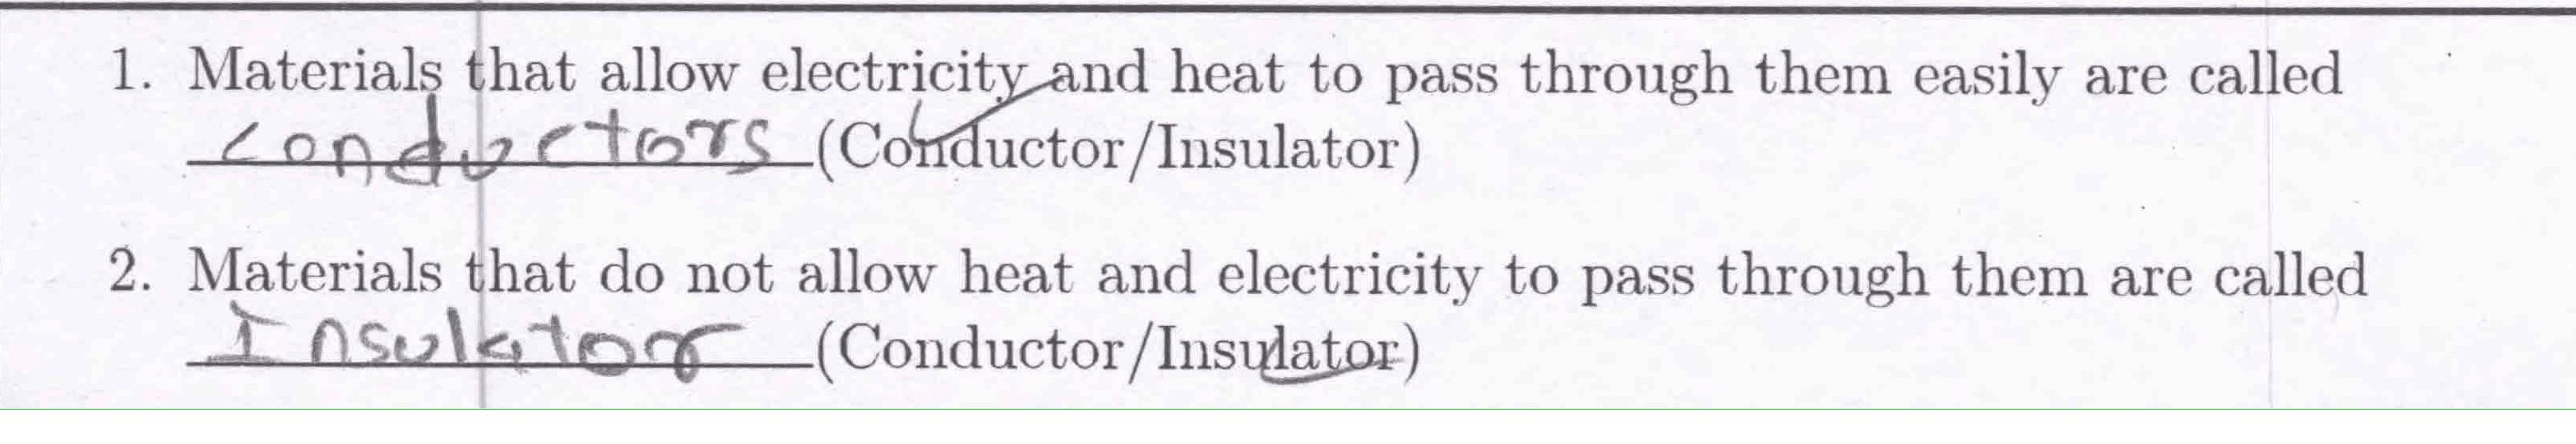
\includegraphics[width=4cm]{Q54_D117179_Science.png}}
    \end{minipage}
    \vspace{10pt}

    % Image: Q54_D117183_Science.png - Scaled height: 2.32mm
    \begin{minipage}{\linewidth}
    \RaggedRight\textbf{\tiny \highred{Srishravan N M [E]}} \\ 
    \vspace{4.00pt}\fcolorbox{blue}{white}{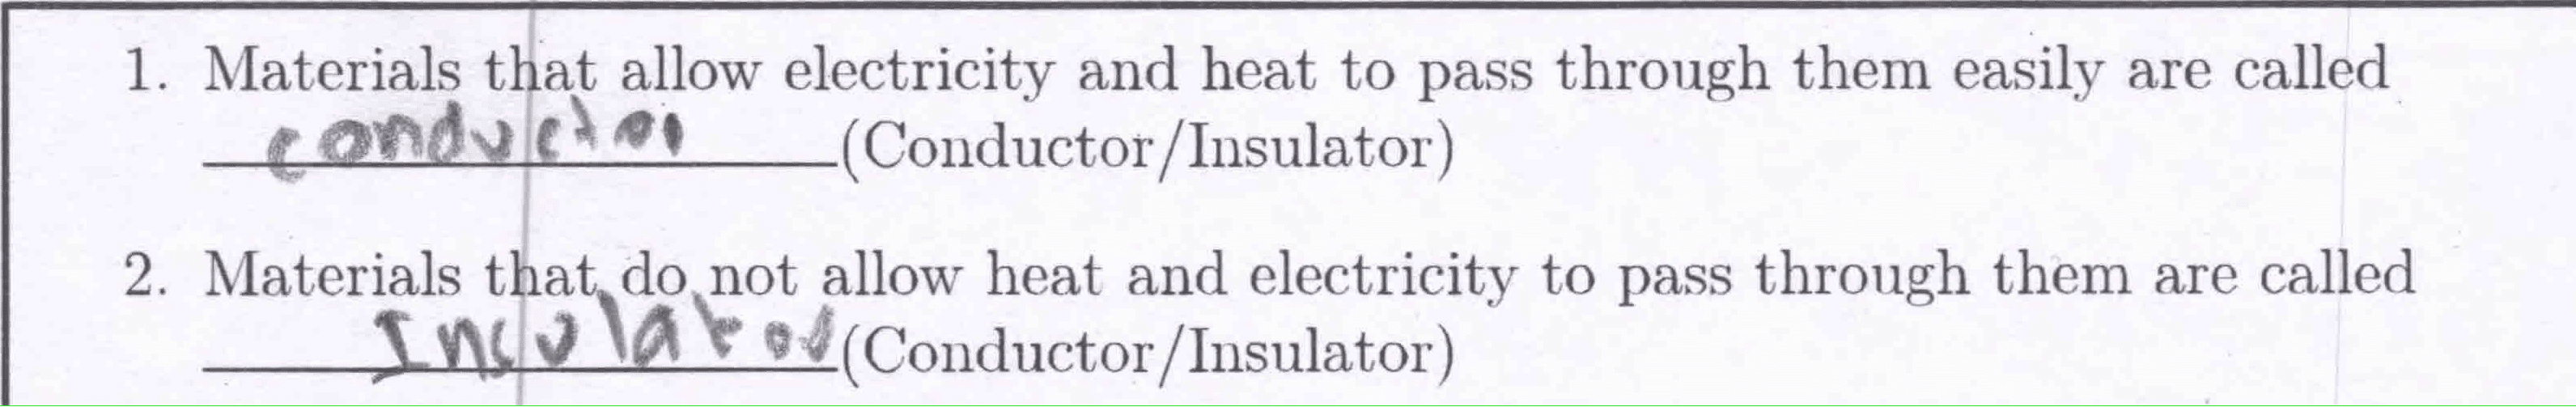
\includegraphics[width=4cm]{Q54_D117183_Science.png}}
    \end{minipage}
    \vspace{10pt}

    % Image: Q54_D117190_Science.png - Scaled height: 2.26mm
    \begin{minipage}{\linewidth}
    \RaggedRight\textbf{\tiny \highgreen{Mithra J R [C]}} \\ 
    \vspace{4.00pt}\fcolorbox{blue}{white}{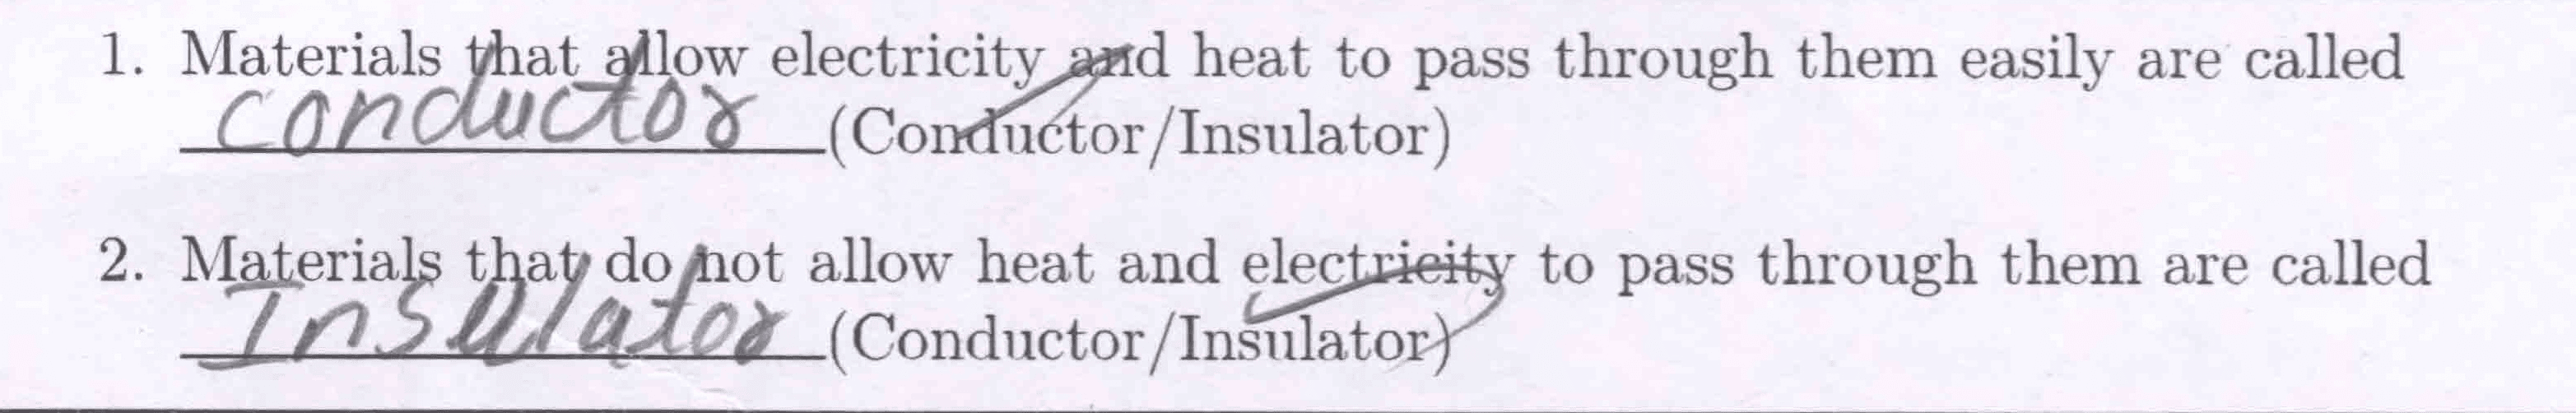
\includegraphics[width=4cm]{Q54_D117190_Science.png}}
    \end{minipage}
    \vspace{10pt}

    % Image: Q54_D117191_Science.png - Scaled height: 2.41mm
    \begin{minipage}{\linewidth}
    \RaggedRight\textbf{\tiny \highgreen{Sharlin Maria T [C]}} \\ 
    \vspace{4.00pt}\fcolorbox{blue}{white}{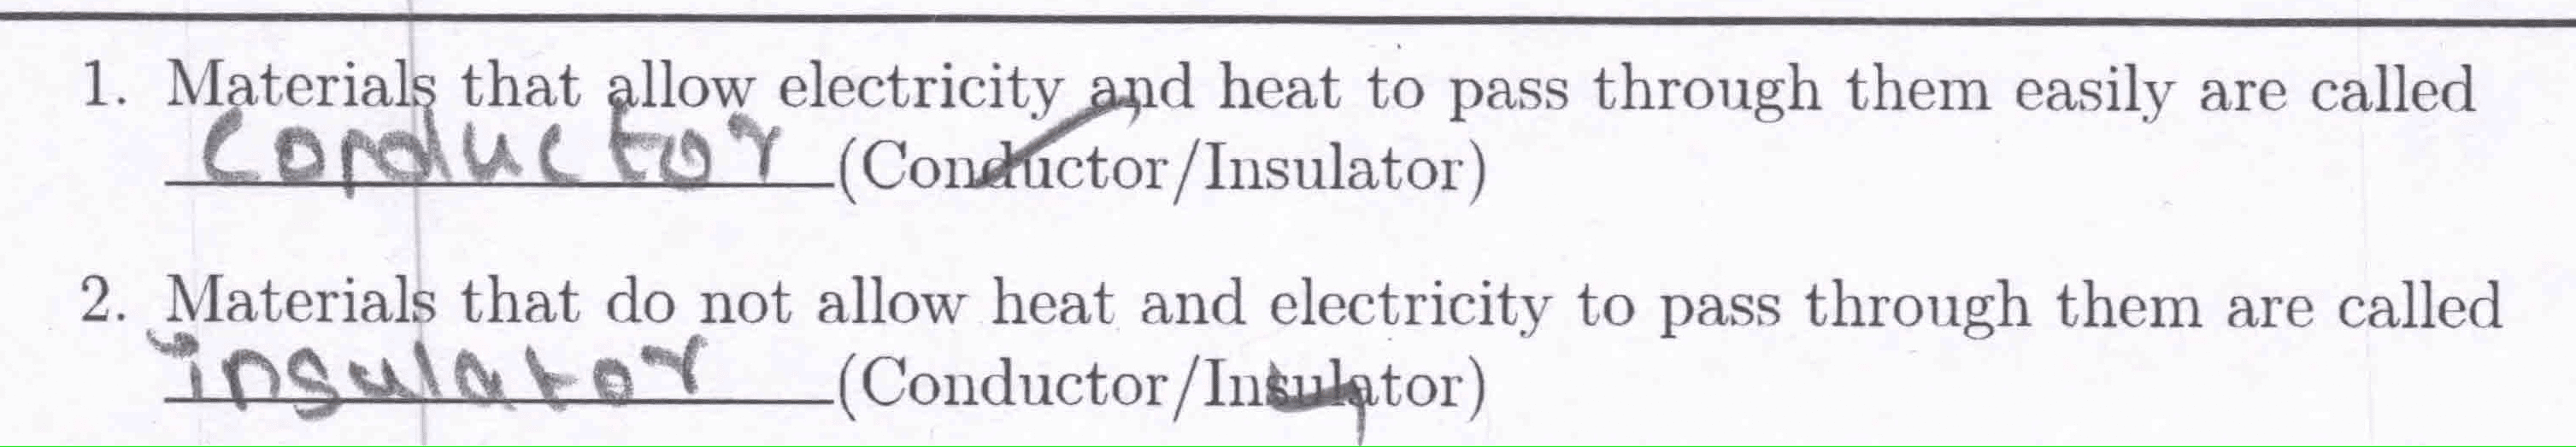
\includegraphics[width=4cm]{Q54_D117191_Science.png}}
    \end{minipage}
    \vspace{10pt}

    % Image: Q54_D117193_Science.png - Scaled height: 2.38mm
    \begin{minipage}{\linewidth}
    \RaggedRight\textbf{\tiny \highgreen{Siva Rubini R [C]}} \\ 
    \vspace{4.00pt}\fcolorbox{blue}{white}{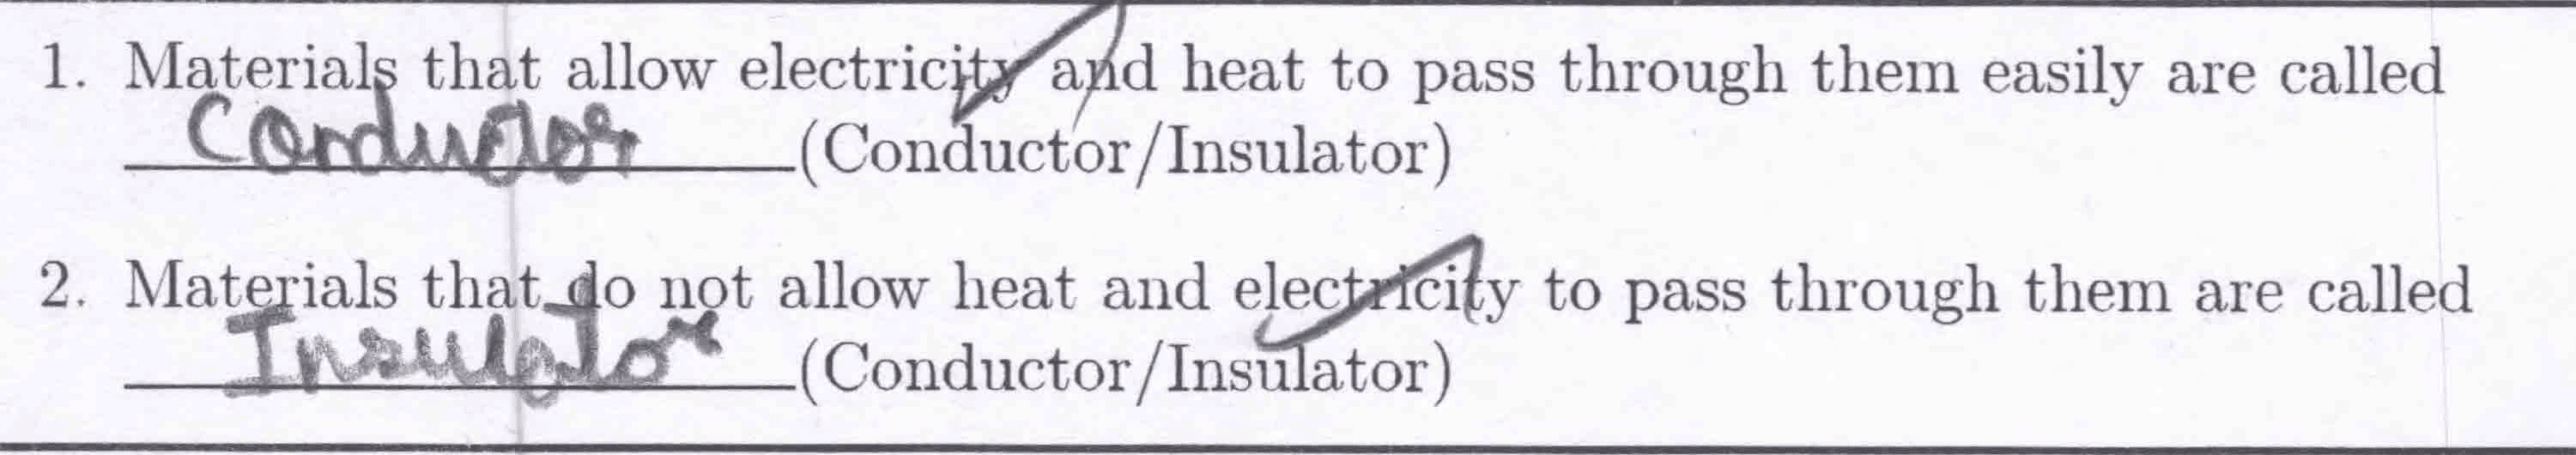
\includegraphics[width=4cm]{Q54_D117193_Science.png}}
    \end{minipage}
    \vspace{10pt}

    % Image: Q54_D117194_Science.png - Scaled height: 2.35mm
    \begin{minipage}{\linewidth}
    \RaggedRight\textbf{\tiny \highgreen{Tharsika S [C]}} \\ 
    \vspace{4.00pt}\fcolorbox{blue}{white}{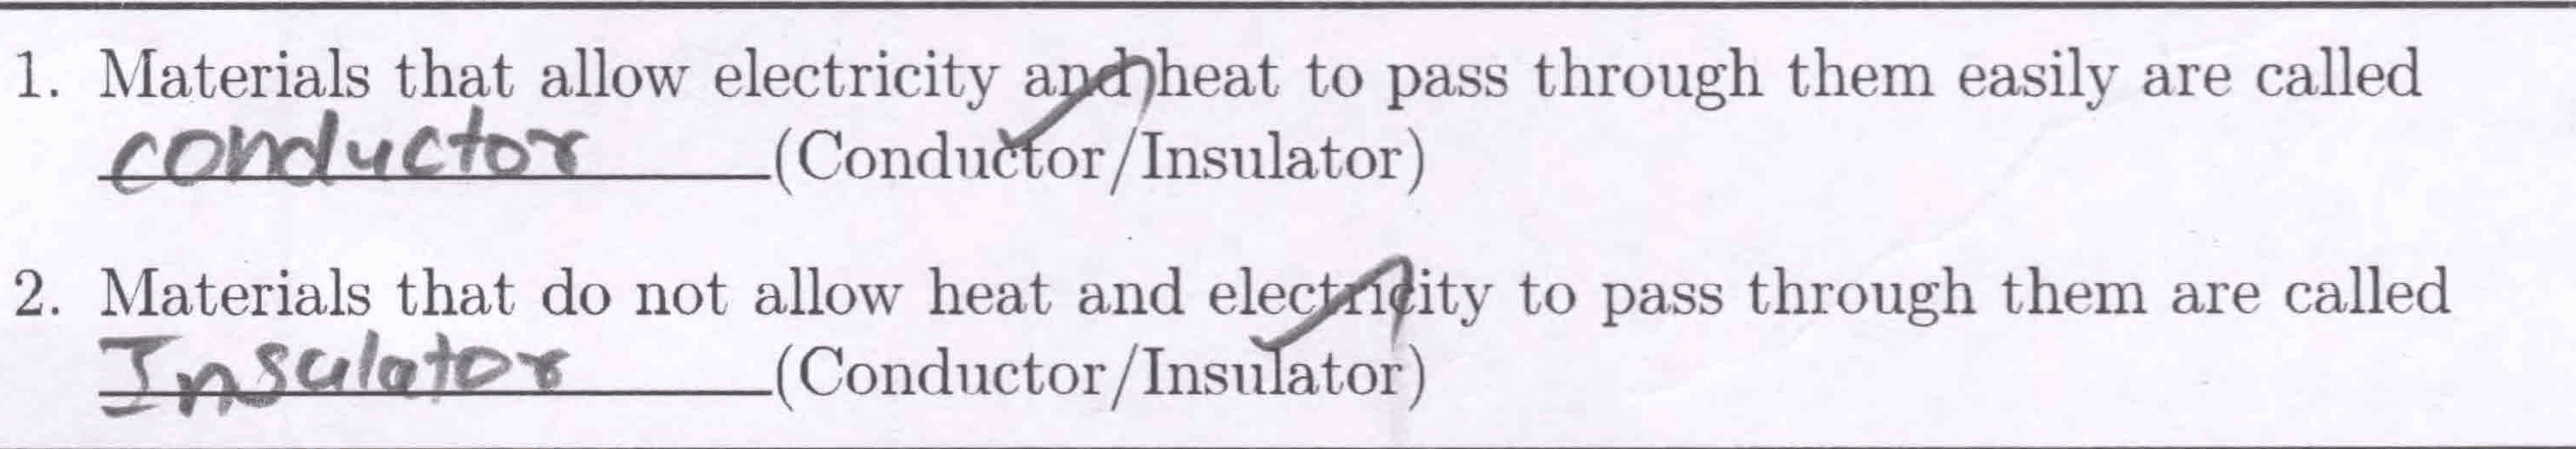
\includegraphics[width=4cm]{Q54_D117194_Science.png}}
    \end{minipage}
    \vspace{10pt}

    % Image: Q54_D117199_Science.png - Scaled height: 2.27mm
    \begin{minipage}{\linewidth}
    \RaggedRight\textbf{\tiny \highgreen{Karthick V [C]}} \\ 
    \vspace{4.00pt}\fcolorbox{blue}{white}{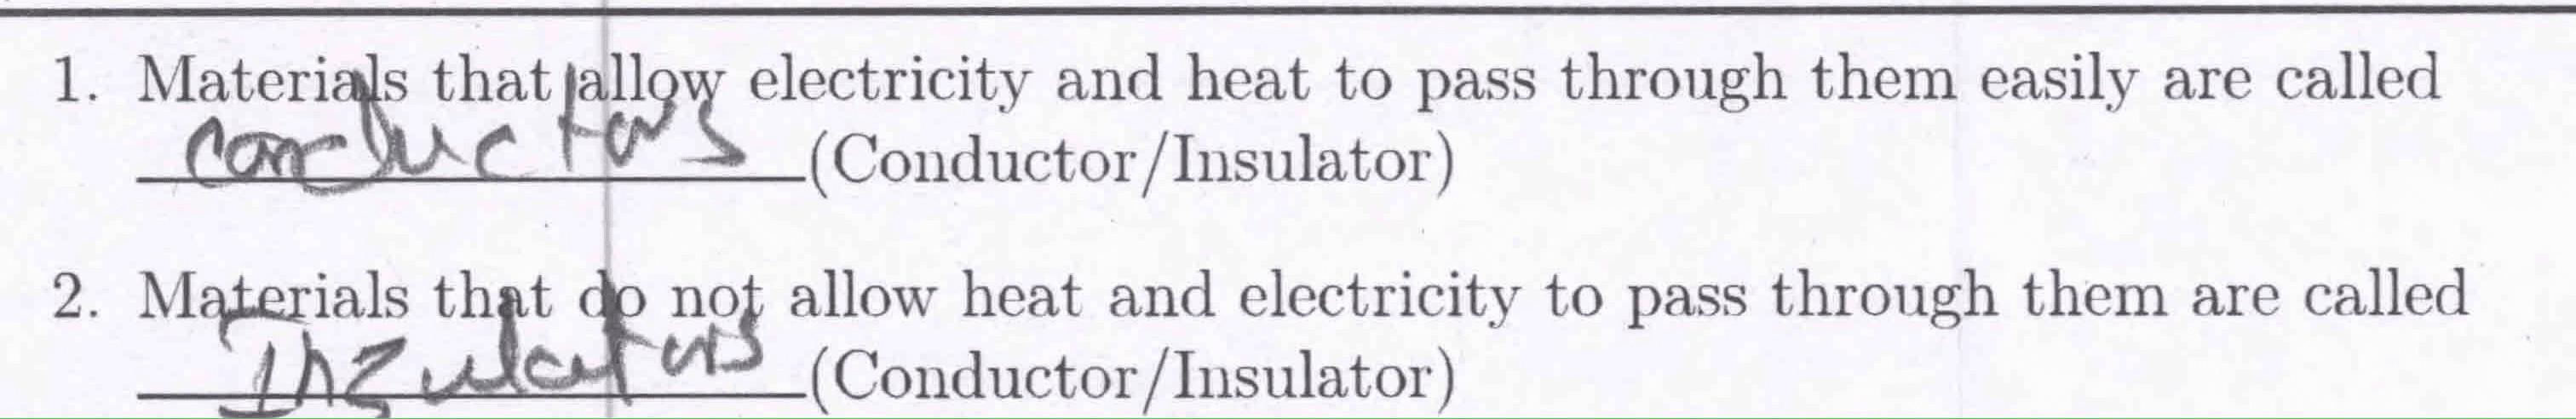
\includegraphics[width=4cm]{Q54_D117199_Science.png}}
    \end{minipage}
    \vspace{10pt}

    % Image: Q54_D117206_Science.png - Scaled height: 2.39mm
    \begin{minipage}{\linewidth}
    \RaggedRight\textbf{\tiny \highgreen{Hansika S R [C]}} \\ 
    \vspace{4.00pt}\fcolorbox{blue}{white}{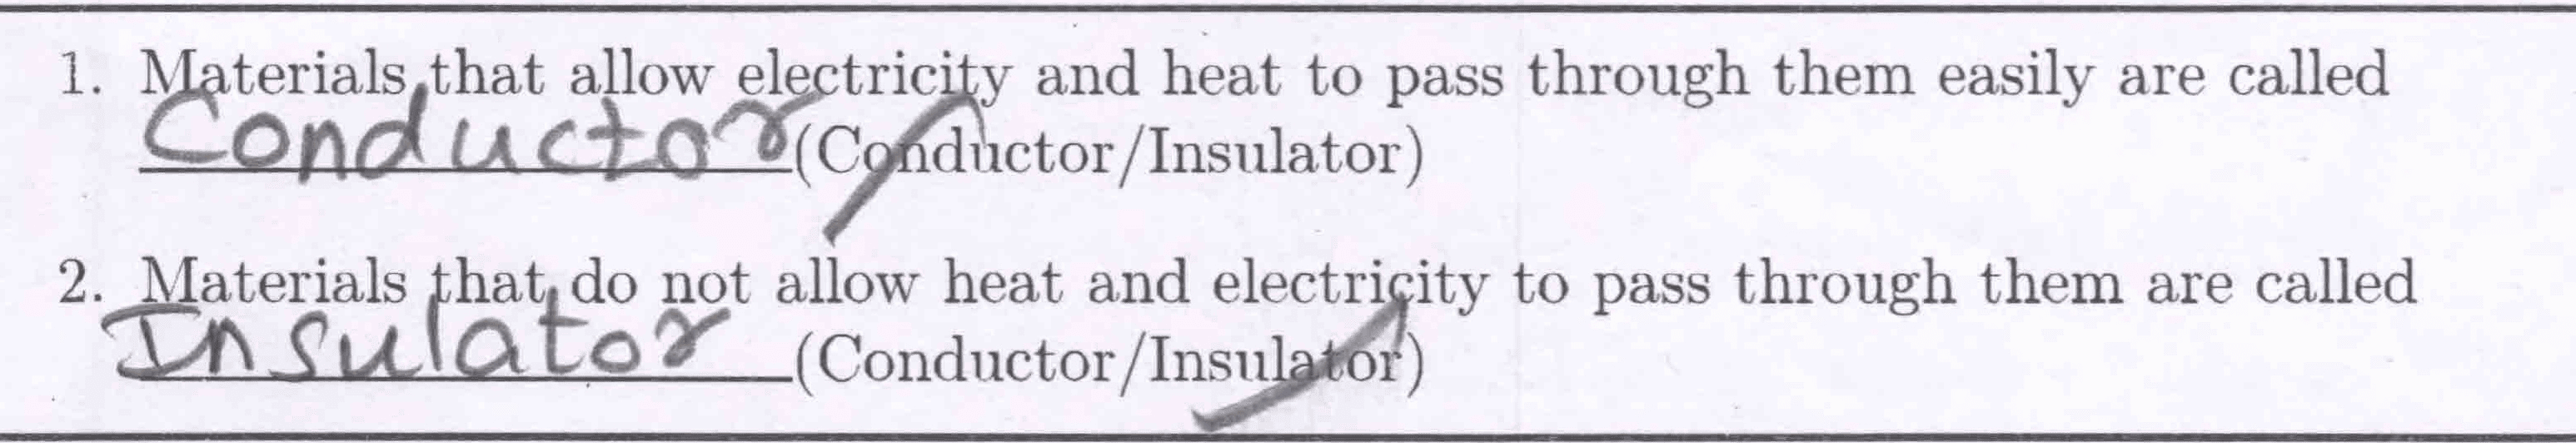
\includegraphics[width=4cm]{Q54_D117206_Science.png}}
    \end{minipage}
    \vspace{10pt}

    % Image: Q54_D117208_Science.png - Scaled height: 2.44mm
    \begin{minipage}{\linewidth}
    \RaggedRight\textbf{\tiny \highgreen{Karnika S E A [C]}} \\ 
    \vspace{4.00pt}\fcolorbox{blue}{white}{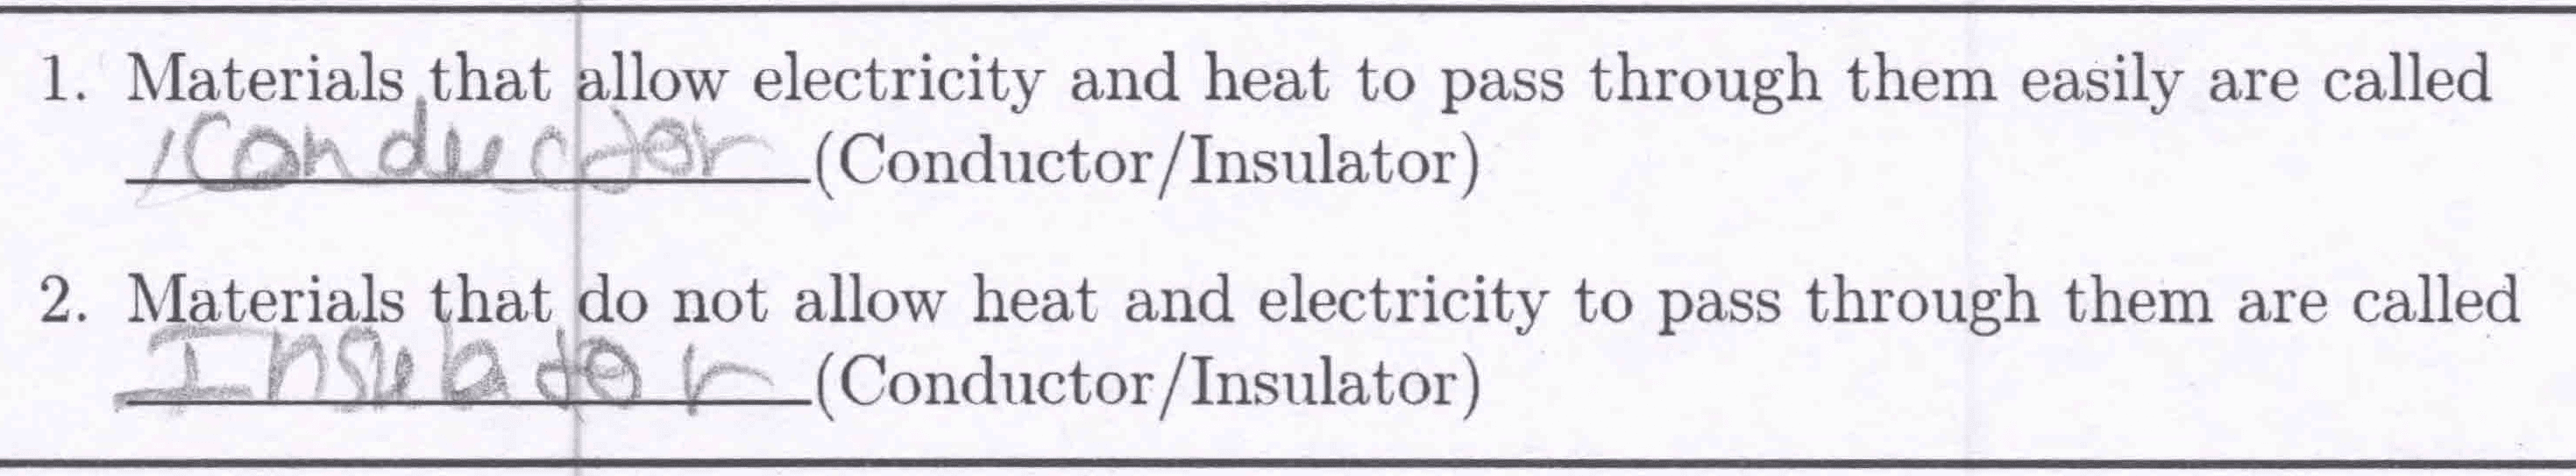
\includegraphics[width=4cm]{Q54_D117208_Science.png}}
    \end{minipage}
    \vspace{10pt}

    % Image: Q54_D117209_Science.png - Scaled height: 2.41mm
    \begin{minipage}{\linewidth}
    \RaggedRight\textbf{\tiny \highgreen{Mahaswetha S [C]}} \\ 
    \vspace{4.00pt}\fcolorbox{blue}{white}{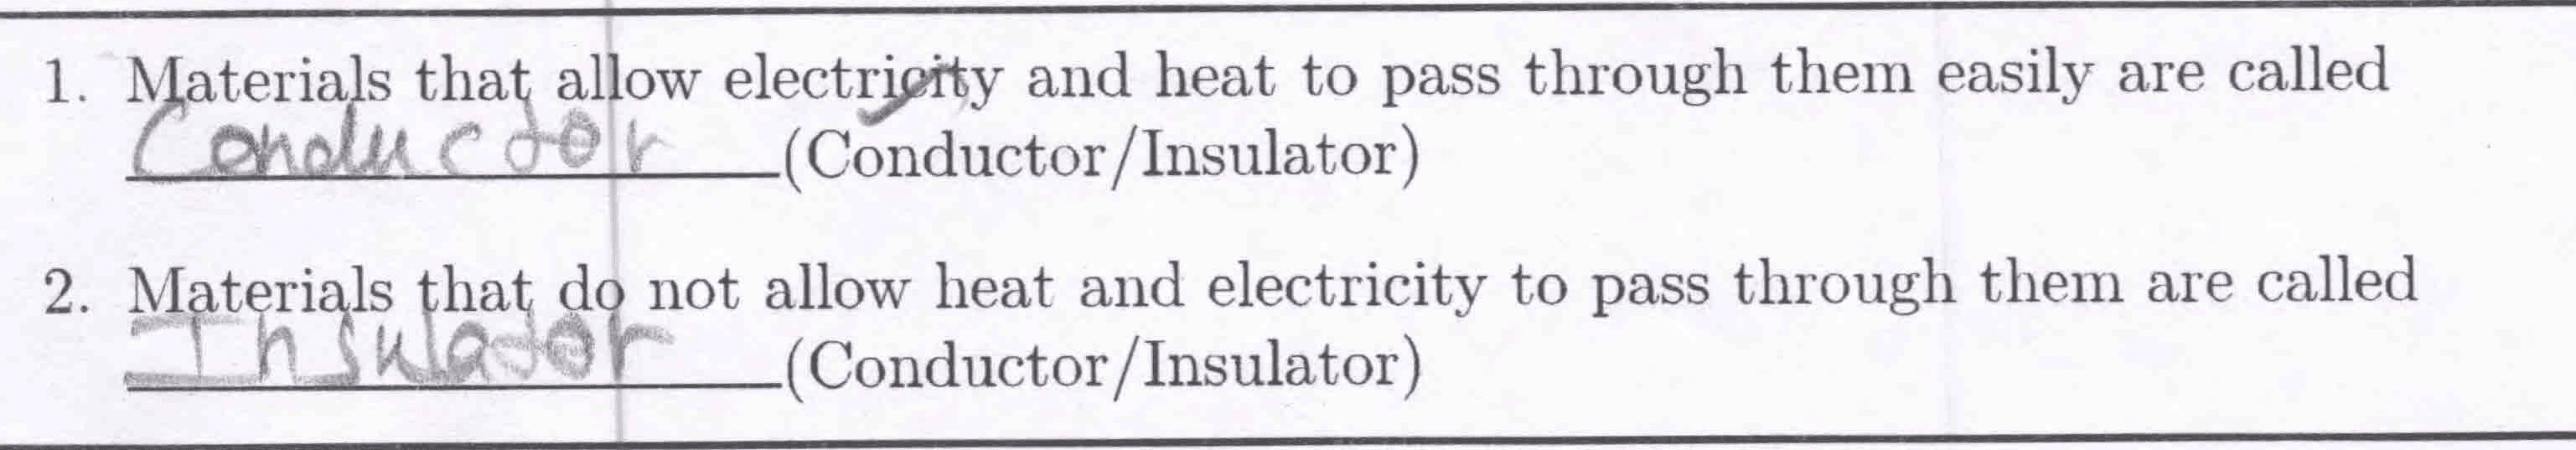
\includegraphics[width=4cm]{Q54_D117209_Science.png}}
    \end{minipage}
    \vspace{10pt}

    \end{multicols}
\end{frame}




\begin{frame}[shrink=0.1,label=QPC7QC7S05 - DT - Q8]{Q7 [4. Acids, Bases and Salts]}
\vspace{-0.2cm}
\mcqtextbottomTwoTwo{
  questionnumber={7}, 
  questionTag={C7S05 – DT – Q8}, 
  questiontext={Complete the neutralisation reaction.\\Hydrochloric acid (HCl) $+$ Sodium hydroxide (NaOH) $\rightarrow$ \rule{80pt}{0.1pt} $+$ Water (H$_2$O).},
  optionA={Hydrogen hydroxide (HOH)    },
  optionB={Sodium acid (NaOH)},
  optionC={Sodium chloride (NaCl)},
  optionD={Hydrogen chloride (HCl)},
  correctoption={C},
}

\begin{minipage}{\linewidth}
\hspace{1cm}
\centering
\tiny
\renewcommand{\arraystretch}{1.25}
\begin{tabular}{|M{1.2cm}|M{0.8cm}|M{0.8cm}|M{0.8cm}|M{0.8cm}|M{0.8cm}|}
\hline
Option & A (\ding{55}) & B (\ding{55}) & \cellcolor{cellgreen} C (\ding{51}) & D (\ding{55}) & E \\ 
\hline
7 A & \highno{0\%} & \highno{19\%} & \highno{69\%} & \highno{6\%} & \highno{6\%} \\ 
 \hline 
7 B & \highno{7\%} & \highno{29\%} & \highred{21\%} & \highno{43\%} & \highno{0\%} \\ \hline
\end{tabular}
\end{minipage}

\end{frame}
% \input{4. PPT/6. My Answer/Science/C7/117_C7S - Q7}


\begin{frame}[shrink=0.1,label=QPC7QC7S05 - DT - Q3]{Q23 [4. Acids, Bases and Salts]}
\vspace{-0.2cm}
\mcqtextbottomFourOne{
  questionnumber={23}, 
  questionTag={C7S05 – DT – Q3},
  questiontext={In chemistry, which of the following describes the role of indicators?},
  optionA={Indicators are tools used for measuring temperature.},
  optionB={Indicators are used to measure the volume of a liquid.},
  optionC={Indicators identify whether a solution is acidic, basic or neutral.},
  optionD={Indicators are used to change the colour of the solution.}, 
  correctoption={C},
}

\begin{minipage}{\linewidth}
\hspace{1cm}
\centering
\tiny
\renewcommand{\arraystretch}{1.25}
\begin{tabular}{|M{1.2cm}|M{0.8cm}|M{0.8cm}|M{0.8cm}|M{0.8cm}|M{0.8cm}|}
\hline
Option & A (\ding{55}) & B (\ding{55}) & \cellcolor{cellgreen} C (\ding{51}) & D (\ding{55}) & E \\ 
\hline
7 A & \highno{0\%} & \highno{6\%} & \highgreen{88\%} & \highno{6\%} & \highno{0\%} \\ 
 \hline 
7 B & \highno{0\%} & \highno{7\%} & \highgreen{79\%} & \highno{14\%} & \highno{0\%} \\ \hline
\end{tabular}
\end{minipage}

\end{frame}
% \input{4. PPT/6. My Answer/Science/C7/117_C7S - Q23}


\begin{frame}[shrink=0.1,label=QPC7QC7S05 - DT - Q2]{Q43 [4. Acids, Bases and Salts]}
\vspace{-0.2cm}
\mcqimgleftFourOne{
  questionnumber={43}, 
  questionTag={C7S05 – DT – Q2},
  questiontext={Match the following based on the nature of substances. },
  imgtabletikz= {\renewcommand{\arraystretch}{1.25}
\begin{tabular}{|p{0.25cm}|p{2cm}|p{0.25cm}|p{0.25cm}|p{2cm}|}
\hline
\multicolumn{2}{|c|}{Column A} & & \multicolumn{2}{|c|}{Column B} \\
\cline{1-2}\cline{4-5}
 i & Acid & & a& Phenolphthalein \\
\cline{1-2}\cline{4-5}
ii & Base  & & b & Lemon \\
\cline{1-2}\cline{4-5}
iii & Neutral & & c& Baking soda \\
\cline{1-2}\cline{4-5}
iv & Indicator & & d& Water \\
\hline
\end{tabular}},
  optionA={i–c, ii–d, iii–a, iv–b },
  optionB={i–b, ii–c, iii–d, iv–a },
  optionC={i–b, ii–d, iii–c, iv–a },
  optionD={i–d, ii–c, iii–b, iv–a },
  correctoption={B},
  leftmini={0.5},
  rightmini={0.4},
}

\begin{minipage}{\linewidth}
\hspace{1cm}
\centering
\tiny
\renewcommand{\arraystretch}{1.25}
\begin{tabular}{|M{1.2cm}|M{0.8cm}|M{0.8cm}|M{0.8cm}|M{0.8cm}|M{0.8cm}|}
\hline
Option & A (\ding{55}) & \cellcolor{cellgreen} B (\ding{51}) & C (\ding{55}) & D (\ding{55}) & E \\ 
\hline
7 A & \highno{13\%} & \highgreen{88\%} & \highno{0\%} & \highno{0\%} & \highno{0\%} \\ 
 \hline 
7 B & \highno{14\%} & \highgreen{79\%} & \highno{0\%} & \highno{7\%} & \highno{0\%} \\ \hline
\end{tabular}
\end{minipage}

\end{frame}
% \input{4. PPT/6. My Answer/Science/C7/117_C7S - Q43}


\begin{frame}[shrink=0.1,label=QPC7QC7S05 - DT - Q12]{Q52 [4. Acids, Bases and Salts]}
\vspace{-0.2cm}

\matextbottomTwoTwo{
myanswerquestion={Complete the following question based on the test on artificial indicators.},
myanswercontent={\begin{enumerate}
    \item Phenolphthalein is an \rule{80pt}{0.5pt}(natural/artificial) indicator used to test whether a solution is acidic or basic.
    \item The original colour of the phenolphthalein indicator is \rule{80pt}{0.5pt}.
    \item In acidic solutions, the colour of phenolphthalein is \rule{80pt}{0.5pt}.
    \item In basic solutions, the colour of phenolphthalein is \rule{80pt}{0.5pt}. 
\end{enumerate}},
questionnumber={52}, 
questionTag={C7S05 - DT - Q12}, 
questiontext={Find the colour change that takes place as a result of the reaction of the phenolphthalein indicator with acidic and basic solutions, respectively.},
optionA={Acid: Colourless, Base: Green},
optionB={Acid: Green, Base: Pink},
optionC={Acid: Colourless, Base: Pink},
optionD={Acid: Pink, Base: Colourless},
correctoption={C}
}




\begin{minipage}{\linewidth}
\hspace{1cm}
\centering
\tiny
\renewcommand{\arraystretch}{1.25}
\begin{tabular}{|M{1.2cm}|M{0.8cm}|M{0.8cm}|M{0.8cm}|M{0.8cm}|M{0.8cm}|}
\hline
Option & A (\ding{55}) & B (\ding{55}) & \cellcolor{cellgreen} C (\ding{51}) & D (\ding{55}) & E \\ 
\hline
7 A & \highno{25\%} & \highno{13\%} & \highred{25\%} & \highno{19\%} & \highno{19\%} \\ 
 \hline 
7 B & \highno{0\%} & \highno{43\%} & \highred{36\%} & \highno{21\%} & \highno{0\%} \\ \hline
\end{tabular}
\end{minipage}

\end{frame}
\begin{frame}{Q52 - My Answer Responses}
    \vspace{-0.6cm}
    \begin{multicols}{3}

    % Image: Q52_D117185_Science.png - Scaled height: 3.47mm
    \begin{minipage}{\linewidth}
    \RaggedRight\textbf{\tiny \highgreen{Sujay Kumar N [C]}} \\ 
    \vspace{4.00pt}\fcolorbox{blue}{white}{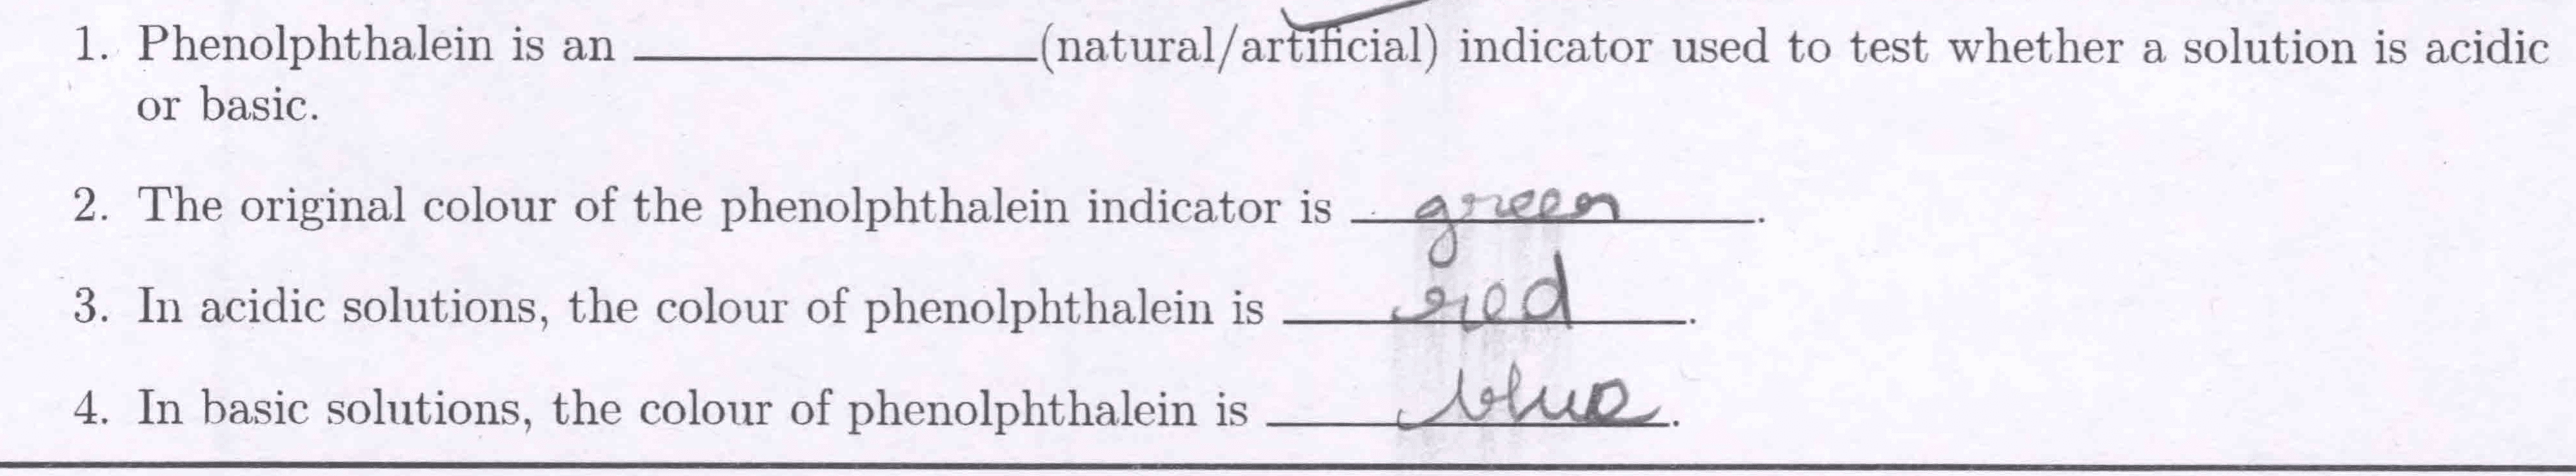
\includegraphics[width=4cm]{Q52_D117185_Science.png}}
    \end{minipage}
    \vspace{10pt}

    % Image: Q52_D117186_Science.png - Scaled height: 3.35mm
    \begin{minipage}{\linewidth}
    \RaggedRight\textbf{\tiny \highred{Yashwanth M [A]}} \\ 
    \vspace{4.00pt}\fcolorbox{blue}{white}{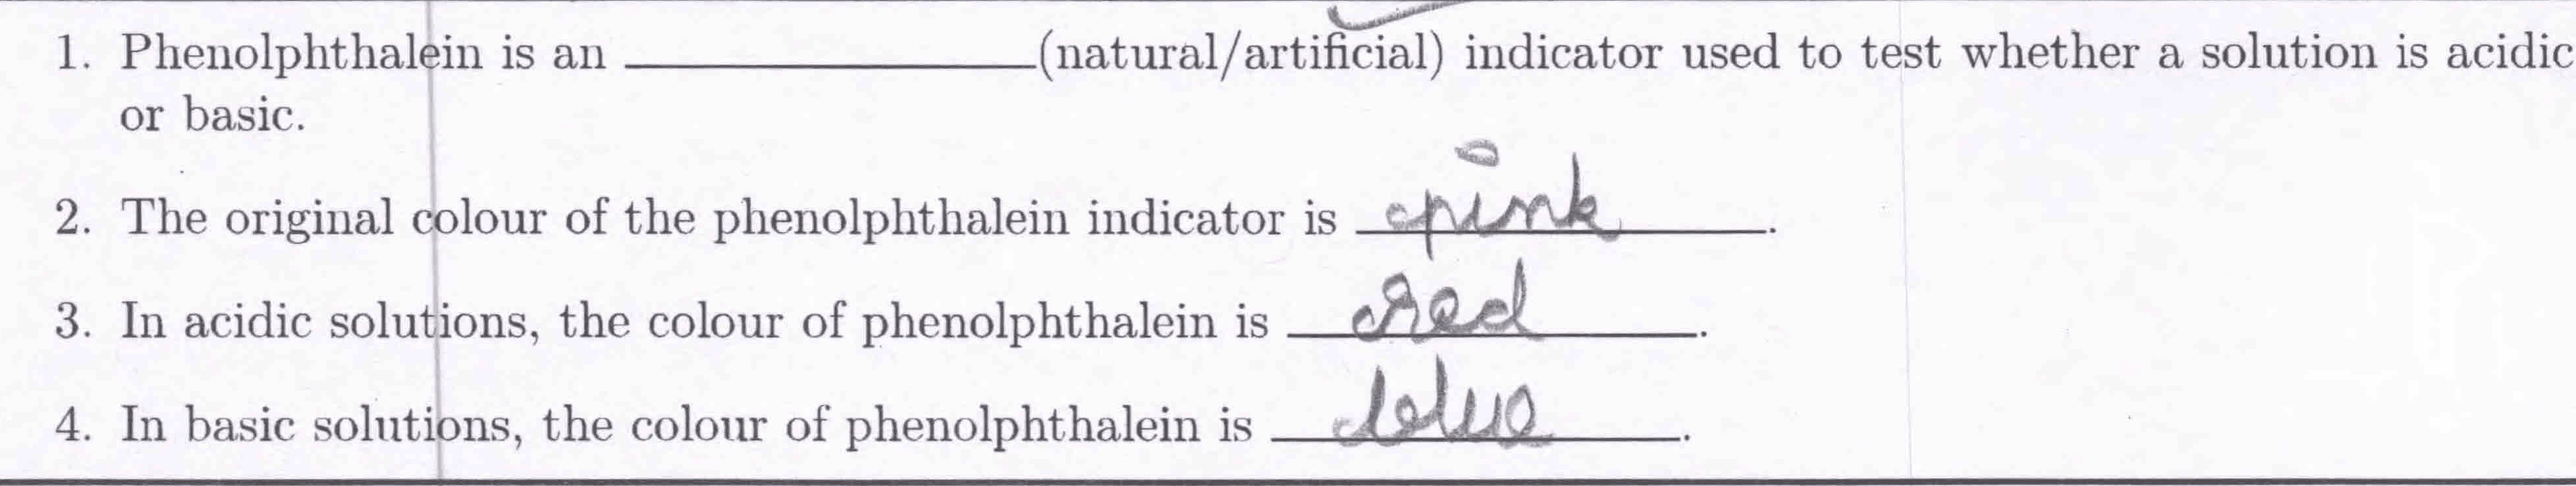
\includegraphics[width=4cm]{Q52_D117186_Science.png}}
    \end{minipage}
    \vspace{10pt}

    % Image: Q52_D117188_Science.png - Scaled height: 3.53mm
    \begin{minipage}{\linewidth}
    \RaggedRight\textbf{\tiny \highred{Anjali Mishra [E]}} \\ 
    \vspace{4.00pt}\fcolorbox{blue}{white}{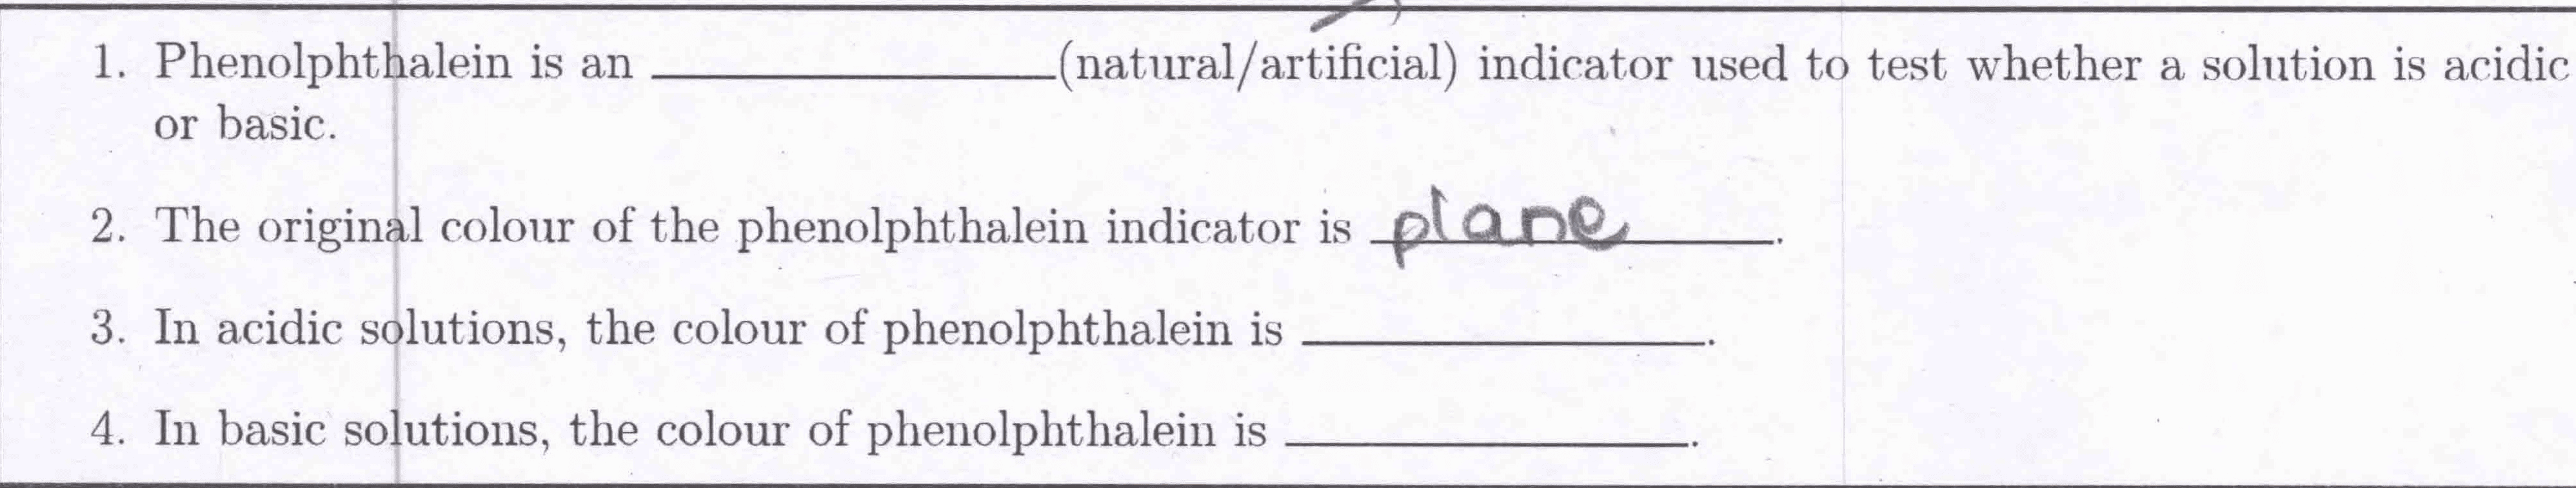
\includegraphics[width=4cm]{Q52_D117188_Science.png}}
    \end{minipage}
    \vspace{10pt}

    % Image: Q52_D117192_Science.png - Scaled height: 3.44mm
    \begin{minipage}{\linewidth}
    \RaggedRight\textbf{\tiny \highgreen{Shri Yashini P [C]}} \\ 
    \vspace{4.00pt}\fcolorbox{blue}{white}{\includegraphics[width=4cm]{Q52_D117192_Science.png}}
    \end{minipage}
    \vspace{10pt}

    % Image: Q52_D117194_Science.png - Scaled height: 3.50mm
    \begin{minipage}{\linewidth}
    \RaggedRight\textbf{\tiny \highgreen{Tharsika S [C]}} \\ 
    \vspace{4.00pt}\fcolorbox{blue}{white}{\includegraphics[width=4cm]{Q52_D117194_Science.png}}
    \end{minipage}
    \vspace{10pt}

    % Image: Q52_D117198_Science.png - Scaled height: 3.44mm
    \begin{minipage}{\linewidth}
    \RaggedRight\textbf{\tiny \highgreen{Eniyan E [C]}} \\ 
    \vspace{4.00pt}\fcolorbox{blue}{white}{\includegraphics[width=4cm]{Q52_D117198_Science.png}}
    \end{minipage}
    \vspace{10pt}

    % Image: Q52_D117202_Science.png - Scaled height: 3.52mm
    \begin{minipage}{\linewidth}
    \RaggedRight\textbf{\tiny \highred{Sashaanth S K [B]}} \\ 
    \vspace{4.00pt}\fcolorbox{blue}{white}{\includegraphics[width=4cm]{Q52_D117202_Science.png}}
    \end{minipage}
    \vspace{10pt}

    % Image: Q52_D117205_Science.png - Scaled height: 3.50mm
    \begin{minipage}{\linewidth}
    \RaggedRight\textbf{\tiny \highred{Divya Dharshini R J [D]}} \\ 
    \vspace{4.00pt}\fcolorbox{blue}{white}{\includegraphics[width=4cm]{Q52_D117205_Science.png}}
    \end{minipage}
    \vspace{10pt}

    % Image: Q52_D117206_Science.png - Scaled height: 3.48mm
    \begin{minipage}{\linewidth}
    \RaggedRight\textbf{\tiny \highred{Hansika S R [B]}} \\ 
    \vspace{4.00pt}\fcolorbox{blue}{white}{\includegraphics[width=4cm]{Q52_D117206_Science.png}}
    \end{minipage}
    \vspace{10pt}

    \end{multicols}
\end{frame}




\begin{frame}[shrink=0.1,label=QPC7QC7S07 - DT - Q8]{Q11 [5. Physical and Chemical Changes]}
\vspace{-0.2cm}
\mcqtextbottomOneFour{
  questionnumber={11}, 
  questionTag={C7S07 – DT – Q8 }, 
  questiontext={An iron rod used for constructing a house was left unnoticed for a long time in the open air. When seen after a long time, it has changed its colour and appears without its usual lustrous property. What might be the reason for this?},
  optionA={Rusting },
  optionB={Crystallisation },
  optionC={Melting },
  optionD={Galvanisation },
  correctoption={A},
}

\begin{minipage}{\linewidth}
\hspace{1cm}
\centering
\tiny
\renewcommand{\arraystretch}{1.25}
\begin{tabular}{|M{1.2cm}|M{0.8cm}|M{0.8cm}|M{0.8cm}|M{0.8cm}|M{0.8cm}|}
\hline
Option & \cellcolor{cellgreen} A (\ding{51}) & B (\ding{55}) & C (\ding{55}) & D (\ding{55}) & E \\ 
\hline
7 A & \highgreen{88\%} & \highno{6\%} & \highno{6\%} & \highno{0\%} & \highno{0\%} \\ 
 \hline 
7 B & \highgreen{93\%} & \highno{7\%} & \highno{0\%} & \highno{0\%} & \highno{0\%} \\ \hline
\end{tabular}
\end{minipage}

\end{frame}
% \input{4. PPT/6. My Answer/Science/C7/117_C7S - Q11}


\begin{frame}[shrink=0.1,label=QPC7QC7S07 - DT - Q6]{Q12 [5. Physical and Chemical Changes]}
\vspace{-0.2cm}
\mcqtextbottomOneFour{
  questionnumber={12}, 
  questionTag={C7S07 – DT – Q6 }, 
  questiontext={Which of the following is not an example of a chemical change?},
  optionA={Boiled egg},
  optionB={Photosynthesis},
  optionC={Burning of paper},
  optionD={Freezing water},
  correctoption={D},
}

\begin{minipage}{\linewidth}
\hspace{1cm}
\centering
\tiny
\renewcommand{\arraystretch}{1.25}
\begin{tabular}{|M{1.2cm}|M{0.8cm}|M{0.8cm}|M{0.8cm}|M{0.8cm}|M{0.8cm}|}
\hline
Option & A (\ding{55}) & B (\ding{55}) & C (\ding{55}) & \cellcolor{cellgreen} D (\ding{51}) & E \\ 
\hline
7 A & \highno{6\%} & \highno{19\%} & \highno{50\%} & \highred{25\%} & \highno{0\%} \\ 
 \hline 
7 B & \highno{21\%} & \highno{50\%} & \highno{29\%} & \highred{0\%} & \highno{0\%} \\ \hline
\end{tabular}
\end{minipage}

\end{frame}
% \input{4. PPT/6. My Answer/Science/C7/117_C7S - Q12}


\begin{frame}[shrink=0.1,label=QPC7QC7S07 - DT - Q4]{Q29 [5. Physical and Chemical Changes]}
\vspace{-0.2cm}
\mcqtextbottomOneFour{
  questionnumber={29}, 
  questionTag={C7S07 – DT – Q4 }, 
  questiontext={Magnesium ribbon always burns with a brilliant white light. This combustion is possible because of the reaction of magnesium ribbon with \rule{60pt}{0.1pt}.},
  optionA={ Water},
  optionB={ Air},
  optionC={Base},
  optionD={Acid},
  correctoption={B},
}

\begin{minipage}{\linewidth}
\hspace{1cm}
\centering
\tiny
\renewcommand{\arraystretch}{1.25}
\begin{tabular}{|M{1.2cm}|M{0.8cm}|M{0.8cm}|M{0.8cm}|M{0.8cm}|M{0.8cm}|}
\hline
Option & A (\ding{55}) & \cellcolor{cellgreen} B (\ding{51}) & C (\ding{55}) & D (\ding{55}) & E \\ 
\hline
7 A & \highno{0\%} & \highno{56\%} & \highno{0\%} & \highno{44\%} & \highno{0\%} \\ 
 \hline 
7 B & \highno{14\%} & \highred{21\%} & \highno{29\%} & \highno{36\%} & \highno{0\%} \\ \hline
\end{tabular}
\end{minipage}

\end{frame}
% \input{4. PPT/6. My Answer/Science/C7/117_C7S - Q29}


\begin{frame}[shrink=0.1,label=QPC7QC7S07 - DT - Q13]{Q56 [5. Physical and Chemical Changes]}
\vspace{-0.2cm}

\matextbottomOneFour{
myanswerquestion={Fill in the blanks based on the physical and chemical change},
myanswercontent={\begin{enumerate}
    \item A \rule{80pt}{0.5pt} change affects only the physical properties of a substance without forming a new substance.
    \item A \rule{80pt}{0.5pt} change results in the formation of a new substance with different properties.
    \item Burning wood is an example of a \rule{80pt}{0.5pt} change because a new substance is produced.
\end{enumerate}
},
questionnumber={56}, 
questionTag={C7S07 - DT - Q13}, 
questiontext={What kind of change occurs when ice cream melts after being left outside for a while?},
optionA={Chemical change},
optionB={Physical change},
optionC={Biological change},
optionD={Periodic change},
correctoption={B},
}




\begin{minipage}{\linewidth}
\hspace{1cm}
\centering
\tiny
\renewcommand{\arraystretch}{1.25}
\begin{tabular}{|M{1.2cm}|M{0.8cm}|M{0.8cm}|M{0.8cm}|M{0.8cm}|M{0.8cm}|}
\hline
Option & A (\ding{55}) & \cellcolor{cellgreen} B (\ding{51}) & C (\ding{55}) & D (\ding{55}) & E \\ 
\hline
7 A & \highno{44\%} & \highno{44\%} & \highno{6\%} & \highno{0\%} & \highno{6\%} \\ 
 \hline 
7 B & \highno{43\%} & \highno{43\%} & \highno{0\%} & \highno{14\%} & \highno{0\%} \\ \hline
\end{tabular}
\end{minipage}

\end{frame}
\begin{frame}{Q56 - My Answer Responses}
    \vspace{-0.6cm}
    \begin{multicols}{3}

    % Image: Q56_D117179_Science.png - Scaled height: 1.96mm
    \begin{minipage}{\linewidth}
    \RaggedRight\textbf{\tiny \highred{Kallis K [A]}} \\ 
    \vspace{4.00pt}\fcolorbox{blue}{white}{\includegraphics[width=4cm]{Q56_D117179_Science.png}}
    \end{minipage}
    \vspace{10pt}

    % Image: Q56_D117180_Science.png - Scaled height: 2.72mm
    \begin{minipage}{\linewidth}
    \RaggedRight\textbf{\tiny \highred{Rohith Vishnu N [A]}} \\ 
    \vspace{4.00pt}\fcolorbox{blue}{white}{\includegraphics[width=4cm]{Q56_D117180_Science.png}}
    \end{minipage}
    \vspace{10pt}

    % Image: Q56_D117184_Science.png - Scaled height: 2.74mm
    \begin{minipage}{\linewidth}
    \RaggedRight\textbf{\tiny \highred{Sudharshan T K [E]}} \\ 
    \vspace{4.00pt}\fcolorbox{blue}{white}{\includegraphics[width=4cm]{Q56_D117184_Science.png}}
    \end{minipage}
    \vspace{10pt}

    % Image: Q56_D117186_Science.png - Scaled height: 2.36mm
    \begin{minipage}{\linewidth}
    \RaggedRight\textbf{\tiny \highgreen{Yashwanth M [B]}} \\ 
    \vspace{4.00pt}\fcolorbox{blue}{white}{\includegraphics[width=4cm]{Q56_D117186_Science.png}}
    \end{minipage}
    \vspace{10pt}

    % Image: Q56_D117188_Science.png - Scaled height: 2.62mm
    \begin{minipage}{\linewidth}
    \RaggedRight\textbf{\tiny \highgreen{Anjali Mishra [B]}} \\ 
    \vspace{4.00pt}\fcolorbox{blue}{white}{\includegraphics[width=4cm]{Q56_D117188_Science.png}}
    \end{minipage}
    \vspace{10pt}

    % Image: Q56_D117190_Science.png - Scaled height: 2.32mm
    \begin{minipage}{\linewidth}
    \RaggedRight\textbf{\tiny \highred{Mithra J R [A]}} \\ 
    \vspace{4.00pt}\fcolorbox{blue}{white}{\includegraphics[width=4cm]{Q56_D117190_Science.png}}
    \end{minipage}
    \vspace{10pt}

    % Image: Q56_D117192_Science.png - Scaled height: 4.64mm
    \begin{minipage}{\linewidth}
    \RaggedRight\textbf{\tiny \highgreen{Shri Yashini P [B]}} \\ 
    \vspace{4.00pt}\fcolorbox{blue}{white}{\includegraphics[width=4cm]{Q56_D117192_Science.png}}
    \end{minipage}
    \vspace{10pt}

    % Image: Q56_D117208_Science.png - Scaled height: 2.58mm
    \begin{minipage}{\linewidth}
    \RaggedRight\textbf{\tiny \highred{Karnika S E A [A]}} \\ 
    \vspace{4.00pt}\fcolorbox{blue}{white}{\includegraphics[width=4cm]{Q56_D117208_Science.png}}
    \end{minipage}
    \vspace{10pt}

    % Image: Q56_D117212_Science.png - Scaled height: 2.68mm
    \begin{minipage}{\linewidth}
    \RaggedRight\textbf{\tiny \highgreen{Tanvisha V [B]}} \\ 
    \vspace{4.00pt}\fcolorbox{blue}{white}{\includegraphics[width=4cm]{Q56_D117212_Science.png}}
    \end{minipage}
    \vspace{10pt}

    \end{multicols}
\end{frame}




\begin{frame}[shrink=0.1,label=QPC7QC7S11 - DT - Q4]{Q14 [6. Respiration in Organisms]}
\vspace{-0.2cm}
\mcqtextbottomOneFour{
  questionnumber={14}, 
  questionTag={C7S11 – DT – Q4}, 
  questiontext={Name the gas inhaled during respiration \rule{80pt}{0.1pt}.},
  optionA={Oxygen},
  optionB={Carbon dioxide},
  optionC={Nitrogen},
  optionD={Glucose},
  correctoption={A},
}

\begin{minipage}{\linewidth}
\hspace{1cm}
\centering
\tiny
\renewcommand{\arraystretch}{1.25}
\begin{tabular}{|M{1.2cm}|M{0.8cm}|M{0.8cm}|M{0.8cm}|M{0.8cm}|M{0.8cm}|}
\hline
Option & \cellcolor{cellgreen} A (\ding{51}) & B (\ding{55}) & C (\ding{55}) & D (\ding{55}) & E \\ 
\hline
7 A & \highgreen{100\%} & \highno{0\%} & \highno{0\%} & \highno{0\%} & \highno{0\%} \\ 
 \hline 
7 B & \highno{71\%} & \highno{14\%} & \highno{0\%} & \highno{14\%} & \highno{0\%} \\ \hline
\end{tabular}
\end{minipage}

\end{frame}
% \input{4. PPT/6. My Answer/Science/C7/117_C7S - Q14}


\begin{frame}[shrink=0.1,label=QPC7QC7S11 - DT - Q10]{Q17 [6. Respiration in Organisms]}
\vspace{-0.2cm}
\mcqtextbottomOneFour{
  questionnumber={17}, 
  questionTag={C7S11 – DT – Q10}, 
  questiontext={Which part helps in the exchange of oxygen and carbon dioxide in plants? },
  optionA={Root},
  optionB={Stomata},
  optionC={Stem},
  optionD={Branches},
  correctoption={B},
}

\begin{minipage}{\linewidth}
\hspace{1cm}
\centering
\tiny
\renewcommand{\arraystretch}{1.25}
\begin{tabular}{|M{1.2cm}|M{0.8cm}|M{0.8cm}|M{0.8cm}|M{0.8cm}|M{0.8cm}|}
\hline
Option & A (\ding{55}) & \cellcolor{cellgreen} B (\ding{51}) & C (\ding{55}) & D (\ding{55}) & E \\ 
\hline
7 A & \highno{0\%} & \highgreen{88\%} & \highno{6\%} & \highno{6\%} & \highno{0\%} \\ 
 \hline 
7 B & \highno{0\%} & \highgreen{100\%} & \highno{0\%} & \highno{0\%} & \highno{0\%} \\ \hline
\end{tabular}
\end{minipage}

\end{frame}
% \input{4. PPT/6. My Answer/Science/C7/117_C7S - Q17}


\begin{frame}[shrink=0.1,label=QPC7QC7S11 - DT - Q8]{Q39 [6. Respiration in Organisms]}
\vspace{-0.2cm}
\mcqtextbottomOneFour{
  questionnumber={39}, 
  questionTag={C7S11 – DT – Q8 }, 
  questiontext={Name the part that helps the fish to breathe under the water.},
  optionA={Gills},
  optionB={Lungs},
  optionC={Spiracles},
  optionD={Skin},
  correctoption={A},
}

\begin{minipage}{\linewidth}
\hspace{1cm}
\centering
\tiny
\renewcommand{\arraystretch}{1.25}
\begin{tabular}{|M{1.2cm}|M{0.8cm}|M{0.8cm}|M{0.8cm}|M{0.8cm}|M{0.8cm}|}
\hline
Option & \cellcolor{cellgreen} A (\ding{51}) & B (\ding{55}) & C (\ding{55}) & D (\ding{55}) & E \\ 
\hline
7 A & \highgreen{94\%} & \highno{6\%} & \highno{0\%} & \highno{0\%} & \highno{0\%} \\ 
 \hline 
7 B & \highgreen{86\%} & \highno{7\%} & \highno{0\%} & \highno{0\%} & \highno{7\%} \\ \hline
\end{tabular}
\end{minipage}

\end{frame}
% \input{4. PPT/6. My Answer/Science/C7/117_C7S - Q39}


\begin{frame}[shrink=0.1,label=QPC7QC7S11 - DT - Q23]{Q45 [6. Respiration in Organisms]}
\vspace{-0.2cm}

\mcqtextbottomOneFour{
  questionnumber={45}, 
  questionTag={C7S11 – DT – Q23}, 
  questiontext={Identify the living organisms that respire through lungs.},
  optionA={\adjustbox{scale=\scalefactor}{\includegraphics[width=2.75cm,height=2cm]{C7S11 – DT – Q23i.png}}},
  optionB={\adjustbox{scale=\scalefactor}{\includegraphics[width=2.75cm,height=2cm]{C7S11 – DT – Q23ii.png}}},
  optionC={\adjustbox{scale=\scalefactor}{\includegraphics[width=2.75cm,height=2cm]{C7S11 – DT – Q23iii.png}}},
  optionD={\adjustbox{scale=\scalefactor}{\includegraphics[width=2.75cm,height=2cm]{C7S11 – DT – Q23iv.png}}},
  correctoption={B},
}


\begin{minipage}{\linewidth}
\hspace{1cm}
\centering
\tiny
\renewcommand{\arraystretch}{1.25}
\begin{tabular}{|M{1.2cm}|M{0.8cm}|M{0.8cm}|M{0.8cm}|M{0.8cm}|M{0.8cm}|}
\hline
Option & A (\ding{55}) & \cellcolor{cellgreen} B (\ding{51}) & C (\ding{55}) & D (\ding{55}) & E \\ 
\hline
7 A & \highno{0\%} & \highgreen{94\%} & \highno{6\%} & \highno{0\%} & \highno{0\%} \\ 
 \hline 
7 B & \highno{0\%} & \highgreen{79\%} & \highno{0\%} & \highno{21\%} & \highno{0\%} \\ \hline
\end{tabular}
\end{minipage}

\end{frame}
% \input{4. PPT/6. My Answer/Science/C7/117_C7S - Q45}


\begin{frame}[shrink=0.1,label=QPC7QC7S11 - DT - Q9]{Q48 [6. Respiration in Organisms]}
\vspace{-0.2cm}
\mcqtextbottomTwoTwo{
  questionnumber={48}, 
  questionTag={C7S11 – DT – Q9 }, 
  questiontext={Find the correct movement of air during respiration in humans.},
  optionA={Nostril $\rightarrow$ Trachea $\rightarrow$ Pharynx $\rightarrow$ Lungs},
  optionB={Nostril $\rightarrow$ Pharynx $\rightarrow$ Lungs $\rightarrow$ Trachea},
  optionC={Nostril $\rightarrow$ Lungs $\rightarrow$ Pharynx $\rightarrow$ Trachea},
  optionD={Nostril $\rightarrow$ Pharynx $\rightarrow$ Trachea $\rightarrow$ Lungs},
  correctoption={D},
}

\begin{minipage}{\linewidth}
\hspace{1cm}
\centering
\tiny
\renewcommand{\arraystretch}{1.25}
\begin{tabular}{|M{1.2cm}|M{0.8cm}|M{0.8cm}|M{0.8cm}|M{0.8cm}|M{0.8cm}|}
\hline
Option & A (\ding{55}) & B (\ding{55}) & C (\ding{55}) & \cellcolor{cellgreen} D (\ding{51}) & E \\ 
\hline
7 A & \highno{38\%} & \highno{19\%} & \highno{0\%} & \highred{38\%} & \highno{6\%} \\ 
 \hline 
7 B & \highno{57\%} & \highno{7\%} & \highno{14\%} & \highred{21\%} & \highno{0\%} \\ \hline
\end{tabular}
\end{minipage}

\end{frame}
% \input{4. PPT/6. My Answer/Science/C7/117_C7S - Q48}


\begin{frame}[shrink=15,label=QPC7QC7S11 - DT - Q26]{Q51 [6. Respiration in Organisms]}
\vspace{-0.2cm}

\matextbottomFourOne{
myanswerquestion={Fill in the blanks based on breathing rate.},
myanswercontent={\begin{enumerate}
    \item Breathing rate is the number of \rule{80pt}{0.5pt} per minute.
    \item During sleep, the breathing rate is \rule{80pt}{0.5pt}(higher/lower) because the energy requirement is \rule{80pt}{0.5pt}(higher/lower). 
     \item During heavy work, the oxygen demand is \rule{80pt}{0.5pt}(higher/lower) for energy production.
\end{enumerate}},
questionnumber={51}, 
questionTag={C7S11 - DT - Q26},
questiontext={Whose breathing will be faster?\\
\tikzset{every picture/.style={line width=0.75pt,scale=\scalefactor}}
\begin{tikzpicture}[x=0.75pt,y=0.75pt,yscale=-1,xscale=1]
\draw (177.17,61.33) node  {\adjustbox{scale=\scalefactor}{\includegraphics[width=201.25pt,height=64.5pt]{C7S11 – DT – Q2 i.jpg}}};
\draw (467.17,59) node  {\adjustbox{scale=\scalefactor}{\includegraphics[width=211.92pt,height=68.5pt]{C7S11 – DT – Q2 ii.jpg}}};
\draw (23,11) node [anchor=north west][inner sep=0.75pt]   [align=left] {1)};
\draw (333,11) node [anchor=north west][inner sep=0.75pt]   [align=left] {2)};
\draw (90,61.33) node [anchor=north west][inner sep=0.75pt]   [align=left] {Raju reached his \\house by walking};
\draw (397.11,60) node [anchor=north west][inner sep=0.75pt]   [align=left] {Ravi reached his \\house by running};
\end{tikzpicture}},
optionA={Raju’s breathing will be faster},
optionB={Ravi’s breathing will be faster},
optionC={Faster breathing does not depend on walking or running},
optionD={None of the above}, 
correctoption={B},
}

\begin{minipage}{\linewidth}
\hspace{1cm}
\centering
\tiny
\renewcommand{\arraystretch}{1.25}
\begin{tabular}{|M{1.2cm}|M{0.8cm}|M{0.8cm}|M{0.8cm}|M{0.8cm}|M{0.8cm}|}
\hline
Option & A (\ding{55}) & \cellcolor{cellgreen} B (\ding{51}) & C (\ding{55}) & D (\ding{55}) & E \\ 
\hline
7 A & \highno{6\%} & \highgreen{88\%} & \highno{6\%} & \highno{0\%} & \highno{0\%} \\ 
 \hline 
7 B & \highno{7\%} & \highno{71\%} & \highno{14\%} & \highno{7\%} & \highno{0\%} \\ \hline
\end{tabular}
\end{minipage}

\end{frame}
\begin{frame}{Q51 - My Answer Responses}
    \vspace{-0.6cm}
    \begin{multicols}{3}

    % Image: Q51_D117179_Science.png - Scaled height: 2.66mm
    \begin{minipage}{\linewidth}
    \RaggedRight\textbf{\tiny \highgreen{Kallis K [B]}} \\ 
    \vspace{4.00pt}\fcolorbox{blue}{white}{\includegraphics[width=4cm]{Q51_D117179_Science.png}}
    \end{minipage}
    \vspace{10pt}

    % Image: Q51_D117180_Science.png - Scaled height: 2.73mm
    \begin{minipage}{\linewidth}
    \RaggedRight\textbf{\tiny \highgreen{Rohith Vishnu N [B]}} \\ 
    \vspace{4.00pt}\fcolorbox{blue}{white}{\includegraphics[width=4cm]{Q51_D117180_Science.png}}
    \end{minipage}
    \vspace{10pt}

    % Image: Q51_D117183_Science.png - Scaled height: 2.78mm
    \begin{minipage}{\linewidth}
    \RaggedRight\textbf{\tiny \highgreen{Srishravan N M [B]}} \\ 
    \vspace{4.00pt}\fcolorbox{blue}{white}{\includegraphics[width=4cm]{Q51_D117183_Science.png}}
    \end{minipage}
    \vspace{10pt}

    % Image: Q51_D117187_Science.png - Scaled height: 2.67mm
    \begin{minipage}{\linewidth}
    \RaggedRight\textbf{\tiny \highgreen{Aadhana S S [B]}} \\ 
    \vspace{4.00pt}\fcolorbox{blue}{white}{\includegraphics[width=4cm]{Q51_D117187_Science.png}}
    \end{minipage}
    \vspace{10pt}

    % Image: Q51_D117188_Science.png - Scaled height: 2.67mm
    \begin{minipage}{\linewidth}
    \RaggedRight\textbf{\tiny \highgreen{Anjali Mishra [B]}} \\ 
    \vspace{4.00pt}\fcolorbox{blue}{white}{\includegraphics[width=4cm]{Q51_D117188_Science.png}}
    \end{minipage}
    \vspace{10pt}

    % Image: Q51_D117191_Science.png - Scaled height: 2.74mm
    \begin{minipage}{\linewidth}
    \RaggedRight\textbf{\tiny \highgreen{Sharlin Maria T [B]}} \\ 
    \vspace{4.00pt}\fcolorbox{blue}{white}{\includegraphics[width=4cm]{Q51_D117191_Science.png}}
    \end{minipage}
    \vspace{10pt}

    % Image: Q51_D117199_Science.png - Scaled height: 2.72mm
    \begin{minipage}{\linewidth}
    \RaggedRight\textbf{\tiny \highgreen{Karthick V [B]}} \\ 
    \vspace{4.00pt}\fcolorbox{blue}{white}{\includegraphics[width=4cm]{Q51_D117199_Science.png}}
    \end{minipage}
    \vspace{10pt}

    % Image: Q51_D117208_Science.png - Scaled height: 2.71mm
    \begin{minipage}{\linewidth}
    \RaggedRight\textbf{\tiny \highgreen{Karnika S E A [B]}} \\ 
    \vspace{4.00pt}\fcolorbox{blue}{white}{\includegraphics[width=4cm]{Q51_D117208_Science.png}}
    \end{minipage}
    \vspace{10pt}

    % Image: Q51_D117211_Science.png - Scaled height: 2.76mm
    \begin{minipage}{\linewidth}
    \RaggedRight\textbf{\tiny \highgreen{Tanu Shree R S [B]}} \\ 
    \vspace{4.00pt}\fcolorbox{blue}{white}{\includegraphics[width=4cm]{Q51_D117211_Science.png}}
    \end{minipage}
    \vspace{10pt}

    % Image: Q51_D117212_Science.png - Scaled height: 2.74mm
    \begin{minipage}{\linewidth}
    \RaggedRight\textbf{\tiny \highgreen{Tanvisha V [B]}} \\ 
    \vspace{4.00pt}\fcolorbox{blue}{white}{\includegraphics[width=4cm]{Q51_D117212_Science.png}}
    \end{minipage}
    \vspace{10pt}

    \end{multicols}
\end{frame}




\begin{frame}[shrink=0.1,label=QPC7QC7S12 - DT - Q9]{Q5 [7. Transportation in Animals and Plants]}
\vspace{-0.2cm}
\mcqtextbottomFourOne{
  questionnumber={5}, 
  questionTag={C7S12 – DT – Q9},
  questiontext={Identify the direction of movement of nutrients in the xylem and phloem.},
  optionA={Upward direction – Xylem, Both upward and downward direction - Phloem},
  optionB={Upward direction – Phloem, Only downward direction - Xylem},
  optionC={Downward direction – Phloem, Upward direction - Xylem},
  optionD={Both upward and downward direction – Xylem, Upward direction – Phloem}, 
  correctoption={A},
}

\begin{minipage}{\linewidth}
\hspace{1cm}
\centering
\tiny
\renewcommand{\arraystretch}{1.25}
\begin{tabular}{|M{1.2cm}|M{0.8cm}|M{0.8cm}|M{0.8cm}|M{0.8cm}|M{0.8cm}|}
\hline
Option & \cellcolor{cellgreen} A (\ding{51}) & B (\ding{55}) & C (\ding{55}) & D (\ding{55}) & E \\ 
\hline
7 A & \highred{38\%} & \highno{56\%} & \highno{0\%} & \highno{6\%} & \highno{0\%} \\ 
 \hline 
7 B & \highred{21\%} & \highno{21\%} & \highno{14\%} & \highno{36\%} & \highno{7\%} \\ \hline
\end{tabular}
\end{minipage}

\end{frame}
% \input{4. PPT/6. My Answer/Science/C7/117_C7S - Q5}


\begin{frame}[shrink=0.1,label=QPC7QC7S12 - DT - Q24]{Q30 [7. Transportation in Animals and Plants]}
\vspace{-0.2cm}

\mcqtextbottomTwoTwo{
  questionnumber={30}, 
  questionTag={C7S12 - DT - Q24}, 
  questiontext={Why do doctor recommend dialysis for people who suffer from kidney failure? },
  optionA={To improve the functioning of the kidney. },
  optionB={To check the heart beat regularly.},
  optionC={To purify the blood.},
  optionD={To help the kidneys grow. },
  correctoption={C},
}


\begin{minipage}{\linewidth}
\hspace{1cm}
\centering
\tiny
\renewcommand{\arraystretch}{1.25}
\begin{tabular}{|M{1.2cm}|M{0.8cm}|M{0.8cm}|M{0.8cm}|M{0.8cm}|M{0.8cm}|}
\hline
Option & A (\ding{55}) & B (\ding{55}) & \cellcolor{cellgreen} C (\ding{51}) & D (\ding{55}) & E \\ 
\hline
7 A & \highno{44\%} & \highno{6\%} & \highred{31\%} & \highno{13\%} & \highno{6\%} \\ 
 \hline 
7 B & \highno{43\%} & \highno{7\%} & \highno{50\%} & \highno{0\%} & \highno{0\%} \\ \hline
\end{tabular}
\end{minipage}

\end{frame}
% \input{4. PPT/6. My Answer/Science/C7/117_C7S - Q30}


\begin{frame}[shrink=0.1,label=QPC7QC7S12 - DT - Q4]{Q46 [7. Transportation in Animals and Plants]}
\vspace{-0.2cm}
\mcqimgbottomOneFour{
  questionnumber={46}, 
  questionTag={C7S12 – DT – Q4}, 
  questiontext={Identify the correct way to measure the pulse.},
  optionA={C7S12 – DT – Q4i.png},
  optionB={C7S12 – DT – Q4ii.png},
  optionC={C7S12 – DT – Q4iii.png},
  optionD={C7S12 – DT – Q4iv.png},
  correctoption={C},
}

\begin{minipage}{\linewidth}
\hspace{1cm}
\centering
\tiny
\renewcommand{\arraystretch}{1.25}
\begin{tabular}{|M{1.2cm}|M{0.8cm}|M{0.8cm}|M{0.8cm}|M{0.8cm}|M{0.8cm}|}
\hline
Option & A (\ding{55}) & B (\ding{55}) & \cellcolor{cellgreen} C (\ding{51}) & D (\ding{55}) & E \\ 
\hline
7 A & \highno{0\%} & \highno{0\%} & \highgreen{100\%} & \highno{0\%} & \highno{0\%} \\ 
 \hline 
7 B & \highno{14\%} & \highno{14\%} & \highno{71\%} & \highno{0\%} & \highno{0\%} \\ \hline
\end{tabular}
\end{minipage}

\end{frame}
% \input{4. PPT/6. My Answer/Science/C7/117_C7S - Q46}


\begin{frame}[shrink=25,label=QPC7QC7S12 - DT - Q29]{Q53 [7. Transportation in Animals and Plants]}
\vspace{-0.2cm}

\maimgleftFourOne{
myanswerquestion={Complete the table based on the functions of the blood vessel.},
myanswercontent={\renewcommand{\arraystretch}{1.5}\begin{tabular} {|m{7cm}|m{3cm}|}
\hline
\textbf{\centering Function} & \textbf{Type of Blood Vessel}\\
\hline
Carries oxygen-poor blood from the heart to the lungs.  &  \\
\hline
Exchange oxygen, nutrients, and waste between blood and tissues. & Capillaries \\
\hline
Carries oxygen-poor blood from the body back to the heart. & \\
\hline
Carry oxygen-rich blood from the heart to different parts of the body.& \\
\hline
Carries oxygen-rich blood from the lungs to the heart. & \\
\hline
\end{tabular}\\},
questionnumber={53}, 
questionTag={C7S12 - DT - Q29},
questiontext={Identify the blood vessel that carries blood from the lungs to the heart.},
imgtabletikz = {\adjustbox{scale=\scalefactor}{\includegraphics[width=5.5cm, height=4.5cm]{C7S12 - DT - Q29.png}}},
optionA={Pulmonary artery },
optionB={Artery},
optionC={Pulmonary vein},
optionD={Vein},
correctoption={C},
leftmini={0.5},
rightmini={0.4},
}

\begin{minipage}{\linewidth}
\hspace{1cm}
\centering
\tiny
\renewcommand{\arraystretch}{1.25}
\begin{tabular}{|M{1.2cm}|M{0.8cm}|M{0.8cm}|M{0.8cm}|M{0.8cm}|M{0.8cm}|}
\hline
Option & A (\ding{55}) & B (\ding{55}) & \cellcolor{cellgreen} C (\ding{51}) & D (\ding{55}) & E \\ 
\hline
7 A & \highno{19\%} & \highno{31\%} & \highred{19\%} & \highno{25\%} & \highno{6\%} \\ 
 \hline 
7 B & \highno{7\%} & \highno{57\%} & \highred{21\%} & \highno{14\%} & \highno{0\%} \\ \hline
\end{tabular}
\end{minipage}

\end{frame}
\begin{frame}{Q53 - My Answer Responses}
    \vspace{-0.6cm}
    \begin{multicols}{2}

    % Image: Q53_D117179_Science.png - Scaled height: 4.90mm
    \begin{minipage}{\linewidth}
    \RaggedRight\textbf{\tiny \highred{Kallis K [B]}} \\ 
    \vspace{4.00pt}\fcolorbox{blue}{white}{\includegraphics[width=4cm]{Q53_D117179_Science.png}}
    \end{minipage}
    \vspace{10pt}

    % Image: Q53_D117183_Science.png - Scaled height: 4.91mm
    \begin{minipage}{\linewidth}
    \RaggedRight\textbf{\tiny \highred{Srishravan N M [B]}} \\ 
    \vspace{4.00pt}\fcolorbox{blue}{white}{\includegraphics[width=4cm]{Q53_D117183_Science.png}}
    \end{minipage}
    \vspace{10pt}

    % Image: Q53_D117187_Science.png - Scaled height: 4.77mm
    \begin{minipage}{\linewidth}
    \RaggedRight\textbf{\tiny \highred{Aadhana S S [B]}} \\ 
    \vspace{4.00pt}\fcolorbox{blue}{white}{\includegraphics[width=4cm]{Q53_D117187_Science.png}}
    \end{minipage}
    \vspace{10pt}

    % Image: Q53_D117199_Science.png - Scaled height: 4.90mm
    \begin{minipage}{\linewidth}
    \RaggedRight\textbf{\tiny \highred{Karthick V [B]}} \\ 
    \vspace{4.00pt}\fcolorbox{blue}{white}{\includegraphics[width=4cm]{Q53_D117199_Science.png}}
    \end{minipage}
    \vspace{10pt}

    % Image: Q53_D117203_Science.png - Scaled height: 4.78mm
    \begin{minipage}{\linewidth}
    \RaggedRight\textbf{\tiny \highred{Vibin A [A]}} \\ 
    \vspace{4.00pt}\fcolorbox{blue}{white}{\includegraphics[width=4cm]{Q53_D117203_Science.png}}
    \end{minipage}
    \vspace{10pt}

    % Image: Q53_D117211_Science.png - Scaled height: 4.85mm
    \begin{minipage}{\linewidth}
    \RaggedRight\textbf{\tiny \highred{Tanu Shree R S [B]}} \\ 
    \vspace{4.00pt}\fcolorbox{blue}{white}{\includegraphics[width=4cm]{Q53_D117211_Science.png}}
    \end{minipage}
    \vspace{10pt}

    \end{multicols}
\end{frame}




\begin{frame}[shrink=0.1,label=QPC7QC7S13 - DT - Q2]{Q9 [8. Reproduction in Plants]}
\vspace{-0.2cm}
\mcqimgleftFourOne{
  questionnumber={9}, 
  questionTag={C7S13 – DT – Q2},
  questiontext={Identify the marked part in the flower.},
  imgtabletikz= {

\tikzset{every picture/.style={line width=0.75pt,scale=\scalefactor}}
\begin{tikzpicture}[x=0.75pt,y=0.75pt,yscale=-1,xscale=1]
\draw (141,133.3) node  {\adjustbox{scale=\scalefactor}{\includegraphics[width=163.5pt,height=106.05pt]{C7S13 – DT – Q2.png}}};
\draw    (209,107) -- (293,107) ;
\draw [shift={(295,107)}, rotate = 180] [color={rgb, 255:red, 0; green, 0; blue, 0 }  ][line width=0.75]    (10.93,-3.29) .. controls (6.95,-1.4) and (3.31,-0.3) .. (0,0) .. controls (3.31,0.3) and (6.95,1.4) .. (10.93,3.29)   ;
\draw    (183.6,147) -- (291.44,147) ;
\draw [shift={(293.44,147)}, rotate = 180] [color={rgb, 255:red, 0; green, 0; blue, 0 }  ][line width=0.75]    (10.93,-3.29) .. controls (6.95,-1.4) and (3.31,-0.3) .. (0,0) .. controls (3.31,0.3) and (6.95,1.4) .. (10.93,3.29)   ;
\draw (307.6,95.4) node [anchor=north west][inner sep=0.75pt]   [align=left] {a};
\draw (306.8,138.6) node [anchor=north west][inner sep=0.75pt]   [align=left] {b};
\end{tikzpicture}
},
  optionA={a - Petal, b - Stamen },
  optionB={a - Sepal, b - Pistil },
  optionC={a - Stamen, b - Pistil },
  optionD={a - Pistil, b - Petal},
  correctoption={A},
  leftmini={0.6},
  rightmini={0.3},
}

\begin{minipage}{\linewidth}
\hspace{1cm}
\centering
\tiny
\renewcommand{\arraystretch}{1.25}
\begin{tabular}{|M{1.2cm}|M{0.8cm}|M{0.8cm}|M{0.8cm}|M{0.8cm}|M{0.8cm}|}
\hline
Option & \cellcolor{cellgreen} A (\ding{51}) & B (\ding{55}) & C (\ding{55}) & D (\ding{55}) & E \\ 
\hline
7 A & \highgreen{88\%} & \highno{0\%} & \highno{6\%} & \highno{0\%} & \highno{6\%} \\ 
 \hline 
7 B & \highgreen{86\%} & \highno{0\%} & \highno{14\%} & \highno{0\%} & \highno{0\%} \\ \hline
\end{tabular}
\end{minipage}

\end{frame}
% \input{4. PPT/6. My Answer/Science/C7/117_C7S - Q9}


\begin{frame}[shrink=0.1,label=QPC7QC7S13 - DT - Q6]{Q21 [8. Reproduction in Plants]}
\vspace{-0.2cm}
\mcqimgleftFourOne{
  questionnumber={21}, 
  questionTag={C7S13 – DT – Q6},
  questiontext={Identify the mode of reproduction that takes place in green coloured organism (algae) in water body.},
  imgtabletikz = { {\adjustbox{scale=\scalefactor}{\includegraphics[width=3cm,height=2.5cm]{C7S13 – DT – Q6.png}}} },
  optionA={Budding },
  optionB={Fragmentation },
  optionC={Spore formation },
  optionD={Pollination },
  correctoption={B},
  leftmini={0.5},
  rightmini={0.4},
}

\begin{minipage}{\linewidth}
\hspace{1cm}
\centering
\tiny
\renewcommand{\arraystretch}{1.25}
\begin{tabular}{|M{1.2cm}|M{0.8cm}|M{0.8cm}|M{0.8cm}|M{0.8cm}|M{0.8cm}|}
\hline
Option & A (\ding{55}) & \cellcolor{cellgreen} B (\ding{51}) & C (\ding{55}) & D (\ding{55}) & E \\ 
\hline
7 A & \highno{6\%} & \highno{63\%} & \highno{25\%} & \highno{0\%} & \highno{6\%} \\ 
 \hline 
7 B & \highno{29\%} & \highred{14\%} & \highno{43\%} & \highno{14\%} & \highno{0\%} \\ \hline
\end{tabular}
\end{minipage}

\end{frame}
% \input{4. PPT/6. My Answer/Science/C7/117_C7S - Q21}


\begin{frame}[shrink=0.1,label=QPC7QC7S13 - DT - Q9]{Q41 [8. Reproduction in Plants]}
\vspace{-0.2cm}
\mcqtextbottomTwoTwo{
  questionnumber={41}, 
  questionTag={C7S13 – DT – Q9}, 
  questiontext={Identify the type of pollination that takes place in the given pictures. \\ \medskip
\tikzset{every picture/.style={line width=0.75pt,scale=\scalefactor}} 
\hspace{3cm}
\begin{tikzpicture}[x=0.75pt,y=0.75pt,yscale=-1,xscale=1]
\draw (412,147.8) node  {\adjustbox{scale=\scalefactor}{\includegraphics[width=97.5pt,height=79.8pt]{C7S13 – DT – Q9ii.png}}};
\draw (168,141.8) node  {\adjustbox{scale=\scalefactor}{\includegraphics[width=196.5pt,height=88.8pt]{C7S13 – DT – Q9i.png}}};
\draw (58,73) node [anchor=north west][inner sep=0.75pt]   [align=left] {\textbf{A}};
\draw (338,73) node [anchor=north west][inner sep=0.75pt]   [align=left] {\textbf{B}};
\end{tikzpicture} 
},
  optionA={A - Self pollination, B - Cross pollination },
  optionB={A - Cross pollination, B - Self pollination },
  optionC={A - Self pollination, B - Self pollination },
  optionD={A - Cross pollination, B - Cross pollination },
  correctoption={B},
}

\begin{minipage}{\linewidth}
\hspace{1cm}
\centering
\tiny
\renewcommand{\arraystretch}{1.25}
\begin{tabular}{|M{1.2cm}|M{0.8cm}|M{0.8cm}|M{0.8cm}|M{0.8cm}|M{0.8cm}|}
\hline
Option & A (\ding{55}) & \cellcolor{cellgreen} B (\ding{51}) & C (\ding{55}) & D (\ding{55}) & E \\ 
\hline
7 A & \highno{0\%} & \highgreen{88\%} & \highno{0\%} & \highno{13\%} & \highno{0\%} \\ 
 \hline 
7 B & \highno{14\%} & \highgreen{86\%} & \highno{0\%} & \highno{0\%} & \highno{0\%} \\ \hline
\end{tabular}
\end{minipage}

\end{frame}
% \input{4. PPT/6. My Answer/Science/C7/117_C7S - Q41}


\begin{frame}[shrink=0.1,label=QPC7QC7S13 - DT - Q11]{Q59 [8. Reproduction in Plants]}
\vspace{-0.2cm}

\matextbottomOneFour{
myanswerquestion={Answer the following questions based on the reproduction in plants.},
myanswercontent={\begin{enumerate}
    \item  Plants that use their parts for reproduction instead of seeds are called \rule{100pt}{0.5pt}.
    \item Label the reproductive part of the given rose plant. 
\end{enumerate}
{\adjustbox{scale=\scalefactor}{\includegraphics[width=2.5cm,height=3.5cm]{C7S13 - DT - Q11.jpg}} \\}},
questionnumber={59}, 
  questionTag={C7S13 - DT - Q11}, 
  questiontext={Find the odd one based on the vegetative part of the plant.},
  optionA={Root },
  optionB={Stem},
  optionC={Flower},
  optionD={Leaf},
  correctoption={C}
}


\begin{minipage}{\linewidth}
\hspace{1cm}
\centering
\tiny
\renewcommand{\arraystretch}{1.25}
\begin{tabular}{|M{1.2cm}|M{0.8cm}|M{0.8cm}|M{0.8cm}|M{0.8cm}|M{0.8cm}|}
\hline
Option & A (\ding{55}) & B (\ding{55}) & \cellcolor{cellgreen} C (\ding{51}) & D (\ding{55}) & E \\ 
\hline
7 A & \highno{13\%} & \highno{13\%} & \highno{63\%} & \highno{6\%} & \highno{6\%} \\ 
 \hline 
7 B & \highno{14\%} & \highno{14\%} & \highred{29\%} & \highno{36\%} & \highno{7\%} \\ \hline
\end{tabular}
\end{minipage}

\end{frame}
\begin{frame}{Q59 - My Answer Responses}
    \vspace{-0.6cm}
    \begin{multicols}{3}

    % Image: Q59_D117179_Science.png - Scaled height: 4.74mm
    \begin{minipage}{\linewidth}
    \RaggedRight\textbf{\tiny \highgreen{Kallis K [C]}} \\ 
    \vspace{4.00pt}\fcolorbox{blue}{white}{\includegraphics[width=4cm]{Q59_D117179_Science.png}}
    \end{minipage}
    \vspace{10pt}

    % Image: Q59_D117180_Science.png - Scaled height: 5.26mm
    \begin{minipage}{\linewidth}
    \RaggedRight\textbf{\tiny \highgreen{Rohith Vishnu N [C]}} \\ 
    \vspace{4.00pt}\fcolorbox{blue}{white}{\includegraphics[width=4cm]{Q59_D117180_Science.png}}
    \end{minipage}
    \vspace{10pt}

    % Image: Q59_D117186_Science.png - Scaled height: 5.20mm
    \begin{minipage}{\linewidth}
    \RaggedRight\textbf{\tiny \highgreen{Yashwanth M [C]}} \\ 
    \vspace{4.00pt}\fcolorbox{blue}{white}{\includegraphics[width=4cm]{Q59_D117186_Science.png}}
    \end{minipage}
    \vspace{10pt}

    % Image: Q59_D117187_Science.png - Scaled height: 4.74mm
    \begin{minipage}{\linewidth}
    \RaggedRight\textbf{\tiny \highred{Aadhana S S [A]}} \\ 
    \vspace{4.00pt}\fcolorbox{blue}{white}{\includegraphics[width=4cm]{Q59_D117187_Science.png}}
    \end{minipage}
    \vspace{10pt}

    % Image: Q59_D117188_Science.png - Scaled height: 5.16mm
    \begin{minipage}{\linewidth}
    \RaggedRight\textbf{\tiny \highgreen{Anjali Mishra [C]}} \\ 
    \vspace{4.00pt}\fcolorbox{blue}{white}{\includegraphics[width=4cm]{Q59_D117188_Science.png}}
    \end{minipage}
    \vspace{10pt}

    % Image: Q59_D117203_Science.png - Scaled height: 4.66mm
    \begin{minipage}{\linewidth}
    \RaggedRight\textbf{\tiny \highred{Vibin A [A]}} \\ 
    \vspace{4.00pt}\fcolorbox{blue}{white}{\includegraphics[width=4cm]{Q59_D117203_Science.png}}
    \end{minipage}
    \vspace{10pt}

    % Image: Q59_D117210_Science.png - Scaled height: 5.48mm
    \begin{minipage}{\linewidth}
    \RaggedRight\textbf{\tiny \highgreen{Swathi Sree K M [C]}} \\ 
    \vspace{4.00pt}\fcolorbox{blue}{white}{\includegraphics[width=4cm]{Q59_D117210_Science.png}}
    \end{minipage}
    \vspace{10pt}

    % Image: Q59_D117211_Science.png - Scaled height: 4.63mm
    \begin{minipage}{\linewidth}
    \RaggedRight\textbf{\tiny \highred{Tanu Shree R S [D]}} \\ 
    \vspace{4.00pt}\fcolorbox{blue}{white}{\includegraphics[width=4cm]{Q59_D117211_Science.png}}
    \end{minipage}
    \vspace{10pt}

    % Image: Q59_D117212_Science.png - Scaled height: 5.10mm
    \begin{minipage}{\linewidth}
    \RaggedRight\textbf{\tiny \highred{Tanvisha V [A]}} \\ 
    \vspace{4.00pt}\fcolorbox{blue}{white}{\includegraphics[width=4cm]{Q59_D117212_Science.png}}
    \end{minipage}
    \vspace{10pt}

    \end{multicols}
\end{frame}




\begin{frame}[shrink=0.1,label=QPC7QC7S14 - DT - Q2]{Q22 [9. Motion and Time]}
\vspace{-0.2cm}
  \mcqtextbottomFourOne{
  questionnumber={22},
  questionTag={C7S14 – DT – Q2},
  questiontext={Look at the given pictures, and identify the type of motion.
  
  \tikzset{every picture/.style={line width=0.75pt,scale=\scalefactor}} 
  \hspace{1.5cm}
\begin{tikzpicture}[x=0.75pt,y=0.75pt,yscale=-1,xscale=1]
\draw (129.27,131.42) node  {\adjustbox{scale=\scalefactor}{\includegraphics[width=75pt,height=65pt]{C7S14 – DT – Q2i.png}}};
\draw (328.77,131.7) node  {\adjustbox{scale=\scalefactor}{\includegraphics[width=75pt,height=65pt]{C7S14 – DT – Q2ii.png}}};
\draw (520.73,135.18) node  {\adjustbox{scale=\scalefactor}{\includegraphics[width=75pt,height=65pt]{C7S14 – DT – Q2iii.png}}};
\draw (46,185) node [anchor=north west][inner sep=0.75pt]   [align=left] {A - Motion while playing \\Ring a ring o roses };
\draw (247,185) node [anchor=north west][inner sep=0.75pt]   [align=left] {B - Movement of light \\ray};
\draw (443.56,185) node [anchor=north west][inner sep=0.75pt]   [align=left] {C - Movement of seconds \\hand in clock };
\end{tikzpicture}},
  optionA={A-Circular motion, B-Periodic motion, C-Circular motion},
  optionB={A-Circular motion, B-Rectilinear motion, C-Periodic motion},
  optionC={A-Rectilinear motion, B-Periodic motion, C-Circular motion},
  optionD={A-Periodic motion, B-Rectilinear motion, C-Rectilinear motion},
  correctoption={B},
}

\begin{minipage}{\linewidth}
\hspace{1cm}
\centering
\tiny
\renewcommand{\arraystretch}{1.25}
\begin{tabular}{|M{1.2cm}|M{0.8cm}|M{0.8cm}|M{0.8cm}|M{0.8cm}|M{0.8cm}|}
\hline
Option & A (\ding{55}) & \cellcolor{cellgreen} B (\ding{51}) & C (\ding{55}) & D (\ding{55}) & E \\ 
\hline
7 A & \highno{31\%} & \highno{63\%} & \highno{6\%} & \highno{0\%} & \highno{0\%} \\ 
 \hline 
7 B & \highno{57\%} & \highred{36\%} & \highno{0\%} & \highno{0\%} & \highno{7\%} \\ \hline
\end{tabular}
\end{minipage}

\end{frame}
% \input{4. PPT/6. My Answer/Science/C7/117_C7S - Q22}


\begin{frame}[shrink=0.1,label=QPC7QC7S14 - DT - Q10]{Q38 [9. Motion and Time]}
\vspace{-0.2cm}
\mcqimgleftFourOne{
  questionnumber={38}, 
  questionTag={C7S14 – DT – Q10 },
  questiontext={Find out the coordinates of the point ‘Q’ from the given distance-time graph.},
  imgtabletikz = { {\adjustbox{scale=\scalefactor}{\includegraphics[width=5cm,height=4cm]{C7S14 – DT – Q10 .jpg}}} },
  optionA={(16, 4)},
  optionB={(4, 16)},
  optionC={(8, 24)},
  optionD={(2, 16)},
  correctoption={B},
  leftmini={0.5},
  rightmini={0.4},
}

\begin{minipage}{\linewidth}
\hspace{1cm}
\centering
\tiny
\renewcommand{\arraystretch}{1.25}
\begin{tabular}{|M{1.2cm}|M{0.8cm}|M{0.8cm}|M{0.8cm}|M{0.8cm}|M{0.8cm}|}
\hline
Option & A (\ding{55}) & \cellcolor{cellgreen} B (\ding{51}) & C (\ding{55}) & D (\ding{55}) & E \\ 
\hline
7 A & \highno{81\%} & \highred{13\%} & \highno{0\%} & \highno{6\%} & \highno{0\%} \\ 
 \hline 
7 B & \highno{57\%} & \highred{21\%} & \highno{14\%} & \highno{7\%} & \highno{0\%} \\ \hline
\end{tabular}
\end{minipage}

\end{frame}
% \input{4. PPT/6. My Answer/Science/C7/117_C7S - Q38}


\begin{frame}[shrink=0.1,label=QPC7QC7S14 - DT - Q9]{Q42 [9. Motion and Time]}
\vspace{-0.2cm}
\mcqtextbottomOneFour{
  questionnumber={42}, 
  questionTag={C7S14 – DT – Q9}, 
  questiontext={Identify the origin coordinates from the given graphs.\\
  \adjustbox{scale=\scalefactor}{\includegraphics[width=16cm,height=3.2cm]{C7S14 – DT – Q9 .jpg}}
  },
  optionA={A},
  optionB={B},
  optionC={C},
  optionD={D},
  correctoption={D},
}

\begin{minipage}{\linewidth}
\hspace{1cm}
\centering
\tiny
\renewcommand{\arraystretch}{1.25}
\begin{tabular}{|M{1.2cm}|M{0.8cm}|M{0.8cm}|M{0.8cm}|M{0.8cm}|M{0.8cm}|}
\hline
Option & A (\ding{55}) & B (\ding{55}) & C (\ding{55}) & \cellcolor{cellgreen} D (\ding{51}) & E \\ 
\hline
7 A & \highno{0\%} & \highno{25\%} & \highno{0\%} & \highno{75\%} & \highno{0\%} \\ 
 \hline 
7 B & \highno{14\%} & \highno{14\%} & \highno{21\%} & \highno{50\%} & \highno{0\%} \\ \hline
\end{tabular}
\end{minipage}

\end{frame}
% \input{4. PPT/6. My Answer/Science/C7/117_C7S - Q42}


\begin{frame}[shrink=0.1,label=QPC7QC7S14 - DT - Q4]{Q55 [9. Motion and Time]}
\vspace{-0.2cm}
\mcqtextbottomOneFour{
  questionnumber={55}, 
  questionTag={C7S14 – DT – Q4 }, 
  questiontext={It took a minute and a half for a dog to cover 270 m. Find the speed of the dog.},
  optionA={30 km/hr},
  optionB={3 m/s},
  optionC={9 m/s},
  optionD={90 m/s },
  correctoption={B},
}

\begin{minipage}{\linewidth}
\hspace{1cm}
\centering
\tiny
\renewcommand{\arraystretch}{1.25}
\begin{tabular}{|M{1.2cm}|M{0.8cm}|M{0.8cm}|M{0.8cm}|M{0.8cm}|M{0.8cm}|}
\hline
Option & A (\ding{55}) & \cellcolor{cellgreen} B (\ding{51}) & C (\ding{55}) & D (\ding{55}) & E \\ 
\hline
7 A & \highno{6\%} & \highred{38\%} & \highno{44\%} & \highno{13\%} & \highno{0\%} \\ 
 \hline 
7 B & \highno{7\%} & \highred{36\%} & \highno{36\%} & \highno{21\%} & \highno{0\%} \\ \hline
\end{tabular}
\end{minipage}

\end{frame}
% \input{4. PPT/6. My Answer/Science/C7/117_C7S - Q55}


\begin{frame}[shrink=0.1,label=QPC7QC7S15 - DT - Q4]{Q20 [10. Electric Current and Its Effects]}
\vspace{-0.2cm}
\mcqtextbottomTwoTwo{
  questionnumber={20}, 
  questionTag={C7S15 – DT – Q4}, 
  questiontext={What happens when electric current flows through a wire placed near a compass?},
  optionA={Compass cools down.},
  optionB={Compass needle breaks.},
  optionC={Compass needle deflects.},
  optionD={Compass becomes hot.},
  correctoption={C},
}

\begin{minipage}{\linewidth}
\hspace{1cm}
\centering
\tiny
\renewcommand{\arraystretch}{1.25}
\begin{tabular}{|M{1.2cm}|M{0.8cm}|M{0.8cm}|M{0.8cm}|M{0.8cm}|M{0.8cm}|}
\hline
Option & A (\ding{55}) & B (\ding{55}) & \cellcolor{cellgreen} C (\ding{51}) & D (\ding{55}) & E \\ 
\hline
7 A & \highno{0\%} & \highno{0\%} & \highgreen{100\%} & \highno{0\%} & \highno{0\%} \\ 
 \hline 
7 B & \highno{0\%} & \highno{7\%} & \highgreen{93\%} & \highno{0\%} & \highno{0\%} \\ \hline
\end{tabular}
\end{minipage}

\end{frame}
% \input{4. PPT/6. My Answer/Science/C7/117_C7S - Q20}


\begin{frame}[shrink=0.1,label=QPC7QC7S15 - DT - Q3]{Q34 [10. Electric Current and Its Effects]}
\vspace{-0.2cm}
\mcqtextbottomOneFour{
  questionnumber={34}, 
  questionTag={C7S15 – DT – Q3}, 
  questiontext={Electric geyser in our home produces hot water due to \rule{80pt}{0.1pt} effect of electric current.},
  optionA={Magnetic },
  optionB={Chemical },
  optionC={Heating },
  optionD={Lighting },
  correctoption={C},
}

\begin{minipage}{\linewidth}
\hspace{1cm}
\centering
\tiny
\renewcommand{\arraystretch}{1.25}
\begin{tabular}{|M{1.2cm}|M{0.8cm}|M{0.8cm}|M{0.8cm}|M{0.8cm}|M{0.8cm}|}
\hline
Option & A (\ding{55}) & B (\ding{55}) & \cellcolor{cellgreen} C (\ding{51}) & D (\ding{55}) & E \\ 
\hline
7 A & \highno{0\%} & \highno{0\%} & \highgreen{100\%} & \highno{0\%} & \highno{0\%} \\ 
 \hline 
7 B & \highno{7\%} & \highno{14\%} & \highgreen{79\%} & \highno{0\%} & \highno{0\%} \\ \hline
\end{tabular}
\end{minipage}

\end{frame}
% \input{4. PPT/6. My Answer/Science/C7/117_C7S - Q34}


\begin{frame}[shrink=0.1,label=QPC7QC7S15 - DT - Q1]{Q37 [10. Electric Current and Its Effects]}
\vspace{-0.2cm}
\mcqtextbottomOneFour{
  questionnumber={37}, 
  questionTag={C7S15 – DT - Q1}, 
  questiontext={Find the symbol that represents the electric bulb in a circuit diagram.},
  optionA={\adjustbox{scale=\scalefactor}{\includegraphics[width=2cm,height=1cm]{C7S15 – DT - Q1i.png}}},
  optionB={\adjustbox{scale=\scalefactor}{\includegraphics[width=2cm,height=1cm]{C7S15 – DT - Q1ii.png}}},
  optionC={\adjustbox{scale=\scalefactor}{\includegraphics[width=2cm,height=1cm]{C7S15 – DT - Q1iii.png}}},
  optionD={\adjustbox{scale=\scalefactor}{\includegraphics[width=2cm,height=1cm]{C7S15 – DT - Q1iv.png}}},
  correctoption={D},
}

\begin{minipage}{\linewidth}
\hspace{1cm}
\centering
\tiny
\renewcommand{\arraystretch}{1.25}
\begin{tabular}{|M{1.2cm}|M{0.8cm}|M{0.8cm}|M{0.8cm}|M{0.8cm}|M{0.8cm}|}
\hline
Option & A (\ding{55}) & B (\ding{55}) & C (\ding{55}) & \cellcolor{cellgreen} D (\ding{51}) & E \\ 
\hline
7 A & \highno{0\%} & \highno{0\%} & \highno{0\%} & \highgreen{100\%} & \highno{0\%} \\ 
 \hline 
7 B & \highno{0\%} & \highno{0\%} & \highno{7\%} & \highgreen{93\%} & \highno{0\%} \\ \hline
\end{tabular}
\end{minipage}

\end{frame}
% \input{4. PPT/6. My Answer/Science/C7/117_C7S - Q37}


\begin{frame}[shrink=0.1,label=QPC7QC7S15 - DT - Q22]{Q44 [10. Electric Current and Its Effects]}
\vspace{-0.2cm}

\mcqtextbottomFourOne{
  questionnumber={44}, 
  questionTag={C7S15 – DT - Q22}, 
  questiontext={Identify the activity where electricity is not required.},
  optionA={To charge your mobile phone.},
  optionB={To dry the clothes in the sunlight.},
  optionC={To pump water from the well using motor.},
  optionD={To store fresh fruits and vegetables in the fridge.},
  correctoption={B},
}


\begin{minipage}{\linewidth}
\hspace{1cm}
\centering
\tiny
\renewcommand{\arraystretch}{1.25}
\begin{tabular}{|M{1.2cm}|M{0.8cm}|M{0.8cm}|M{0.8cm}|M{0.8cm}|M{0.8cm}|}
\hline
Option & A (\ding{55}) & \cellcolor{cellgreen} B (\ding{51}) & C (\ding{55}) & D (\ding{55}) & E \\ 
\hline
7 A & \highno{6\%} & \highgreen{88\%} & \highno{6\%} & \highno{0\%} & \highno{0\%} \\ 
 \hline 
7 B & \highno{7\%} & \highgreen{86\%} & \highno{7\%} & \highno{0\%} & \highno{0\%} \\ \hline
\end{tabular}
\end{minipage}

\end{frame}
% \input{4. PPT/6. My Answer/Science/C7/117_C7S - Q44}


\begin{frame}[shrink=0.1,label=QPC7QC7S15 - DT - Q36]{Q58 [10. Electric Current and Its Effects]}
\vspace{-0.2cm}

\maimgleftFourOne{
myanswerquestion={Define open and closed circuit.},
myanswercontent={\begin{enumerate}
    \item Open Circuit : \rule{350pt}{0.5pt}\\
   
       \item Closed Circuit : \rule{345pt}{0.5pt}\\
      
    \vspace{0.5cm}
\end{enumerate}},
questionnumber={58}, 
questiontext={Identify the type of the circuit diagram given below.},
imgtabletikz = {\adjustbox{scale=\scalefactor}{\includegraphics[width=3.5cm,height=2.5cm]{C7S15 – DT - Q12.png}}} ,
optionA={Complex circuit},
optionB={Open circuit},
optionC={Closed circuit},
optionD={Magnetic circuit},
questionTag={C7S15 - DT - Q36},
leftmini={0.40},
rightmini={0.50},
correctoption={C},
}


\begin{minipage}{\linewidth}
\hspace{1cm}
\centering
\tiny
\renewcommand{\arraystretch}{1.25}
\begin{tabular}{|M{1.2cm}|M{0.8cm}|M{0.8cm}|M{0.8cm}|M{0.8cm}|M{0.8cm}|}
\hline
Option & A (\ding{55}) & B (\ding{55}) & \cellcolor{cellgreen} C (\ding{51}) & D (\ding{55}) & E \\ 
\hline
7 A & \highno{0\%} & \highno{6\%} & \highgreen{94\%} & \highno{0\%} & \highno{0\%} \\ 
 \hline 
7 B & \highno{0\%} & \highno{14\%} & \highgreen{86\%} & \highno{0\%} & \highno{0\%} \\ \hline
\end{tabular}
\end{minipage}

\end{frame}
% \input{4. PPT/6. My Answer/Science/C7/117_C7S - Q58}


\begin{frame}[shrink=0.1,label=QPC7QC7S16 - DT - Q7]{Q13 [11. Light]}
\vspace{-0.2cm}
\mcqtextbottomTwoTwo{
  questionnumber={13}, 
  questionTag={C7S16 – DT – Q7}, 
  questiontext={The image formed by concave lens is \rule{80pt}{0.1pt}.},
  optionA={Inverted and real},
  optionB={Erect and real},
  optionC={Erect and virtual},
  optionD={Inverted and virtual},
  correctoption={C},
}

\begin{minipage}{\linewidth}
\hspace{1cm}
\centering
\tiny
\renewcommand{\arraystretch}{1.25}
\begin{tabular}{|M{1.2cm}|M{0.8cm}|M{0.8cm}|M{0.8cm}|M{0.8cm}|M{0.8cm}|}
\hline
Option & A (\ding{55}) & B (\ding{55}) & \cellcolor{cellgreen} C (\ding{51}) & D (\ding{55}) & E \\ 
\hline
7 A & \highno{19\%} & \highno{13\%} & \highred{25\%} & \highno{44\%} & \highno{0\%} \\ 
 \hline 
7 B & \highno{21\%} & \highno{36\%} & \highred{14\%} & \highno{29\%} & \highno{0\%} \\ \hline
\end{tabular}
\end{minipage}

\end{frame}
% \input{4. PPT/6. My Answer/Science/C7/117_C7S - Q13}


\begin{frame}[shrink=0.1,label=QPC7QC7S16 - DT - Q4]{Q24 [11. Light]}
\vspace{-0.2cm}
\mcqtextbottomTwoTwo{
  questionnumber={24}, 
  questionTag={C7S16 – DT – Q4}, 
  questiontext={When the object is far from the concave mirror the image formed is \rule{80pt}{0.1pt}.},
  optionA={Real and erect},
  optionB={Virtual and inverted},
  optionC={Virtual and erect},
  optionD={Real and inverted},
  correctoption={D},
}

\begin{minipage}{\linewidth}
\hspace{1cm}
\centering
\tiny
\renewcommand{\arraystretch}{1.25}
\begin{tabular}{|M{1.2cm}|M{0.8cm}|M{0.8cm}|M{0.8cm}|M{0.8cm}|M{0.8cm}|}
\hline
Option & A (\ding{55}) & B (\ding{55}) & C (\ding{55}) & \cellcolor{cellgreen} D (\ding{51}) & E \\ 
\hline
7 A & \highno{31\%} & \highno{13\%} & \highno{25\%} & \highred{31\%} & \highno{0\%} \\ 
 \hline 
7 B & \highno{14\%} & \highno{21\%} & \highno{29\%} & \highred{29\%} & \highno{7\%} \\ \hline
\end{tabular}
\end{minipage}

\end{frame}
% \input{4. PPT/6. My Answer/Science/C7/117_C7S - Q24}


\begin{frame}[shrink=0.1,label=QPC7QC7S16 - DT - Q6]{Q31 [11. Light]}
\vspace{-0.2cm}
\mcqimgbottomOneFour{
  questionnumber={31}, 
  questionTag={C7S16 – DT – Q6}, 
  questiontext={Identify the converging lens.},
  optionA={C7S16 – DT – Q6i.png},
  optionB={C7S16 – DT – Q6ii.png},
  optionC={C7S16 – DT – Q6iii.png},
  optionD={C7S16 – DT – Q6iv.png},
  correctoption={B},
}

\begin{minipage}{\linewidth}
\hspace{1cm}
\centering
\tiny
\renewcommand{\arraystretch}{1.25}
\begin{tabular}{|M{1.2cm}|M{0.8cm}|M{0.8cm}|M{0.8cm}|M{0.8cm}|M{0.8cm}|}
\hline
Option & A (\ding{55}) & \cellcolor{cellgreen} B (\ding{51}) & C (\ding{55}) & D (\ding{55}) & E \\ 
\hline
7 A & \highno{19\%} & \highno{56\%} & \highno{13\%} & \highno{13\%} & \highno{0\%} \\ 
 \hline 
7 B & \highno{7\%} & \highno{50\%} & \highno{36\%} & \highno{7\%} & \highno{0\%} \\ \hline
\end{tabular}
\end{minipage}

\end{frame}
% \input{4. PPT/6. My Answer/Science/C7/117_C7S - Q31}


\begin{frame}[shrink=0.1,label=QPC7QC7S16 - DT - Q2]{Q32 [11. Light]}
\vspace{-0.2cm}
\mcqimgleftFourOne{
  questionnumber={32}, 
  questionTag={C7S16 – DT – Q2},
  questiontext={In the given picture, the sides of the girl are interchanged in the mirror, this is known as },
  imgtabletikz = { {\adjustbox{scale=\scalefactor}{\includegraphics[width=4cm,height=3cm]{C7S16 – DT – Q2.png}}} },
  optionA={Real image},
  optionB={Lateral inversion},
  optionC={Erect image},
  optionD={Refraction},
  correctoption={B},
  leftmini={0.4},
  rightmini={0.5},
}

\begin{minipage}{\linewidth}
\hspace{1cm}
\centering
\tiny
\renewcommand{\arraystretch}{1.25}
\begin{tabular}{|M{1.2cm}|M{0.8cm}|M{0.8cm}|M{0.8cm}|M{0.8cm}|M{0.8cm}|}
\hline
Option & A (\ding{55}) & \cellcolor{cellgreen} B (\ding{51}) & C (\ding{55}) & D (\ding{55}) & E \\ 
\hline
7 A & \highno{38\%} & \highred{31\%} & \highno{19\%} & \highno{13\%} & \highno{0\%} \\ 
 \hline 
7 B & \highno{43\%} & \highno{43\%} & \highno{14\%} & \highno{0\%} & \highno{0\%} \\ \hline
\end{tabular}
\end{minipage}

\end{frame}
% \input{4. PPT/6. My Answer/Science/C7/117_C7S - Q32}


\begin{frame}[shrink=0.1,label=QPC7QC7S16 - DT - Q15]{Q49 [11. Light]}
\vspace{-0.2cm}

\maimgleftFourOne{
myanswerquestion={Look at the given lenses and fill in the blanks with the correct terms.},
myanswercontent={\begin{enumerate}
    \item Lens A is a \rule{100pt}{0.5pt} lens because it is thicker in the middle.
    \item Lens B is a \rule{100pt}{0.5pt} lens because it is thinner in the middle.
\end{enumerate}
\tikzset{every picture/.style={line width=0.75pt,scale=\scalefactor}} %set default line width to 0.75pt        
\begin{tikzpicture}[x=0.75pt,y=0.75pt,yscale=-1,xscale=1]
%Image [id:dp8377536644481727] 
\draw (200,80) node  {\adjustbox{scale=\scalefactor}{\includegraphics[width=25pt,height=50pt]{C7S16 - DT - Q15i.png}}};
%Image [id:dp9257229695730831] 
\draw (400,80) node  {\adjustbox{scale=\scalefactor}{\includegraphics[width=25pt,height=50pt]{C7S16 - DT - Q15ii.png}}};
% Text Node
\draw (175,120) node [anchor=north west][inner sep=0.75pt]   [align=left] {Lens A};
% Text Node
\draw (380,120) node [anchor=north west][inner sep=0.75pt]   [align=left] {Lens B};
\end{tikzpicture} \\
},
 questionnumber={49}, 
  questionTag={C7S16 - DT - Q15},
  questiontext={Aadhan used a lens to focus the sunlight on a piece of paper to ignite it. Identify the lens used in the given process.},
  imgtabletikz = { {\adjustbox{scale=\scalefactor}{\includegraphics[width=6cm,height=3cm]{C7S16 - DT - Q15.png}}} },
  optionA={Concave lens},
  optionB={Convex lens},
  optionC={Diverging lens},
  optionD={Both b and c},
  correctoption={B},
  leftmini={0.4},
  rightmini={0.5},
}

\begin{minipage}{\linewidth}
\hspace{1cm}
\centering
\tiny
\renewcommand{\arraystretch}{1.25}
\begin{tabular}{|M{1.2cm}|M{0.8cm}|M{0.8cm}|M{0.8cm}|M{0.8cm}|M{0.8cm}|}
\hline
Option & A (\ding{55}) & \cellcolor{cellgreen} B (\ding{51}) & C (\ding{55}) & D (\ding{55}) & E \\ 
\hline
7 A & \highno{31\%} & \highred{31\%} & \highno{6\%} & \highno{31\%} & \highno{0\%} \\ 
 \hline 
7 B & \highno{36\%} & \highno{43\%} & \highno{0\%} & \highno{21\%} & \highno{0\%} \\ \hline
\end{tabular}
\end{minipage}

\end{frame}
\begin{frame}{Q49 - My Answer Responses}
    \vspace{-0.6cm}
    \begin{multicols}{3}

    % Image: Q49_D117179_Science.png - Scaled height: 3.94mm
    \begin{minipage}{\linewidth}
    \RaggedRight\textbf{\tiny \highred{Kallis K [D]}} \\ 
    \vspace{4.00pt}\fcolorbox{blue}{white}{\includegraphics[width=4cm]{Q49_D117179_Science.png}}
    \end{minipage}
    \vspace{10pt}

    % Image: Q49_D117180_Science.png - Scaled height: 3.97mm
    \begin{minipage}{\linewidth}
    \RaggedRight\textbf{\tiny \highgreen{Rohith Vishnu N [B]}} \\ 
    \vspace{4.00pt}\fcolorbox{blue}{white}{\includegraphics[width=4cm]{Q49_D117180_Science.png}}
    \end{minipage}
    \vspace{10pt}

    % Image: Q49_D117183_Science.png - Scaled height: 3.92mm
    \begin{minipage}{\linewidth}
    \RaggedRight\textbf{\tiny \highgreen{Srishravan N M [B]}} \\ 
    \vspace{4.00pt}\fcolorbox{blue}{white}{\includegraphics[width=4cm]{Q49_D117183_Science.png}}
    \end{minipage}
    \vspace{10pt}

    % Image: Q49_D117184_Science.png - Scaled height: 4.04mm
    \begin{minipage}{\linewidth}
    \RaggedRight\textbf{\tiny \highred{Sudharshan T K [D]}} \\ 
    \vspace{4.00pt}\fcolorbox{blue}{white}{\includegraphics[width=4cm]{Q49_D117184_Science.png}}
    \end{minipage}
    \vspace{10pt}

    % Image: Q49_D117187_Science.png - Scaled height: 4.01mm
    \begin{minipage}{\linewidth}
    \RaggedRight\textbf{\tiny \highred{Aadhana S S [A]}} \\ 
    \vspace{4.00pt}\fcolorbox{blue}{white}{\includegraphics[width=4cm]{Q49_D117187_Science.png}}
    \end{minipage}
    \vspace{10pt}

    % Image: Q49_D117188_Science.png - Scaled height: 4.09mm
    \begin{minipage}{\linewidth}
    \RaggedRight\textbf{\tiny \highgreen{Anjali Mishra [B]}} \\ 
    \vspace{4.00pt}\fcolorbox{blue}{white}{\includegraphics[width=4cm]{Q49_D117188_Science.png}}
    \end{minipage}
    \vspace{10pt}

    % Image: Q49_D117207_Science.png - Scaled height: 4.02mm
    \begin{minipage}{\linewidth}
    \RaggedRight\textbf{\tiny \highred{Iniya R D [D]}} \\ 
    \vspace{4.00pt}\fcolorbox{blue}{white}{\includegraphics[width=4cm]{Q49_D117207_Science.png}}
    \end{minipage}
    \vspace{10pt}

    % Image: Q49_D117211_Science.png - Scaled height: 3.90mm
    \begin{minipage}{\linewidth}
    \RaggedRight\textbf{\tiny \highgreen{Tanu Shree R S [B]}} \\ 
    \vspace{4.00pt}\fcolorbox{blue}{white}{\includegraphics[width=4cm]{Q49_D117211_Science.png}}
    \end{minipage}
    \vspace{10pt}

    % Image: Q49_D117212_Science.png - Scaled height: 3.87mm
    \begin{minipage}{\linewidth}
    \RaggedRight\textbf{\tiny \highgreen{Tanvisha V [B]}} \\ 
    \vspace{4.00pt}\fcolorbox{blue}{white}{\includegraphics[width=4cm]{Q49_D117212_Science.png}}
    \end{minipage}
    \vspace{10pt}

    \end{multicols}
\end{frame}




\begin{frame}[shrink=0.1,label=QPC7QC7S18 - DT - Q4]{Q26 [12. Forests: Our Lifeline]}
\vspace{-0.2cm}
\mcqtextbottomFourOne{
  questionnumber={26}, 
  questionTag={C7S18 – DT – Q4},
  questiontext={Which among the following is not an advantage of forest?},
  optionA={Forest remains as a shelter for large number of animals living there.},
  optionB={Forest helps in maintaining the temperature of earth.},
  optionC={Forest is the main reason for soil erosion.},
  optionD={Forest helps in regulating air pollution.}, 
  correctoption={C},
}

\begin{minipage}{\linewidth}
\hspace{1cm}
\centering
\tiny
\renewcommand{\arraystretch}{1.25}
\begin{tabular}{|M{1.2cm}|M{0.8cm}|M{0.8cm}|M{0.8cm}|M{0.8cm}|M{0.8cm}|}
\hline
Option & A (\ding{55}) & B (\ding{55}) & \cellcolor{cellgreen} C (\ding{51}) & D (\ding{55}) & E \\ 
\hline
7 A & \highno{19\%} & \highno{0\%} & \highno{63\%} & \highno{19\%} & \highno{0\%} \\ 
 \hline 
7 B & \highno{7\%} & \highno{21\%} & \highno{57\%} & \highno{14\%} & \highno{0\%} \\ \hline
\end{tabular}
\end{minipage}

\end{frame}
% \input{4. PPT/6. My Answer/Science/C7/117_C7S - Q26}


\begin{frame}[shrink=0.1,label=QPC7QC7S18 - DT - Q5]{Q28 [12. Forests: Our Lifeline]}
\vspace{-0.2cm}
\mcqtextbottomOneFour{
  questionnumber={28}, 
  questionTag={C7S18 – DT – Q5}, 
  questiontext={The large-scale cutting down of trees in forests is called \rule{60pt}{0.1pt}.},
  optionA={Deforestation },
  optionB={Afforestation },
  optionC={Reforestation },
  optionD={Germination },
  correctoption={A},
}

\begin{minipage}{\linewidth}
\hspace{1cm}
\centering
\tiny
\renewcommand{\arraystretch}{1.25}
\begin{tabular}{|M{1.2cm}|M{0.8cm}|M{0.8cm}|M{0.8cm}|M{0.8cm}|M{0.8cm}|}
\hline
Option & \cellcolor{cellgreen} A (\ding{51}) & B (\ding{55}) & C (\ding{55}) & D (\ding{55}) & E \\ 
\hline
7 A & \highgreen{100\%} & \highno{0\%} & \highno{0\%} & \highno{0\%} & \highno{0\%} \\ 
 \hline 
7 B & \highgreen{79\%} & \highno{0\%} & \highno{21\%} & \highno{0\%} & \highno{0\%} \\ \hline
\end{tabular}
\end{minipage}

\end{frame}
% \input{4. PPT/6. My Answer/Science/C7/117_C7S - Q28}


\begin{frame}[shrink=0.1,label=QPC7QC7S18 - DT - Q8]{Q36 [12. Forests: Our Lifeline]}
\vspace{-0.2cm}
\mcqtextbottomOneFour{
  questionnumber={36}, 
  questionTag={C7S18 – DT – Q8}, 
  questiontext={Which among the following cannot be found in the forest floor?},
  optionA={Humus },
  optionB={Twigs },
  optionC={Ant },
  optionD={Camel},
  correctoption={D},
}

\begin{minipage}{\linewidth}
\hspace{1cm}
\centering
\tiny
\renewcommand{\arraystretch}{1.25}
\begin{tabular}{|M{1.2cm}|M{0.8cm}|M{0.8cm}|M{0.8cm}|M{0.8cm}|M{0.8cm}|}
\hline
Option & A (\ding{55}) & B (\ding{55}) & C (\ding{55}) & \cellcolor{cellgreen} D (\ding{51}) & E \\ 
\hline
7 A & \highno{0\%} & \highno{6\%} & \highno{6\%} & \highgreen{88\%} & \highno{0\%} \\ 
 \hline 
7 B & \highno{14\%} & \highno{14\%} & \highno{0\%} & \highno{71\%} & \highno{0\%} \\ \hline
\end{tabular}
\end{minipage}

\end{frame}
% \input{4. PPT/6. My Answer/Science/C7/117_C7S - Q36}


\begin{frame}[shrink=0.1,label=QPC7QC7S18 - DT - Q6]{Q40 [12. Forests: Our Lifeline]}
\vspace{-0.2cm}
\mcqtextbottomOneFour{
  questionnumber={40}, 
  questionTag={C7S18 – DT – Q6}, 
  questiontext={Fill in the blanks.\\
  i. The branchy part of the tree above the stem is known as \rule{80pt}{0.1pt}.\\
  ii. The branches of tall trees look like roof over the small plants, this is called as \rule{80pt}{0.1pt}. },
  optionA={Crown, Canopy },
  optionB={Canopy, Forestfloor },
  optionC={Canopy, Crown },
  optionD={Herb, Tree},
  correctoption={A},
}

\begin{minipage}{\linewidth}
\hspace{1cm}
\centering
\tiny
\renewcommand{\arraystretch}{1.25}
\begin{tabular}{|M{1.2cm}|M{0.8cm}|M{0.8cm}|M{0.8cm}|M{0.8cm}|M{0.8cm}|}
\hline
Option & \cellcolor{cellgreen} A (\ding{51}) & B (\ding{55}) & C (\ding{55}) & D (\ding{55}) & E \\ 
\hline
7 A & \highno{63\%} & \highno{6\%} & \highno{31\%} & \highno{0\%} & \highno{0\%} \\ 
 \hline 
7 B & \highno{64\%} & \highno{14\%} & \highno{21\%} & \highno{0\%} & \highno{0\%} \\ \hline
\end{tabular}
\end{minipage}

\end{frame}
% \input{4. PPT/6. My Answer/Science/C7/117_C7S - Q40}


\begin{frame}[shrink=0.1,label=QPC7QC7S19 - DT - Q9]{Q18 [13. Wastewater Story]}
\vspace{-0.2cm}
\mcqtextbottomFourOne{
  questionnumber={18}, 
  questionTag={C7S19 – DT – Q9},
  questiontext={Which among the following should not be done by an individual in conserving water?},
  optionA={Do not leave the tap dripping.},
  optionB={Inform the authorities to fix the leakages in taps.},
  optionC={Discourage the reuse of water.},
  optionD={Never leave the tap open if you are not using it.}, 
  correctoption={C},
}

\begin{minipage}{\linewidth}
\hspace{1cm}
\centering
\tiny
\renewcommand{\arraystretch}{1.25}
\begin{tabular}{|M{1.2cm}|M{0.8cm}|M{0.8cm}|M{0.8cm}|M{0.8cm}|M{0.8cm}|}
\hline
Option & A (\ding{55}) & B (\ding{55}) & \cellcolor{cellgreen} C (\ding{51}) & D (\ding{55}) & E \\ 
\hline
7 A & \highno{6\%} & \highno{13\%} & \highred{31\%} & \highno{38\%} & \highno{13\%} \\ 
 \hline 
7 B & \highno{50\%} & \highno{0\%} & \highno{43\%} & \highno{7\%} & \highno{0\%} \\ \hline
\end{tabular}
\end{minipage}

\end{frame}
% \input{4. PPT/6. My Answer/Science/C7/117_C7S - Q18}


\begin{frame}[shrink=0.1,label=QPC7QC7S19 - DT - Q3]{Q35 [13. Wastewater Story]}
\vspace{-0.2cm}
\mcqtextbottomFourOne{
  questionnumber={35}, 
  questionTag={C7S19 – DT – Q3},
  questiontext={Guess the correct order of steps involved in Wastewater treatment plant.},
  optionA={Grit and sand removal tank - Bar screen – Water clarifier – Aeration – Disinfectant },
  optionB={Aeration – Bar screen – Grit and sand removal tank – Water clarifier – Disinfectant },
  optionC={Bar screen – Grit and sand removal tank – Aeration – Disinfectant – Water clarifier },
  optionD={Bar screen – Grit and sand removal tank – Water clarifier – Aeration – Disinfectant }, 
  correctoption={D},
}

\begin{minipage}{\linewidth}
\hspace{1cm}
\centering
\tiny
\renewcommand{\arraystretch}{1.25}
\begin{tabular}{|M{1.2cm}|M{0.8cm}|M{0.8cm}|M{0.8cm}|M{0.8cm}|M{0.8cm}|}
\hline
Option & A (\ding{55}) & B (\ding{55}) & C (\ding{55}) & \cellcolor{cellgreen} D (\ding{51}) & E \\ 
\hline
7 A & \highno{13\%} & \highno{19\%} & \highno{13\%} & \highno{56\%} & \highno{0\%} \\ 
 \hline 
7 B & \highno{29\%} & \highno{14\%} & \highno{43\%} & \highred{14\%} & \highno{0\%} \\ \hline
\end{tabular}
\end{minipage}

\end{frame}
% \input{4. PPT/6. My Answer/Science/C7/117_C7S - Q35}


\begin{frame}[shrink=0.1,label=QPC7QC7S19 - DT - Q2]{Q47 [13. Wastewater Story]}
\vspace{-0.2cm}
\mcqtextbottomOneFour{
  questionnumber={47}, 
  questionTag={C7S19 – DT – Q2}, 
  questiontext={True or False.\\
  i. Sewage is the clean water.\\
  ii. Human faeces, oil and urea are common impurities found in wastewater.},
  optionA={True, True },
  optionB={True, False },
  optionC={False, True },
  optionD={False, False },
  correctoption={C},
}

\begin{minipage}{\linewidth}
\hspace{1cm}
\centering
\tiny
\renewcommand{\arraystretch}{1.25}
\begin{tabular}{|M{1.2cm}|M{0.8cm}|M{0.8cm}|M{0.8cm}|M{0.8cm}|M{0.8cm}|}
\hline
Option & A (\ding{55}) & B (\ding{55}) & \cellcolor{cellgreen} C (\ding{51}) & D (\ding{55}) & E \\ 
\hline
7 A & \highno{0\%} & \highno{0\%} & \highgreen{100\%} & \highno{0\%} & \highno{0\%} \\ 
 \hline 
7 B & \highno{7\%} & \highno{7\%} & \highgreen{79\%} & \highno{7\%} & \highno{0\%} \\ \hline
\end{tabular}
\end{minipage}

\end{frame}
% \input{4. PPT/6. My Answer/Science/C7/117_C7S - Q47}

%

    